% Template per tesi di laurea
%
% Creato da Giulio Spinozzi
% giuliospinozzi@gmail.com
% http://giuliospinozzi.altervista.org
%
\documentclass [11pt,a4paper,oneside,openany]{book} %Classe del documento, formato carta, singola facciata, apertura capitoli pag destra/sinista (ininfluente se impostato oneside). Formato libro
\usepackage[italian]{babel} %Lingua Documento (da impostare per la sillabazione)
\usepackage{graphicx} %Pacchetto necessario per la gestione delle immagini
\usepackage{fancyhdr} %Pacchetto per la gestione accurata della pagina
\usepackage{setspace} %Pacchetto necessario per i comandi successivi onehalfspacing, singlespacing....
\usepackage{longtable} %Pacchetto per la gestione delle tabelle grandi
\usepackage[colorlinks=true]{hyperref} %Segnalibri nel pdf finale, sotto relativi parametri
\usepackage{mathtools}
\DeclarePairedDelimiter{\ceil}{\lceil}{\rceil}
\hypersetup{
	bookmarksnumbered=true,
	linkcolor=black,
	citecolor=black,
	urlcolor=black,
}

\usepackage{geometry} % Dimensione pagina
\geometry{a4paper} % Formato carta
\addtolength{\textheight}{75pt} %Margini
\oddsidemargin 30pt

\usepackage[latin1]{inputenc}
\usepackage{booktabs}
\usepackage{tabularx}
\usepackage{array}
\usepackage{url}
\usepackage{subfigure}
\usepackage{cite}
\usepackage{multirow}


\begin{document} %Inizio Documento

%%FRONTESPIZIO%%=========================================
\begin{titlepage}
 \begin{center}
     
\includegraphics[width=6cm]{img/logo.png}\\ %Logo dell'Universit� , cambiare il percorso, se necessario
     \vspace{1em}
     {\Large \textsc{Universit� degli studi di Perugia}}\\
     \vspace{1em}
     {\Large \textsc{Facolt� di Ingegneria}}\\
     \vspace{2em}
     {\normalsize Tesi di Laurea in}\\
     \vspace{1em}
     {\Large \textsc{Ingegneria Informatica e dell'Automazione}}\\
     \vspace{8em}
     {\LARGE \textbf{Generazione automatica di Word Cloud dinamiche}}\\
 \end{center}
 
 \vskip 2.5cm
  \begin{center}
    \begin{tabular}{c c c c c c c c}
      Relatore & & & & & & & Candidato \\[0.2cm]
      \Large{\textit{Prof.ssa Carla Binucci}} & & & & & & & \Large{\textit{Enrico Spataro}}\\[0.4cm]
      Correlatore & & & & & & & \\[0.2cm]
\Large{\textit{Prof. Walter Didimo}}  
    \end{tabular}
  \end{center}

\vskip 2.5cm
\begin{center}
{\normalsize Anno Accademico 2014/2015}
\end{center}
\end{titlepage}

%%DEDICA%%=============================================
\pagestyle{empty}
\vspace{5em}
\begin{flushright}
{\Large \textit{EVENTUALE DEDICA}}
\end{flushright}

\newpage

%%INTESTAZIONI PAGINA%%====================================
\pagestyle{fancy}
\renewcommand{\chaptermark} [1]{\chaptername\ \thechapter.\ #1}{} 
\renewcommand{\chaptermark}[1]{\markboth{\thechapter.\ #1}{}} 
\renewcommand{\sectionmark}[1]{\markright{\thesection\ #1}}
\fancyhf{}
\fancyhead[LE,RO]{\bfseries\thepage} 
\fancyhead[LO,RE]{\bfseries\leftmark} 
\fancypagestyle{plain}{%
\fancyhead{} % leva l'intestazione
\renewcommand{\headrulewidth}{0pt} % e la linea
}


%%INDICE%%==============================================
\tableofcontents
\listoffigures
\listoftables

%%CAPITOLI===============================================
\onehalfspacing

%%CAPITOLO 1: Introduzione=======================================
\chapter{Introduzione}

%%Scrivere normalmente, SENZA inserire begin e end document, che sono gi� compresi nel file principale da compilare

%%Il nostro lavoro � invece in direzione di quello che � il trend degli ultimi tempi, cio� quello di creare word cloud semantiche, in cui la disposizione delle parole riflette la loro correlazione semantica. %nome del file LaTeX del capitolo
\onehalfspacing

%%CAPITOLO 2: =======================================

\chapter{Word cloud statiche}

Questo capitolo consiste in una breve introduzione al concetto di word cloud.

Nel paragrafo \ref{wc_stat:def} verranno introdotte alcune definizioni e si parler� brevemente di qualche applicazione, mentre nel paragrafo \ref{wc_stat:sem} si far� il punto sullo stato dell'arte riguardo le word cloud semantiche.

\section{Definizioni e applicazioni}\label{wc_stat:def}
\subsection{Cos'� una word cloud?}
Il recente sviluppo di Internet, con l'avvento del Web 2.0, assieme al grande progresso tecnologico dei calcolatori, ha comportato un'ingente produzione di dati sul web e sulle piattaforme web based, per cui il problema di estrarre, gestire e visualizzare efficacemente tale informazione � diventata, negli ultimi anni, un'area di ricerca piuttosto importante nella visualizzazione dell'informazione. 

In generale, una \textbf{word cloud} � una rappresentazione visuale di documenti testuali, che utilizza diversi colori, font e dimensioni per raffigurare le parole pi� rilevanti, dette \textbf{keywords}, di un generico documento. Esse sono utilizzate, quindi, per esaminare un testo, in modo da facilitarne la comprensione, o per confrontare pi� testi. Ad esempio, nelle elezioni presidenziali del 2008 e del 2012 (fig. \ref{fig:obama_romney}), i media americani hanno confrontato le word cloud generate dai dibattiti dei candidati alla presidenza americana, mettendo in risalto le differenze tra i discorsi dei candidati; anche in Italia, in occasione del discorso di insediamento alla Camera da parte del presidente Mattarella, alcune testate giornalistiche hanno fatto uso delle word cloud per analizzare il contenuto del discorso. 
\begin{figure}
\centering
\subfigure[Word cloud generata dal discorso di Obama.]
{
\includegraphics[scale=0.5]{img/wc_statiche/obama_wc.png}}
\hspace{3mm}
\subfigure[Word cloud generata dal discorso di Romney.]
{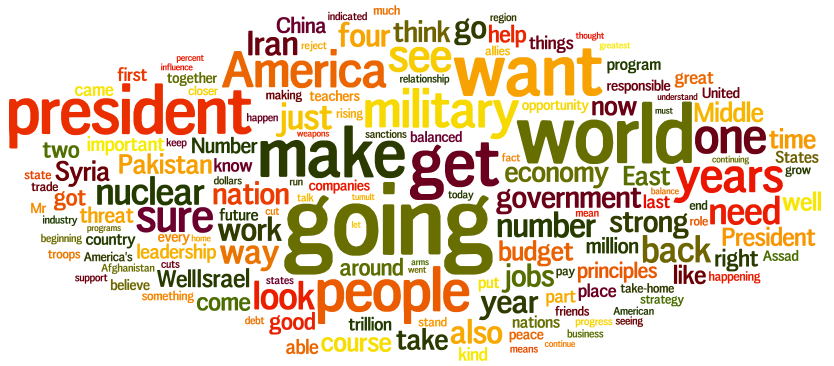
\includegraphics[scale=0.5]{img/wc_statiche/romney_wc.png}}
\caption[Due word cloud relative ai dibattiti tra i candidati alla presidenza statunitense.]{Due wordcloud relative ai dibattiti tra i candidati alla presidenza statunitense.}
\label{fig:obama_romney}
\end{figure}

In riferimento al web, si parla invece di \textbf{tag cloud}, con evidente richiamo ai tag, ovvero ai metadati che riassumono il contenuto di un sito internet. Ogni tag, rappresenta un link ad una specifica risorsa sul web, consentendo agli utenti di accedervi tramite l'utilizzo di keywords. Il loro utilizzo si � diffuso grazie al sito di \textit{photo sharing} Flickr\cite{flickr}, in cui i tag classificano in diverse categorie le foto che vengono condivise tra gli utenti.

Le parole di una word cloud sono tipicamente pesate in base all'importanza che esse ricoprono nel testo: pi� le parole hanno un font grande, pi� sono rilevanti. In questo modo, le word cloud permettono immediatamente di evidenziare ci� che � rilevante in un testo. Ci sono anche altri parametri da tenere in considerazione. In \cite{halvey}, Halvey et al. hanno valutato l'effetto di alcuni fattori: la posizione delle parole, la loro disposizione secondo l'ordine alfabetico e, come detto, la dimensione del font, si sono rivelati essere parametri importanti. Inoltre, hanno notato che gli utenti, piuttosto che leggere tutte le parole, danno uno sguardo generale alla word cloud. In un altro lavoro, Lohmann et al.\cite{Lohmann} hanno scoperto che parole posizionate vicino al centro catturano di pi� l'attenzione rispetto a parole vicine ai bordi, cos� come parole posizionate in alto a sinistra vengono percepite prima delle altre da parte degli utenti.

\subsection{Applicazioni}
Esistono diversi strumenti per la creazione di word cloud. Un tool web based molto popolare, Wordle\cite{Viegas:2009}, grazie alle qualit� grafiche e alle sue funzionalit�, ha permesso la diffusione delle word cloud come potente strumento per riassumere e analizzare un testo. Con Wordle, ad esempio, � possibile impostare alcuni parametri in modo da personalizzare la word cloud finale, come il numero delle parole, il colore, gli angoli di disegno ecc.. Tuttavia, Wordle non riesce a catturare le relazioni semantiche tra le parole, propriet� che pu� rivelarsi cruciale nell'analisi e nella comprensione di un testo. 
Per ovviare a ci�, � stato proposto un ulteriore strumento, basato su Wordle, chiamato ManiWordle\cite{kohk}, il quale offre un buon livello di interazione con l'utente, permettendo a quest'ultimo di manipolare il disegno finale e di modificare le parole visualizzate in termini di posizione, colore e orientamento, risultando quindi pi� flessibile di Wordle. Un altro sistema, SparkClouds\cite{lee}, tramite l'uso delle \textit{sparklines}, mette in risalto i cambiamenti tra pi� word cloud. Collins et al.\cite{collins}, hanno presentato Parallel Tag Clouds, uno strumento in grado di visualizzare le differenze tra i testi scritti di un ricco dataset. FacetAtlas\cite{facetatlas}, invece, � un'applicazione che, tramite grafici e mappe di densit�, visualizza le relazioni che intercorrono tra i documenti di una vasta collezione di testi.

In generale, dunque, negli anni, sono state sviluppate varie applicazioni che generano word cloud, ognuna con pregi e difetti, le quali permettono di comparare diversi documenti da pi� prospettive. Il nostro lavoro � in direzione di quello che � il trend degli ultimi tempi, cio� quello di creare word cloud semantiche, in cui la disposizione delle parole riflette la loro correlazione semantica.

\section{Word cloud semantiche}\label{wc_stat:sem}
Recentemente, la maggior parte dei tool che generano word cloud si � posta come obiettivo quello di raggruppare semanticamente le parole estratte, utilizzando tecniche di elaborazione del linguaggio naturale per correlare parole simili tra loro. Infatti, la possibilit� di disegnare, vicine nella word cloud, parole correlate semanticamente, pu� migliorare l'esperienza dell'utente, come notato da Deutsch et al. in \cite{Deutsch}.

Tree Cloud\cite{gambette}, ad esempio, � un applicazione in cui le parole vengono disposte secondo un albero, in modo tale da preservare la loro vicinanza semantica. In \cite{cui}, Cui et al., tramite misure di similarit�, mirano a collocare, vicine nel disegno, parole correlate semanticamente, utilizzando poi un metodo force directed per compattare la word cloud. Wu et al.\cite{seam}, utilizzano una tecnica ispirata al \textit{seam carving} per ottenere una word cloud semantica e compatta. Questo lavoro di tesi, invece, prende spunto dal recente lavoro svolto da Kobourov et al.\cite{kobourov}, in cui vengono implementati due nuovi algoritmi di visualizzazione, da confrontare con altri algoritmi esistenti, per analizzare la qualit� delle word cloud in base a diverse metriche, ovviamente partendo dalla base comune costituita dalla coerenza semantica nella disposizione delle parole. 
\onehalfspacing

%%CAPITOLO 3: =======================================

\chapter{Word cloud dinamiche}
Il concetto di word cloud dinamica, che � l'obiettivo di questa tesi, � descritto, dal punto di vista algoritmico, nel seguente capitolo. 
\\ \\
La sezione \ref{wc_din:def} offre una visione generale sul concetto di word cloud dinamica (cio� tempo variante), sullo stato dell'arte e alcuni cenni sui possibili contesti d'uso. Il paragrafo \ref{wc_din:algs} espone, fase per fase, il processo che consente di creare una word cloud statica da un testo di input, tenendo ben presente il vincolo di vicinanza semantica tra parole simili. Ogni fase � composta da diversi algoritmi, che vengono descritti progressivamente. Il capitolo quindi si chiude con la sezione \ref{wc_din:din_algs}, che presenta i passaggi necessari ad ottenere dinamicit� nel layout finale.

\section{Definizioni e applicazioni}\label{wc_din:def}
\subsection{Word cloud dinamiche e stato dell'arte}
Negli ultimi anni, sono state proposte diverse applicazioni per la creazione di word cloud. Oltre alla distinzione tra word cloud semantiche e non semantiche, � possibile suddividere tali applicazioni sulla base di due ulteriori categorie: word cloud \textbf{statiche} e word cloud \textbf{dinamiche} (o \textbf{tempo varianti}). La principale differenza tra queste due classi � chiaramente costituita dal fattore tempo: le word cloud dinamiche, infatti, hanno come obiettivo quello di illustrare l'evoluzione temporale di un documento o di un set di documenti. I grafici a barre, per esempio, sono tipicamente utilizzati per rappresentare l'andamento temporale di una qualche variabile e consentirne l'analisi visuale\cite{byron}\cite{havre}; Dubinko et al.\cite{dubinko} hanno sviluppato un tool che mostra l'evoluzione dei tag in Flickr e che permette l'interazione con gli utenti. Un lavoro rilevante, che tiene conto dell'evoluzione semantica e temporale di un insieme di documenti � stato effettuato da Cui et al.\cite{cui}: essi hanno proposto un sistema che abbina un grafico di tendenza (\textit{trend chart}) alle word cloud ottenute da documenti appartenenti ad una collezione. 

Sebbene tutti questi lavori abbiano come finalit� quella di visualizzare l'andamento temporale di un insieme di testi scritti, le informazioni spaziali e temporali sono rappresentate da immagini statiche. Diversamente, un lavoro interessante � stato svolto di recente da Chi et al.\cite{chi}, in cui viene mostrato il progresso temporale di un set di documenti tramite l'utilizzo di tecniche di \textit{morphing}\footnote{Il morphing consiste nella trasformazione fluida, graduale e senza soluzione di continuit� tra due immagini di forma diversa\cite{wiki:morphing}.}, che permettono di passare gradualmente da una word cloud di un documento ad un'altra di un altro documento, modificandone anche la forma (figura \ref{fig:morph_chi}). Tuttavia, come in\cite{cui}, la visualizzazione � relativa ad un insieme di documenti, quindi il periodo temporale preso in considerazione � piuttosto ampio. Inoltre, in questo studio, non viene affrontato l'aspetto semantico nei layout di ogni word cloud.  
\begin{figure}
\centering
{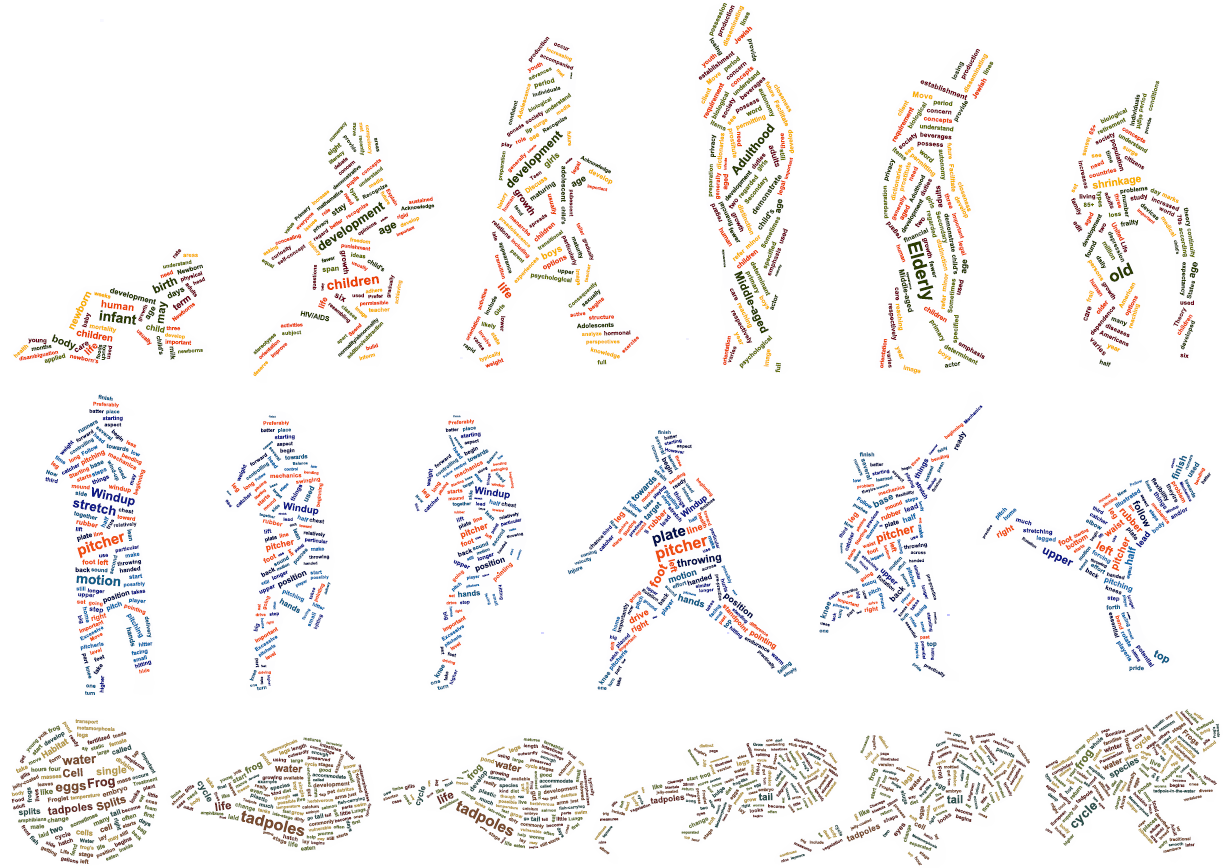
\includegraphics[scale=0.55]{img/wc_dinamiche/morphing_wc.png}}
\caption[Evoluzione di diverse word word cloud tramite tecniche di morphing.]{Evoluzione di diverse word word cloud tramite tecniche di morphing\cite{chi}: in alto, � mostrato il ciclo di vita dell'uomo; in mezzo, sono illustrati i movimenti effettuati dal pitcher nel baseball; in basso, infine, � mostrato il ciclo di vita di una rana.}
\label{fig:morph_chi}
\end{figure}

Il nostro lavoro, invece, a differenza degli altri citati precedentemente, si pone come finalit� quello di mostrare l'evoluzione di un solo testo, cio� il periodo temporale da cui si genera la word cloud � (relativamente) breve, poich� si prende in considerazione un solo documento. Per questo motivo, diventa significativo avere delle animazioni, che permettono di visualizzare l'evoluzione della word cloud insieme all'avanzamento dell'input. A tal fine, viene utilizzata una tecnica di morphing tra le word cloud generate in diversi istanti di tempo durante l'elaborazione del testo, rispettando, se possibile, il vincolo di vicinanza geometrica tra parole correlate semanticamente. Inoltre, � anche importante che non ci siano troppe differenze tra word cloud estratte in istanti successivi, ovvero parole che si muovono eccessivamente: l'utente potrebbe disorientarsi e perdersi durante l'evoluzione del testo, per cui la sua mappa mentale non deve cambiare in modo radicale. Da notare che, rispettare il vincolo di vicinanza semantica, insieme alla coerenza della mappa mentale, pu� costituire un compito impegnativo, dal momento che questi due vincoli costituiscono obiettivi contrastanti fra loro.
\subsection{Applicazioni}
I possibili utilizzi delle word cloud dinamiche, prodotte a partire da un unico testo di input, riguardano i contesti in cui si vuole visualizzare l'evoluzione di un generico documento relativo ad un breve periodo di tempo. Gli ambiti applicativi sono diversi, tra cui quello: 
\begin{itemize}
\item didattico, allo scopo, per esempio, di fornire uno strumento di ausilio nella comprensione di un testo;
\item divulgativo, per mostrare l'evoluzione di un discorso. Ci� pu� essere di grande utilit� per persone non udenti oppure nel caso di video riprodotti in luoghi con scarsa udibilit�; 
\item statistico, per illustrare l'evoluzione, in un breve periodo di tempo (ad esempio, in una giornata), dei trending topic dei vari social network;
\item ecc...
\end{itemize}

\section{Algoritmi di generazione di una word cloud semantica}\label{wc_din:algs}
Tutti gli algoritmi di visualizzazione di una word cloud ricevono in input un grafo pesato, i cui vertici sono le parole, rappresentate da rettangoli. Tuttavia, sono necessari alcuni passi di preprocessing, che consentono di estrarre questa informazione dall'input. L'algoritmo di visualizzazione disegna, per quanto possibile, le parole pi� simili vicine tra loro. Il processo di creazione di una word cloud � indicato in figura \ref{fig:pipeline}. Infine, viene applicato un algoritmo di clustering per assegnare lo stesso colore a parole dello stesso cluster.
\begin{figure}
\centering
{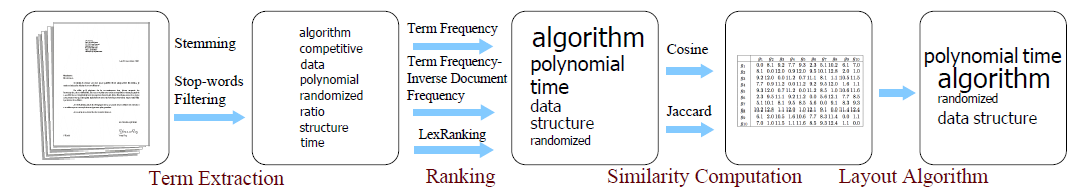
\includegraphics[scale=0.6]{img/wc_dinamiche/creation_steps.png}}
\caption[Generazione di una word cloud semantica.]{Generazione di una word cloud semantica.}
\label{fig:pipeline}
\end{figure}
\\ \\
Di seguito vengono prima esposti alcuni concetti teorici utilizzati nella definizione degli algoritmi. Successivamente, vengono descritte le varie fasi necessarie alla realizzazione di una word cloud semantica. 
\subsection{Riferimenti teorici}
\subsubsection{Grafo}
Un \textbf{grafo} $G$ � una coppia $(V,E)$, dove $V$ � un insieme finito ed $E$ � una relazione binaria in $V$. L'insieme $V$ � chiamato insieme dei vertici di $G$, mentre l'insieme $E$ � detto insieme degli archi di $G$. Un grafo si dice \textbf{orientato} se l'insieme degli archi $E$ � formato da coppie di vertici ordinate, altrimenti il grafo si dice \textbf{non orientato}. Dati due vertici $u,v \in V$, un arco che collega i due vertici � denotato con $(u,v)$ ed � detto \textbf{incidente} nei vertici $u$ e $v$. In tal caso, $u$ e $v$ sono gli \textbf{estremi} di $(u,v)$, e $u$ e $v$ sono \textbf{adiacenti}. Se un arco entra ed esce nello stesso vertice, allora si dice \textbf{cappio} (\textbf{self-loop}).

Dato un grafo $G=(V,E)$, si dice che $G'=(V'E')$ � un \textbf{sottografo} di $G$ se $V' \subseteq V$ ed $E' \subseteq E$. Dato un insieme $V' \subseteq V$, il sottografo di $G$ \textbf{indotto} da $V'$  � il grafo $G'=(V',E')$, dove $E' = \{(u,v) \in E : u,v \in V' \}$.
\subsubsection{Cammini e cicli}
Un \textbf{cammino} di lunghezza $k$ da un $u$ a $v$, con $u,v \in V$, in un grafo non orientato $G=(V,E)$, � una sequenza di vertici $(v_{0},v_{1},...,v_{k})$ tali che $u = v_{0}, v=v_{k}$ e $(v_{i-1},v_{i}) \in E$, con $0 \leq i \leq k$. La lunghezza del cammino � pari al numero di archi in $E$. \\
Un \textbf{ciclo} � un cammino $(v_{0},v_{1},...,v_{k})$ in cui $v_{0}=v_{k}$. Un cammino � \textbf{semplice} se tutti i suoi vertici sono distinti. Un ciclo � \textbf{semplice} se i vertici $(v_{0},v_{1},...,v_{k-1})$ sono distinti. Un cappio � un ciclo di lunghezza unitaria.

\subsubsection{Altre propriet� dei grafi}
Un grafo non orientato $G=(V,E)$ � \textbf{connesso} se ogni coppia di vertici � collegata attraverso un cammino, ovvero se ogni vertice � raggiungibile da ogni altro vertice. Le \textbf{componenti connesse} di un grafo $G$ sono i sottografi massimali connessi di $G$.

Un grafo non orientato � detto \textbf{aciclico} se non contiene cicli.  Un grafo non orientato e aciclico � una \textbf{foresta}; un grafo connesso, non orientato e aciclico � un \textbf{albero}. Si noti che ciascuna componente connessa di una foresta � un albero.

Un grafo non orientato si dice \textbf{bipartito} se l'insieme dei vertici $V$ pu� essere partizionato in due insiemi $U$ e $V$ tali che, se $(u,v) \in E$, allora $u \in U$ e $v \in V$ oppure $u \in V$ e $v \in U$. Un \textbf{matching} di $G$ � un insieme di archi tali che non ci sono due archi nell'insieme con un vertice in comune.
\subsection{Estrazione keywords}\label{wc_din:word_ext}
Il processo di estrazione delle keywords prevede una serie di passaggi preliminari, derivati da tecniche di elaborazione del linguaggio naturale, le quali predispongono, in maniera appropriata, il testo in ingresso all'algoritmo di estrazione delle parole.

Innanzitutto, il testo viene suddiviso in frasi. Poi, ogni sequenza di caratteri viene scomposta in \textit{token} (insiemi di caratteri, ad esempio parole, punteggiatura, numeri, simboli ecc...): ci� pu� essere eseguito mediante l'ausilio di librerie di elaborazione del linguaggio naturale (e.g. \textit{Apache OpenNLP}\cite{opennlp}). Successivamente, dal testo vengono eliminate le \textit{stop words}, cio� articoli, congiunzioni, parole di uso comune che sono poco rilevanti dal punto di vista informativo. Le parole rimanenti vengono quindi raggruppate in base alle rispettive radici (in inglese, \textit{stem}), tramite un algoritmo di \textit{stemming}: in questo modo, ad esempio, parole come \textit{play}, \textit{player}, \textit{played} e \textit{playing} vengono raggruppate secondo la radice comune \textit{play}. Nella nostra implementazione, � stato utilizzato il noto algoritmo \textbf{Porter Stemmer}\cite{porter}. Alla fine, nella word cloud finale, viene visualizzata la variante pi� frequente della parola.

Una volta eseguiti questi passaggi, si procede all'estrazione delle parole e al loro ranking in modo da trovare quelle pi� rilevanti, utilizzando tecniche di Information Retrieval. Ogni algoritmo assegna alle parole un punteggio e ne seleziona le $n$ pi� frequenti, dove $n$ � il numero di parole da visualizzare nella word cloud.
\\ \\
In questo lavoro di tesi sono state utilizzate diverse tecniche di estrazione delle keywords, qui di seguito esposte.
\subsubsection{Term Frequency (TF)}
Il modo pi� intuitivo di assegnare un peso alle parole consiste nel contare le loro singole occorrenze. Questo � ci� che viene fatto dall'algoritmo Term Frequency. Tuttavia, la rilevanza di un termine non aumenta linearmente con il numero delle occorrenze, in quanto documenti di una certa lunghezza potrebbero contribuire di pi� rispetto a documenti pi� corti, cio� potrebbero avere un peso maggiore nel conteggio delle occorrenze. Il calcolo della frequenza potrebbe quindi essere influenzato da questo fattore, per cui il punteggio di ogni parola spesso viene scalato tramite una qualche funzione. In tabella \ref{tab:tf}, sono riportate le tipiche funzioni che vengono utilizzate per pesare tale contributo (come indicato in \cite{manning}), dove l'argomento $ \textit{tf}_{t,d} $ indica la frequenza del termine $t$ nel documento $d$. 

\begin{table}[!htbp]
\centering
\renewcommand\arraystretch{1.4}
\begin{tabular}{|c|c|}
\hline
\textbf{Tipo funzione} &  \textbf{Peso} \\
\hline
Binaria & $0$,$1$ \\
\hline
Lineare & $ \textit{tf}_{t,d} $ \\
\hline
Radice quadrata & $ \sqrt{\textit{tf}_{t,d}} $ \\
\hline
Logaritmo & $ 1 + \log{\textit{tf}_{t,d}} $ \\
\hline
Doppia normalizzazione con parametro $K$ & $K + (1-K)* \frac{\textit{tf}_{t,d}}
{\max_{t' \in d} \textit{tf}_{t',d}}$ \\
\hline
\end{tabular}
\caption{Term Frequency ranking: funzioni}
\label{tab:tf}
\end{table}
Ad ogni modo, pur dopo aver rimosso le stop words, l'algoritmo Term Frequency tende ad assegnare punteggi troppo alti a termini poco rilevanti. Termini rari, invece, hanno contenuto informativo pi� alto rispetto a termini frequenti, per cui ad essi devono essere assegnati punteggi pi� elevati. In particolare, si definisce il parametro \textbf{IDF} (\textbf{Inverse Document Frequency}) di un termine $t$ la quantit�:
\begin{equation}
\textit{idf}_{t} = \log{\frac{N}{\textit{df}_{t}}},
\end{equation} 
dove $N$ � la dimensione di una collezione di documenti, mentre la quantit� $\textit{df}_{t}$ � detta \textit{document frequency}, che rappresenta il numero totale di documenti in cui il termine $t$ compare. Per termini frequenti in una collezione, tale valore tende a zero, mentre per termini meno frequenti il punteggio sar� pi� alto. Lo scaling che viene applicato � solitamente logaritmico, con qualche variante.

\subsubsection{TF-IDF}
Ora si possono combinare le due definizioni di TF e IDF per produrre un ulteriore algoritmo, noto come TF-IDF, il quale assegna, ad ogni termine $t$ di un documento $d$, la quantit�
\begin{equation}
\textit{tf-idf}_{t,d} = \textit{tf}_{t,d} \times \textit{idf}_{t}.
\end{equation}
Ne segue che:
\begin{itemize}
\item se $t$ � un termine comune nella collezione, avr� un $\textit{tf}_{t,d}$ alto, ma un $\textit{idf}_{t}$ vicino a zero, per cui $\textit{tf-idf}_{t,d}$ sar� tendente a zero;
\item se $t$ � un termine raro nella collezione, ma frequente nel documento $d$, allora avr� entrambi i contributi elevati, da cui ne deriva che $\textit{tf-idf}_{t,d}$ sar� alto.
\end{itemize} 
In pratica, con questo approccio, vengono filtrati i termini molto comuni, mentre quelli davvero rilevanti per il documento vengono estratti.

Uno degli schemi pi� noti in letteratura per calcolare la $\textit{tf-idf}_{t}$, come suggerito in \cite{manning} ed adottato in questa tesi, � il seguente:
\begin{equation}
\textit{tf-idf}_{t,d} = (1 + \log{\textit{tf}_{t,d}}) \times \log{\frac{N}{\textit{df}_{t}}}.
\end{equation}
\subsubsection{LexRank}
Il terzo algoritmo di ranking � LexRank\cite{lexrank}, gi� usato in \cite{seam} per la creazione di word cloud semantiche.  Tale algoritmo prende spunto da PageRank\cite{pagerank}, algoritmo utilizzato da Google per assegnare un punteggio alle pagine web e quindi migliorare le ricerche che si effettuano con il noto motore di ricerca.

LexRank � un algoritmo basato su un grafo $ G=(V,E) $, dove i vertici sono le parole, collegati da archi che rappresentano le co-occorrenze di due parole all'interno di una frase. Ogni arco $(i,j)$ ha infatti un peso $w_{ij}$, pari al numero di occorrenze della parola $i$ e della parola $j$ all'interno di una stessa frase. I punteggi vengono poi calcolati sfruttando il concetto di centralit� dell'autovettore definito da $G$. Tale valore di centralit� viene distribuito, da ogni vertice, ai suoi vicini. \\ Sia quindi $R$ il vettore di ranking, di dimensione $1 \times \vert V \vert$, dove $\vert V \vert$ � il numero dei nodi di $G$. Possiamo definire (per approfondimenti, consultare \cite{lexrank})
\begin{equation}
R = dM \cdot R + (1-d)p
\end{equation}
\begin{equation}
P \cdot R = \lambda R
\end{equation}
\begin{equation}
P = dM + (1-d)p \cdot 1^T
\end{equation}
dove:
\begin{itemize}
\item $d$ � il \textit{damping factor}, tipicamente scelto nell'intervallo $[0.1,0.2]$, come suggerito in \cite{lexrank};
\item $M$ � la matrice delle co-occorrenze normalizzata, avente dimensioni $\vert V \vert \times \vert V \vert$ e tale che la somma di ogni colonna sia pari a 1;
\item $p$ � il vettore delle probabilit�, di dimensione $1 \times \vert V \vert$, con ogni elemento pari a $1/\vert V \vert$;
\item $R$ � l'autovettore corrispondente al pi� grande autovalore di $M$ e pu� essere ricavato tramite l'algoritmo \textit{Power Method}, usato in \cite{lexrank}.
\end{itemize}
Alla fine, le parole estratte saranno costituite dai primi $n$ valori di $R$.

\subsection{Calcolo similarit�}\label{par:simil}
Il passo successivo � quello di calcolare la similarit� tra le keywords, ovvero quanto esse sono correlate tra loro. Data la lista delle $n$ parole estratte, viene calcolata la matrice $n \times n$ delle similarit� tra coppie di parole. Ogni valore � compreso tra 0 (nessuna correlazione) e 1 (massima correlazione). Esistono diversi algoritmi per il calcolo delle similarit�. Tutti usano uno spazio vettoriale di dimensione $n$ (pari al numero di parole estratte), dove il generico vettore $w_{i} = \{w_{i1},w_{i2},...,w_{in}\}$ rappresenta la co-occorrenza della $i$-esima parola con le altre $n-1$ parole. 
\\ \\ 
Di seguito sono esposte le tecniche di calcolo da noi implementate.

\subsubsection{Cosine Similarity}
La cosine similarity tra due vettori $w_{i}$ e $w_{j}$ viene calcolata come:
\begin{equation}
sim_{ij} = \frac{w_{i} \cdot w_{j}}{\vert\vert w_{i} \vert\vert \, \vert\vert w_{j} \vert\vert}
\end{equation}
In pratica, tale quantit� corrisponde alla misura dell'angolo formato tra i vettori $w_{i}$ e $w_{j}$. Se la similarit� � 1, allora l'angolo formato � pari $0�$, mentre se la similarit� � 0, allora i due vettori sono perpendicolari (angolo di intersezione $90�$) e non condividono alcuna frase.

\subsubsection{Jaccard Similarity}
La Jaccard similarity � definita come il rapporto tra il numero delle frasi condivise tra due parole e il numero totale delle frasi in cui esse compaiono. In formule:
\begin{equation}
sim_{ij} = \frac{\vert S_{i} \cap S_{j} \vert}{\vert S_{i} \cup S_{j} \vert},
\end{equation}
dove $S_{i}$ e $S_{j}$ sono, rispettivamente, l'insieme delle frasi in cui compare la parola $i$ e l'insieme delle frasi in cui compare la parola $j$.

\subsubsection{Jaccard Similarity estesa}
Un ulteriore modo per il calcolo della similarit� � rappresentato dalla Jaccard similarity estesa (anche nota come \textbf{coefficiente di Tanimoto}), definita come:
\begin{equation}
sim_{ij} = \frac{w_{i} \cdot w_{j}}{\vert\vert w_{i} \vert\vert^2 + \vert\vert w_{j} \vert\vert^2 - w_{i} \cdot w_{j}}
\end{equation}
Tale misura si riduce alla Jaccard Similarity nel caso di vettori binari.

\subsection{Creazione word cloud}
Gli algoritmi che producono word cloud ricevono in input una collezione di $n$ rettangoli (detti \textit{bounding box}), corrispondenti alle $n$ parole estratte, ognuno dei quali avente dimensioni proporzionali alla rilevanza della parola, e la matrice delle similarit� (di dimensione $n \times n$), dove ogni elemento � in $[0,1]$. L'output � costituito da un insieme di rettangoli sul piano e non sovrapposti. All'interno dei rettangoli sono disegnate le parole. Ovviamente, nel layout finale, saranno visibili solo le parole.
\\ \\
In questo lavoro di tesi sono stati utilizzati tre algoritmi: Context-Preserving Word Cloud Visualization\cite{cui}, Star Forest\cite{kobourov} e Cycle Cover\cite{kobourov}. Tutti e tre gli algoritmi sono stati pensati per una visualizzazione statica della word cloud, per cui essi sono stati modificati per tener conto dell'aspetto dinamico (pi� tardi vedremo come).

\subsubsection{Context-Preserving Word Cloud Visualization (CPWCV)}
Questo algoritmo, introdotto da Cui et al. in\cite{cui}, mira a soddisfare il vincolo di vicinanza geometrica tra parole correlate semanticamente in due passi: prima di tutto, viene calcolata, a partire dal contributo di ogni elemento $sim_{i,j}$ della matrice di similarit�, la distanza tra coppie di parole, pari a $d_{i,j}=1-sim_{i,j}$. Tale valore corrisponde alla distanza ideale tra la generica coppia di parole $(i,j)$ in uno spazio $n$-dimensionale. Viene quindi applicato uno \textit{scaling multidimensionale} (MDS), in modo da ottenere, su uno spazio bidimensionale, una prima collocazione delle parole tale da rispettare, approssimativamente, le distanze calcolate. Per preservare il posizionamento relativo tra le parole, si utilizza la \textit{triangolazione di Delaunay}\cite{delaunay}. Ci� crea un layout iniziale con occupazione dello spazio non ottimale. Perci� si applica un algoritmo force directed, che aggiorna le posizione delle parole mantenendo invariata la topologia del grafo, ovvero le relazioni semantiche tra le parole. Tale algoritmo si basa su tre principi:
\begin{itemize}
\item Principio di compattazione: questo principio mira a rimuovere, per quanto possibile, gli spazi tra le parole, in modo da ottenere un layout compatto;
\item Principio di non sovrapposizione: questa condizione richiede che le parole non siano sovrapposte, propriet� fondamentale per la leggibilit� della word cloud;
\item Principio di planarit�: per mantenere le relazioni semantiche tra le parole, il grafo � bene che sia planare, anche se ci� non � strettamente necessario. Inoltre imporre questa condizione pu� portare ad uno spreco di spazio.
\end{itemize}
Seguendo tali principi, la word cloud che si ottiene � compatta, facilmente leggibile e semanticamente coerente. Ognuna di queste propriet� � ottenibile applicando, rispettivamente, una forza elastica, una forza repulsiva e una forza attrattiva.

\subsubsection{Star Forest}
Introdotto in\cite{kobourov} da Kobourov et. al, Star Forest consiste in una \textbf{foresta di stelle}. Una foresta di stelle � una foresta dove le componenti connesse sono costituite da stelle. Una \textbf{stella} � un albero di profondit� massima pari a 1. 
\\ \\
L'algoritmo � composto da una sequenza di tre passaggi fondamentali:
\begin{enumerate}
\item Partizionamento del grafo, in modo da ottenere una foresta di stelle.
\item Applicazione dello scaling multidimensionale alla matrice delle distanze, ottenuta da quella delle similarit� tra coppie di parole, con conseguente creazione della word cloud per ogni stella.
\item Compattazione delle singole word cloud realizzate, da cui ne deriva il risultato finale.
\end{enumerate}
Le stelle vengono estratte dal grafo in modo \textit{greedy}. Si cerca un vertice $v$ i cui vertici adiacenti abbiano peso massimo, cio� tali che la somma $ \sum\nolimits_{u \in V} sim(u,v) $ sia massima. Si assume dunque che il vertice $v$ sia il centro della stella, mentre l'insieme dei vertici $V - \{v\}$ forma l'insieme delle foglie. Vengono scelte le parole adiacenti a $v$ e tali parole vengono rimosse dal grafo. Si ripete la procedura con grafi via via pi� piccoli, finch� non ci saranno pi� vertici.

\begin{figure}
\centering
{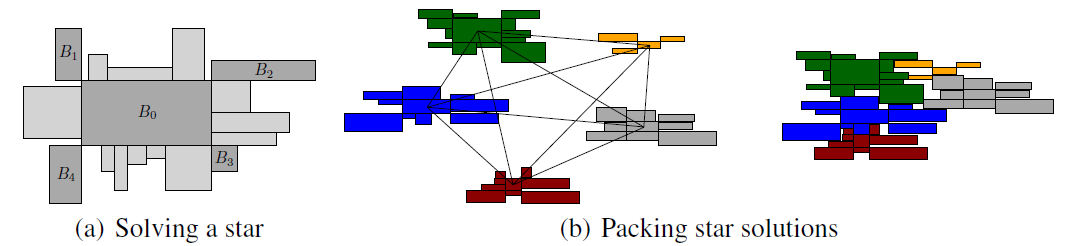
\includegraphics[scale=0.6]{img/wc_dinamiche/starforest.png}}
\caption[Algoritmo Star Forest.]{Algoritmo Star Forest.}
\label{fig:starforest}
\end{figure}

Selezionare il miglior insieme di parole adiacenti al centro $v$ della stella � un problema equivalente al noto problema dello zaino (\textit{Knapsack Problem}): dati $N$ oggetti, ognuno avente un peso e un valore, si vuole scegliere l'insieme di oggetti di maggior valore da inserire in uno zaino avente peso massimo sopportato pari a $W$. Sia dunque $B_{0}$ il bounding box corrispondente al centro della stella. In ogni soluzione ottima, ci sono quattro bounding box $B_{1},B_{2},B_{3},B_{4}$, ognuno avente un lato che contiene uno degli angoli di $B_{0}$ (figura \ref{fig:starforest}(a)). Dati $B_{1},B_{2},B_{3},B_{4}$, il problema si riduce ad assegnare ad ogni box $B_{i}$ uno dei quattro lati di $B_{0}$. Questo problema � equivalente ad un'istanza del problema dello zaino: il peso del bounding box $B_{i}$ � proporzionale alle sue dimensioni, dove la sua base � moltiplicata per la base di $B_{0}$ e l'altezza � moltiplicata per l'altezza di $B_{0}$, mentre il valore � pari al peso dell'arco che collega $B_{0}$ a $B_{i}$. L'algoritmo viene eseguito, in senso orario, a partire dal lato superiore di $B_{0}$. Per risolvere le istanze del problema, si utilizza l'algoritmo di approssimazione in tempo polinomiale descritto in\cite{ibarra}.

Le soluzione ottenute per le singole stelle vengono dunque messe insieme in un layout compatto, senza sovrapposizioni tra le parole e nel quale le relazioni semantiche tra le parole sono preservate (figura \ref{fig:starforest}(b)). Per ogni coppia di stelle $s_{1},s_{2}$, si ottiene la similarit� media tra le parole di $s_{1}$ e $s_{2}$ come $ sim(s_{1},s_{2}) = 
\dfrac{\sum\nolimits_{u \in s_{1}} \sum\nolimits_{v \in s_{2}} sim(u,v)}{\vert s_{1} \vert \vert s_{2} \vert}$. Si utilizza dunque l'MDS, con la distanza ideale tra le coppie di stelle posta uguale a
$ k(1 - sim(s_{1},s_{2})) $, dove $k$ � un fattore di scala, ottenendo cos� un primo layout. Poi, per compattare il disegno, si applica un algoritmo force directed. Da notare che esso viene applicato sulle stelle, non sulle singole parole. Tale algoritmo fa uso di due forze: 
\begin{itemize}
\item attrattiva, per rimuovere gli spazi vuoti, uguale a 
$ k_{a}(1 -  sim(s_{1},s_{2}))\Delta l$, con $\Delta l$ pari alla minima distanza tra i centri delle due stelle;
\item repulsiva, per evitare sovrapposizioni tra le varie parole, pari a  
$ k_{r}min(\Delta x,\Delta y)$, dove $\Delta x$ ($\Delta y$) corrisponde alla larghezza (altezza) della regione di spazio in sovrapposizione.
\end{itemize} 
Come ogni algoritmo force directed, questo metodo aggiorna le posizioni delle stelle iterativamente.

\subsubsection{Cycle Cover}
Questo algoritmo � stato proposto, come Star Forest, da Kobourov et. al in\cite{kobourov}. Esso si basa sull'estrazione di un sottografo planare dal grafo $G=(V,E)$ definito dalla matrice di similarit�. Tale sottografo � composto da un insieme disgiunto di cicli di peso massimo ed � denominato, appunto, \textit{cycle cover}.

L'algoritmo che calcola il cycle cover estrae, dal grafo $G$, un grafo bipartito $H$. Si inizializza infatti $H$ con i vertici di $G$. Poi, per ogni $v \in V(G)$, si aggiunge un vertice $v' \in V(H)$, e per ogni arco $(u,v) \in E(G)$, vengono creati due archi, $(u',v)$ e $(u,v') \in E(H)$, aventi peso pari a $sim(u,v)$. Il grafo $H$ risultante � bipartito per costruzione ed � facile ricavare un matching di peso massimo. Tale matching consiste in un insieme di cammini e cicli disgiunti di $G$, in quanto ogni $u$ � accoppiato a $v'$ e ogni $u'$ � accoppiato a $v$.

\begin{figure}
\centering
{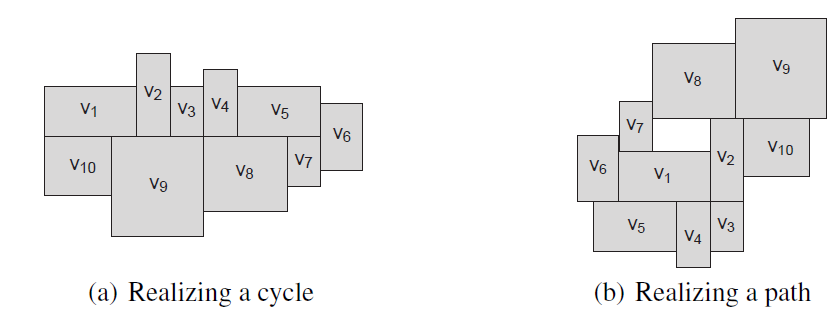
\includegraphics[scale=0.7]{img/wc_dinamiche/cyclecover.png}}
\caption[Algoritmo Cycle Cover.]{Algoritmo Cycle Cover.}
\label{fig:cyclecover}
\end{figure}

Fissato dunque un ciclo $(v_{1},v_{2},...,v_{n})$, sia $t$ il massimo indice  tale che $ \sum\nolimits_{i \leq t} w_{i} \leq \sum\nolimits_{i \leq n} w_{i}/2 $, dove $w_{i}$ � la base del bounding box corrispondente alla parola i-esima. I vertici $v_{1},v_{2},...,v_{t}$ vengono collocati orizzontalmente da sinistra verso destra, mentre i vertici $v_{n},v_{n-1},...,v_{t+2}$ vengono collocati da destra verso sinistra. In entrambi i casi, i vertici sono allineati su una stessa linea (figura \ref{fig:cyclecover}(a)). Rimane da piazzare il vertice $v_{t+1}$, in contatto tra $v_{t}$ e $v_{t+2}$. Si sceglie il gruppo di vertici (superiore o inferiore) i cui rettangoli hanno la minima larghezza oppure lo si pone a met� tra  $v_{t}$ e $v_{t+2}$. I cicli vengono convertiti in cammini se sono composti da pi� di 10 vertici. In tal caso, dopo aver posizionato i vertici $v_{1}$ e $v_{2}$ vicini l'un l'altro, si procede a piazzare il generico vertice $v_{i}$ in modo tale che tocchi $v_{i-1}$ nel primo spazio disponibile in senso orario, ottenendo cos� un layout a spirale.

Successivamente, cos� come nell'algoritmo Star Forest, le soluzioni individuali realizzate vengono messe insieme. Poi si applica lo stesso algoritmo force directed, descritto precedentemente, per compattare il disegno e rimuovere eventuali intersezioni tra le parole.

\subsection{Clustering}
Una volta ottenuto il layout, si prosegue con l'applicazione di un algoritmo di \textit{clustering}, il quale suddivide le parole in pi� gruppi (\textit{cluster}). Ad ogni cluster viene assegnato un colore diverso e ogni colore identifica un diverso raggruppamento semantico. In generale, l'obiettivo del clustering � quello di ottenere che gli oggetti di ogni cluster siano il pi� possibile simili tra loro, o comunque che la loro correlazione sia pi� alta rispetto a quella con oggetti di cluster diversi.
\\ \\
L'algoritmo di clustering utilizzato in questa tesi � K-means++, proposto da Arthur et. al in\cite{arthur}, ed � una versione migliorata di uno dei pi� noti algoritmi in letteratura, K-means. Prima verr� quindi presentato K-means, per poi passare alla variante K-means++.

\subsubsection{K-means}
K-means � un tipo di algoritmo \textbf{prototype-based}, cio� basato sul concetto di \textbf{prototipo}, che � l'elemento pi� rappresentativo di un cluster. Infatti, un cluster � una collezione di oggetti in cui ogni oggetto � pi� simile al prototipo del rispettivo cluster piuttosto che ai prototipi di altri cluster. K-means definisce il prototipo in termini di \textbf{centroide}, tipicamente inteso come elemento medio di un insieme di punti.

La tecnica di clustering definita dal K-means � piuttosto semplice e intuitiva, oltre ad essere veloce, sebbene non ci sono garanzie riguardo l'accuratezza del risultato. In generale, dato un intero $K>0$ e un insieme di $n$ oggetti di un dataset $\chi$, si vogliono scegliere $K$ centroidi, tali da minimizzare (o massimizzare) la funzione obiettivo 
\begin{equation}\label{kmeans_formula}
\phi = \sum\limits_{i=1}^K \sum\nolimits_{x \in C_{i}} dist(x,c_{i}),
\end{equation}
dove $C_{i}$ � l'i-esimo cluster e $dist(x,c_{i})$ � una qualche misura di prossimit� tra il generico elemento $x \in C_{i} $ e il centroide $c_{i}$ dell'i-esimo cluster. In pratica, ci� che si vuole ottenere, sono $k$ cluster in cui gli oggetti appartenenti ad ogni cluster siano il pi� possibile simili tra loro. 
\\ \\
L'ottimizzazione della funzione obiettivo � un problema NP-completo, per cui l'approccio comunemente adottato prevede le seguenti fasi, che fanno convergere l'algoritmo ad una soluzione locale (figura \ref{fig:kmeans_ex}): 
\begin{enumerate}
\item Si scelgono $K$ centroidi $C=\{c_{1},...,c_{k}\}$.
\item Ogni elemento $x \in \chi$ viene associato al centroide pi� vicino. Ogni collezione di elementi associata a $c_{i}, i \in \{1,...,k\}$, forma un cluster.
\item Si aggiorna il centroide di ogni cluster.
\item I passi 2 e 3 vengono eseguiti iterativamente finch� non si osservano ulteriori variazioni nell'insieme dei centroidi.
\end{enumerate}
\begin{figure}
\centering
{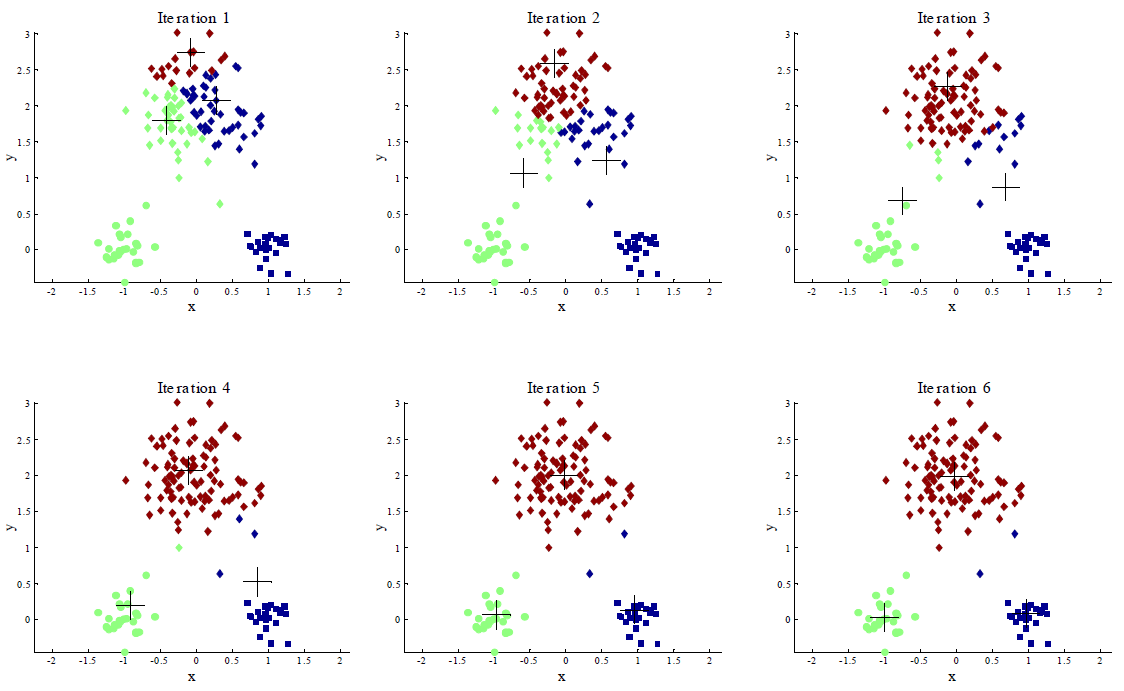
\includegraphics[scale=0.6]{img/wc_dinamiche/kmeans_ex.png}}
\caption[K-means: esempio di esecuzione dell'algoritmo. In questo caso si ottengono $K=3$ cluster.]{K-means: esempio di esecuzione dell'algoritmo\cite{tan}. In questo caso si ottengono $K=3$ cluster.}
\label{fig:kmeans_ex}
\end{figure}
Spesso i centroidi iniziali vengono selezionati in modo randomico, ma � possibile seguire diversi approcci. In ogni caso, supponendo di voler minimizzare la funzione obiettivo, l'idea dell'algoritmo � quella di decrementare, ad ogni esecuzione, il valore della funzione $\phi$, mediante i passi 2 e 3, finch� non vengono osservate variazioni nei centroidi. Infatti, $\phi$ � una funzione monotona decrescente, per cui ad ogni esecuzione il suo valore al massimo rimane invariato. Dal momento che ci sono $k^n$ raggruppamenti possibili, l'esecuzione dell'algoritmo termina sempre.

L'obiettivo dell'algoritmo, come detto, � quello di minimizzare (massimizzare) la funzione obiettivo $\phi$. Tale funzione, misura la qualit� del clustering tramite il calcolo della prossimit� (similarit�) tra il centroide $c_{i}$ e gli elementi del cluster $C_{i}$. Solitamente, i punti fanno parte di uno spazio $n$-dimensionale e come misura di prossimit� si utilizza la distanza euclidea. Ad ogni modo, ci sono diverse possibilit� per la scelta della misura di prossimit�, come indicato in tabella \ref{tab:prox_kmeans}\cite{tan}. 
\begin{table}[!htbp]
\centering
\renewcommand\arraystretch{1.4}
\begin{tabular}{|c|c|p{5cm}|}
\hline
\textbf{Funzione di prossimit�} &  \textbf{Centroide} & \textbf{Funzione obiettivo} \\
\hline
Manhattan & mediana & Minimizzare la somma delle distanze di ogni oggetto dal centroide del suo cluster \\
\hline
Euclidea & media & Minimizzare la somma delle distanze (al quadrato) di ogni oggetto dal centroide del suo cluster \\
\hline
Similarit� (coseno, Jaccard...) & media & Massimizzare (minimizzare) la similarit� (dissimilarit�) di ogni oggetto con il centroide del cluster di appartenenza  \\
\hline
Divergenza di Bregman & media & Minimizzare la somma della divergenza di Bregman di ogni oggetto con il centroide del cluster di appartenenza \\
\hline
\end{tabular}
\caption{K-means: scelte comuni per le misure di prossimit�.}
\label{tab:prox_kmeans}
\end{table}
\vspace{0.5cm}
\subsubsection{K-means\texorpdfstring{++}{}}
La differenza principale tra il K-means++ e il K-means classico consiste nell'inizializzazione dell'algoritmo, ovvero nella scelta dei $K$ centroidi iniziali, da cui dipende la qualit� del clustering finale. La fase di inizializzazione, infatti, consiste di diversi passaggi, di seguito esposti: 
\begin{enumerate}
\item Si sceglie il primo centroide $c_{1}$ in modo casuale tra tutti i punti (nel nostro caso le parole).
\item Per ogni altro elemento del dataset, $x \in \chi$, si calcola la distanza $dist(x,c_{i})$ tra $x$ e il centroide pi� vicino $c_{i}$ tra quelli gi� selezionati.
\item Un elemento generico $x$ pu� quindi diventare un centroide con probabilit� pari a $\dfrac{dist(x,c_{i})^2}{\sum\nolimits_{x \in \chi} dist(x,c_{i})^2} $.
\item Si ripetono gli step 2 e 3 finch� non si hanno $K$ centroidi.
\item Avendo ottenuto un insieme di $K$ centroidi, si pu� procedere con il K-means classico.
\end{enumerate}
Con l'inizializzazione suggerita dalla tecnica K-means++, l'algoritmo riesce a trovare una soluzione che � $O(log\;k)$-competitiva rispetto alla soluzione ottima fornita dal K-means classico. 

Per quanto riguarda l'applicazione dell'algoritmo al nostro lavoro, si parte da un dataset costituito dall'insieme delle $n$ parole $W=\{w_{1},...,w_{n}\}$, estratte in fase di pre-processing. Come misura di prossimit� � stata utilizzata la distanza semantica tra le parole ricavata dalla matrice di similarit�. Il clustering quindi non viene eseguito sul disegno finale, cio� in base al posizionamento sul piano delle parole, ma a partire dalla loro similarit�. Ne segue che il raggruppamento delle parole � logico, non geometrico (ovvero tramite la distanza euclidea, come spesso avviene). La funzione obiettivo da minimizzare diventa dunque 
\begin{equation}\label{kmeansplusplus_formula}
\phi = \sum\limits_{i=1}^K \sum\nolimits_{w \in C_{i}} (1 - sim_{w,c_{i}})
\end{equation}
\section{Algoritmi di generazione di una word cloud semantica e dinamica}\label{wc_din:din_algs}
Nel paragrafo precedente, � stata presentata la procedura, insieme agli algoritmi, necessaria a realizzare una word cloud semantica a partire da un testo in input. Tuttavia, tali algoritmi sono stati pensati per un singolo layout statico, cio� invariante nel tempo. L'obiettivo del nostro lavoro � invece quello di mostrare l'evoluzione della word cloud di un documento. A tal fine, vengono create diverse word cloud del testo ad intervalli regolari. Per passare da un layout al successivo in modo dinamico, � stata applicata una semplice tecnica di \textit{morphing}. La dinamicit�, come vedremo meglio dopo, dipende dallo stato delle parole, poich� esse possono apparire, scomparire o rimanere nel layout durante il passaggio da una word cloud ad un'altra. Ci� significa che bisogna tener conto di diversi aspetti: variazione della posizione delle parole, variazione delle dimensioni delle parole in base al punteggio via via ottenuto e variazione dei colori. Tuttavia, conferire dinamicit� comporta alcune problematiche: 
\begin{itemize}
\item le parole comuni a due successive word cloud potrebbero variare di molto le rispettive posizioni, disorientando l'utente e portando confusione alla sua mappa mentale;
\item i cluster pi� simili di due layout consecutivi devono poter mantenere lo stesso colore (quanti cluster manterranno il colore lo vedremo dopo).
\end{itemize}
Per la prima criticit�, sono stati modificati gli algoritmi di disegno: lo spostamento di una parola dipende dalla sua rilevanza, per cui parole importanti variano poco la propria posizione. Questo � un obiettivo discordante con il mantenimento delle relazioni semantiche tra le parole, per cui � necessario calibrare i parametri in base alle proprie esigenze.
\\ \\ 
Per il secondo problema, invece, sono stati applicati gli algoritmi per il calcolo della similarit� descritti in precedenza (vedi paragrafo \ref{par:simil}), cos� da accoppiare i cluster pi� simili in layout consecutivi (la similarit� � intesa come numero di parole in comune tra i vari cluster).
\\ \\
Nel seguito, verranno esposti i passaggi necessari a risolvere le due criticit� sopra elencate. Chiude la sezione la descrizione della tecnica di morphing utilizzata nel passaggio da una word cloud alla successiva.

\subsection{Creazione word cloud}
Gli algoritmi di disegno sono stati modificati come segue (eccetto ovviamente nella creazione del primo disegno): 
\begin{itemize}
\item fissate $K$ word cloud, siano $\Gamma^{k-1}$ e $\Gamma^{k}$ due disegni consecutivi, con l'intero $k \in \{2,...,K\}$;
\item consideriamo inoltre le $p$ parole che compaiono sia in $\Gamma^{k-1}$ che in $\Gamma^{k}$, cio� l'insieme $P = \{w_{1},...,w_{p}\}$. Per ogni $w_{i} \in P$, si denotano con $\tau_{i}^{k-1}$ la posizione di $w_{i}$ in $\Gamma^{k-1}$, con $\tau_{i}^{k}$ la posizione di $w_{i}$ in $\Gamma^{k}$ e con $ \rho_{i}^{k}$ il punteggio assegnato a $w_{i}$ in $\Gamma^{k}$ nella fase di estrazione delle parole;
\item una volta ottenuto, durante la realizzazione di $\Gamma^{k}$ con uno degli algoritmi di disegno descritti precedentemente, un layout iniziale con l'utilizzo dell'MDS, si applica un metodo force directed che, iterativamente, effettua una traslazione di $\tau_{i}^{k-1}$ in $\tau_{i}^{k}$. Questa traslazione � per� contrastata da $\rho_{i}^{k}$. La forza applicata dall'algoritmo durante la traslazione � dunque inversamente proporzionale a $\rho_{i}^{k}$, cio� $ f_{k-1,k} \propto 1/\rho_{i}^{k}$. 
\end{itemize} 
Cos� facendo, le parole pi� importanti tendono a non cambiare continuamente posizione e quindi la mappa mentale dell'utente non varia di molto. Ci� � significativo, poich� la word cloud dinamica di un solo testo deve essere intuitiva e non deve portare confusione all'utente, sebbene questo possa significare una perdita di prestazioni dal punto di vista della vicinanza semantica delle parole (le parole, infatti, possono cambiare cluster tra un disegno e l'altro).

\subsection{Calcolo similarit� tra cluster}
Per quanto riguarda la seconda criticit�, si procede al calcolo della similarit� tra cluster con uno degli algoritmi descritti in precedenza. La similarit�, praticamente, viene valutata sulla base di quante parole i cluster hanno in comune tra una word cloud e la successiva. 
\\ \\
Il procedimento adottato � il seguente:
\begin{itemize}
\item fissate $K$ word cloud, siano $\Gamma^{k-1}$ e $\Gamma^{k}$ due disegni consecutivi, con l'intero $k \in \{2,...,K\}$. 
\item denotiamo con $ C^{k-1} = \{c_{0}^{k-1},c_{1}^{k-1},...,c_{l}^{k-1}, \}$ e con $ C^{k} = \{c_{0}^{k},c_{1}^{k},...,c_{m}^{k}, \}$ gli insiemi dei cluster presenti rispettivamente in $\Gamma^{k-1}$ e in $\Gamma^{k}$, entrambi aventi dimensione $ l,m > 0 $. 
\item si esegue il calcolo della similarit� a coppie tra i due insiemi di cluster e la si indica con $ sim_{c_{i}^{k-1},c_{j}^{k}} $, dove $ i \in \{1,...,l\}$ e $ j \in \{1,...,m\}$. Le varie coppie ottenute vengono ordinate in ordine decrescente su una lista di dimensione $l \times m$. L'ordine � dato dal valore di similarit� di ciascuna coppia. 
\item data la prima coppia nella lista, ad esempio $(c_{a}^{k-1},c_{b}^{k})$, si associa $b$ ad $a$. In questo modo, il cluster $b$ avr� lo stesso colore di $a$. Vengono quindi eliminate tutte le occorrenze di $c_{a}^{k-1}$ e $c_{b}^{k}$ nella lista. Si procede cos� per tutte le altre coppie. 
\end{itemize}
Si noti che il numero totale di cluster che nella word cloud $\Gamma^{k}$ manterr� il colore � uguale a $min(l,m)$.

\subsection{Morphing tra successive word cloud}
Il morphing � stato applicato per gestire in modo fluido e continuo, tra una word cloud ed un'altra, il cambiamento di stato delle parole, cio� le variazioni di posizione e dimensione. Un approccio simile � stato usato anche a livello di interfaccia grafica per la gestione delle variazioni di colore delle parole.
\\ \\
Dati due disegni consecutivi $\Gamma^{k-1}$ e $\Gamma^{k}$, con $k \in \{2,...,K\}$, indichiamo con:
\begin{itemize}
\item $P = \{w_{1},...,w_{p}\}$ l'insieme delle parole comuni a $\Gamma^{k-1}$ e $\Gamma^{k}$;
\item $S = \{w_{1},...,w_{s}\}$ l'insieme delle parole in $\Gamma^{k-1}$ che non compaiono in $\Gamma^{k}$;
\item $C = \{w_{1},...,w_{c}\}$ l'insieme delle parole in $\Gamma^{k}$ che non compaiono in $\Gamma^{k-1}$;
\item $N$ il numero di frame tra un layout ed un altro (pi� $N$ � alto, pi� l'animazione � fluida).
\end{itemize}
La parola i-esima $w_{i}$ pu� far parte di tre diversi insiemi. A seconda dei casi, il comportamento pu� variare. Analizziamo ogni possibile situazione:
\begin{enumerate}
\item \textbf{$w_{i} \in C$}: poich� $w_{i}$ compare solo in $\Gamma^{k}$ con un punteggio pari a $\rho_{i}^{k}$, si pu� assumere che essa avr� un punteggio pari a 0 in $\Gamma^{k-1}$. Avendo $N$ frame compresi tra $\Gamma^{k-1}$ e $\Gamma^{k}$, il punteggio viene incrementato, ad ogni frame, di una quantit� pari a $\dfrac{\rho_{i}^{k}}{N+1}$. Di conseguenza, in base al punteggio corrente della parola, anche la dimensione del rispettivo bounding box viene opportunamente modificata ad ogni frame (vedi figura \ref{fig:new_word}).
\begin{figure}
\centering
{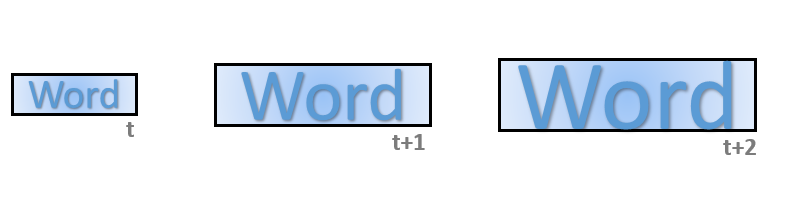
\includegraphics[scale=1]{img/wc_dinamiche/new_word.png}}
\caption[Esempio di parola che compare in $\Gamma^{k}$ ma non in $\Gamma^{k-1}$. In figura � illustrato lo stato della parola in 3 istanti consecutivi.]{Esempio di parola che compare in $\Gamma^{k}$ ma non in $\Gamma^{k-1}$. In figura � illustrato lo stato della parola in 3 istanti consecutivi.}
\label{fig:new_word}
\end{figure}
\item $w_{i} \in S$: caso opposto al precedente, ovvero $w_{i}$ compare solo in $\Gamma^{k-1}$ con un punteggio pari a $\rho_{i}^{k-1}$, per cui si assume che essa avr� un punteggio pari a 0 in $\Gamma^{k}$. Poich� tra $\Gamma^{k-1}$ e $\Gamma^{k}$ ci sono $N$ frame, il punteggio viene decrementato, ad ogni frame, di una quantit� pari a $\dfrac{\rho_{i}^{k-1}}{N+1}$. Come nel caso precedente, la dimensione del rispettivo bounding box viene opportunamente modificata ad ogni frame in base al punteggio corrente della parola (figura \ref{fig:disapp_word}).
\begin{figure}
\centering
{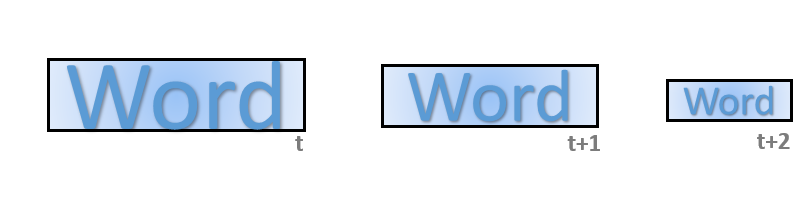
\includegraphics[scale=1]{img/wc_dinamiche/disapp_word.png}}
\caption[Esempio di parola che compare in $\Gamma^{k-1}$ ma non in $\Gamma^{k}$. In figura � illustrato lo stato della parola in 3 istanti consecutivi.]{Esempio di parola che compare in $\Gamma^{k-1}$ ma non in $\Gamma^{k}$. In figura � illustrato lo stato della parola in 3 istanti consecutivi.}
\label{fig:disapp_word}
\end{figure}
\item $w_{i} \in P$: � il caso pi� complesso dei tre. Il termine $w_{i}$ compare in entrambi i layout. Indicati con $\rho_{i}^{k-1}$ il punteggio di $w_{i}$ in $\Gamma^{k-1}$, con $\rho_{i}^{k}$ il punteggio di $w_{i}$ in $\Gamma^{k}$ e con $\Delta_{\rho_{i}}^{k,k-1} = \vert\rho_{i}^{k}-\rho_{i}^{k-1}\vert$ la differenza in valore assoluto tra i due punteggi, se:
\begin{itemize}
\item $\rho_{i}^{k} < \rho_{i}^{k-1} $, il peso di $w_{i}$ viene decrementato di $\dfrac{\Delta_{\rho_{i}}^{k,k-1}}{N+1}$ ad ogni frame;
\item $\rho_{i}^{k} > \rho_{i}^{k-1} $, il peso di $w_{i}$ viene incrementato di $\dfrac{\Delta_{\rho_{i}}^{k,k-1}}{N+1}$ ad ogni frame;
\end{itemize}
In base al punteggio corrente, ad ogni frame la dimensione del rispettivo bounding box di $w_{i}$ viene opportunamente aggiornata. Ovviamente, il peso rimane invariato nel caso in cui il punteggo non cambia tra un disegno e l'altro. \\ 
Inoltre, in questo caso, le parole vengono anche traslate, quindi le posizioni dei rispettivi bounding box variano. Siano dunque:
\begin{itemize}
\item $\tau_{i}^{k-1}=(x_{i}^{k-1},y_{i}^{k-1})$ il centro di $w_{i} $ in $\Gamma^{k-1}$;
\item  $\tau_{i}^{k}=(x_{i}^{k},y_{i}^{k})$ il centro di $w_{i} $ in $\Gamma^{k}$;
\item $\delta_{\tau_{i}}^{k,k-1} = \vert\vert \tau_{i}^{k} - \tau_{i}^{k-1} \vert\vert$ la distanza tra $\tau_{i}^{k}$ e $\tau_{i}^{k-1}$;
\end{itemize}
Ad ogni frame, il bounding box viene traslato, in valore assoluto, di una quantit� pari a $\dfrac{\delta_{\tau_{i}}^{k,k-1}}{N+1}$. La direzione dello spostamento dipende dal relativo posizionamento di $\tau_{i}^{k-1}$ in $\Gamma^{k-1}$ e di $\tau_{i}^{k}$ in $\Gamma^{k}$. Abbiamo in generale quattro casi diversi, come indicato in figura \ref{fig:morphcommon}.
\begin{figure}
\centering
\subfigure[]
{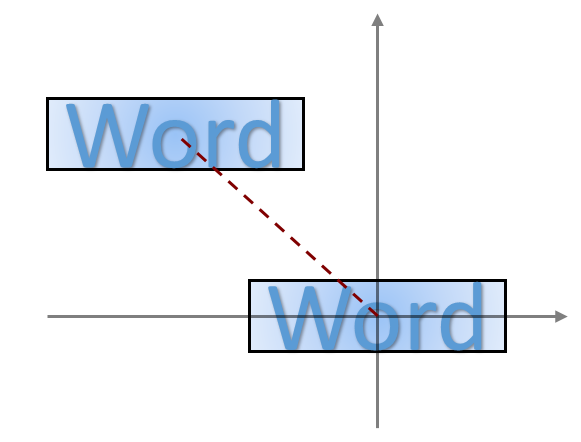
\includegraphics[scale=0.7]{img/wc_dinamiche/morph_4.png}}
\hspace{5mm}
\subfigure[]
{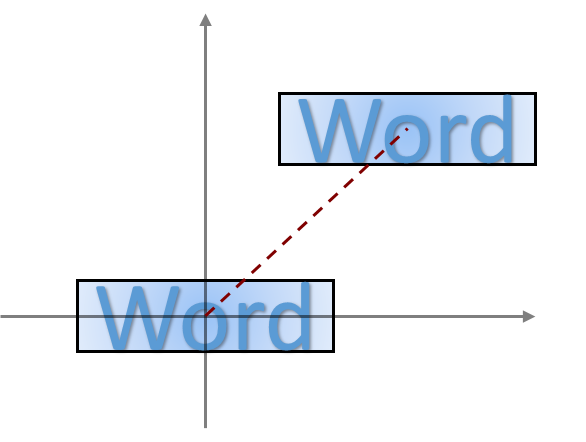
\includegraphics[scale=0.7]{img/wc_dinamiche/morph_1.png}}
\hspace{5mm}
\vspace{10mm}
\subfigure[]
{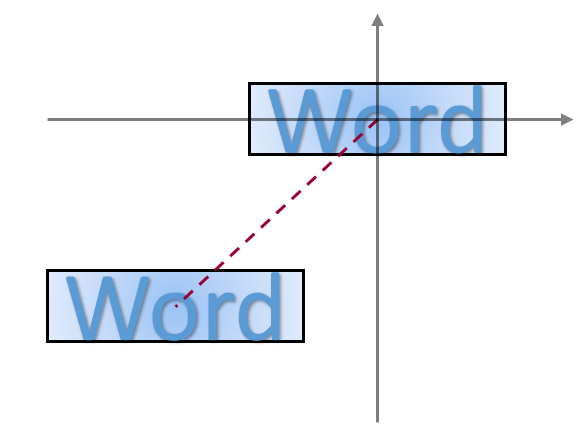
\includegraphics[scale=0.7]{img/wc_dinamiche/morph_3.png}}
\hspace{5mm}
\subfigure[]
{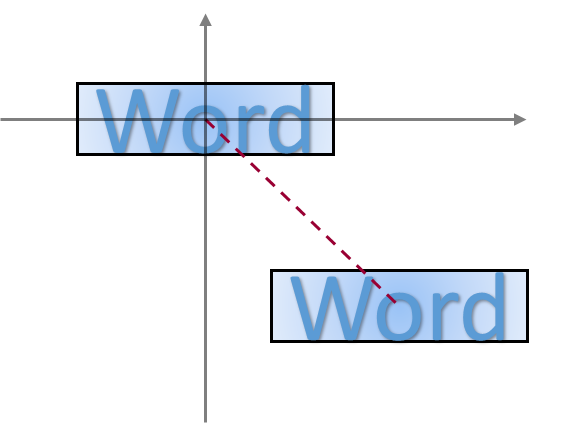
\includegraphics[scale=0.7]{img/wc_dinamiche/morph_2.png}}
\caption[Morphing delle parole comuni a $\Gamma_{i}^{k-1}$ e $\Gamma_{i}^{k}$.]{Morphing delle parole comuni a $\Gamma_{i}^{k-1}$ e $\Gamma_{i}^{k}$. Al centro c'� $\Gamma_{i}^{k-1}$, mentre $\Gamma_{i}^{k}$ pu� trovarsi in uno dei quattro quadranti.}
\label{fig:morphcommon}
\end{figure}
\end{enumerate}
Per quanto riguarda il colore delle parole, si considera il modello di colori RGB (Red, Green, Blue), secondo cui un'immagine pu� essere scomposta in tre colori principali, cio� rosso, verde e blu. Ogni colore � espresso da un intero compreso in $[0,255]$, che � l'intervallo che rappresenta lo spettro dei colori dal nero (valore pari a $0$) al bianco (valore pari a $255$). Ne segue quindi che ogni parola assume un colore dato dalla combinazione di tre interi. La trasformazione da un colore ad un altro viene gestito in modo indipendente per le tre componenti del colore. Dunque, le considerazioni che seguono valgono per ognuna delle componenti del colore.

Come sopra, siano dati due disegni consecutivi $\Gamma^{k-1}$ e $\Gamma^{k}$, intervallati da $N$ frame, e siano dati due interi $x$ e $y$, rappresentanti la stessa componente (rosso, verde o blu) di un colore, rispettivamente in $\Gamma^{k-1}$ e in $\Gamma^{k}$. Volendo raggiungere il valore di $y$ a partire da $x$, la variazione (incremento o decremento, a seconda dei casi) di colore ad ogni frame � pari a $\Delta(x,y) = \ceil[\bigg]{\dfrac{\vert x - y \vert}{N+1}} $. \\  Dunque, data una parola $w_{i}$, si hanno i seguenti tre casi:
\begin{enumerate}
\item $w_{i} \in C$: $w_{i}$ compare solo in $\Gamma^{k}$, con colore espresso dall'intero $y$. Poich� $w_{i}$ non � presente in $\Gamma^{k-1}$, si pu� assumere che, per raggiungere l'intero $y$, il valore $x$ di $w_{i}$ sia inizialmente pari a $255$, valore che rappresenta il bianco (che � lo sfondo della zona di disegno). In altre parole, ad ogni frame, si effettua un  decremento pari a $\Delta(x,y) = \ceil[\bigg]{\dfrac{x-y}{N+1}}$, dove $x=255$.
\item $w_{i} \in S$: $w_{i}$ compare solo in $\Gamma^{k-1}$, con  colore espresso dall'intero $x$. In maniera opposta al caso precedente, si parte da $x$ e si vuole raggiungere l'intero $255$. L'incremento, ad ogni frame, � $\Delta(x,y) = \ceil[\bigg]{\dfrac{y-x}{N+1}}$, dove $y=255$.
\item $w_{i} \in P$: $w_{i}$ compare in $\Gamma^{k-1}$ con colore dato dall'intero $x$ e in $\Gamma^{k}$ con colore dato dall'intero $y$. Per passare da $x$ a $y$, si considerano due casi:
\begin{itemize}
\item se $x<y$, allora l'incremento, ad ogni frame, � $\ceil[\bigg]{\dfrac{y\,-\,x}{N\,+\,1}}$;
\item se $x>y$, allora il decremento, ad ogni frame, � $\ceil[\bigg]{\dfrac{x\,-\,y}{N\,+\,1}}$;
\end{itemize}
\end{enumerate} 
Inoltre, poich� viene usata la parte intera superiore, la variazione minima di colore in ogni frame � pari ad $1$. Ci� significa che, una volta raggiunto il valore cercato (cio� $y$), il colore non varia pi�. 
\onehalfspacing

%%CAPITOLO 3: =======================================

\chapter{Implementazione e sperimentazione}\label{ch:impl_test}
L'architettura del sistema e la fase di sperimentazione sono esposte in questo capitolo.
\\ \\
La sezione \ref{sec:arch} spiega, a grandi linee, i dettagli implementativi degli algoritmi presentati nel precedente capitolo, facendo uso di class diagram per descrivere i moduli funzionali che compongono il sistema. La sezione \ref{sec:test} riporta invece i test eseguiti: dapprima vengono descritte le metriche utilizzate, poi i risultati ottenuti sono illustrati e analizzati con l'ausilio di figure e tabelle.
\section{Architettura del sistema}\label{sec:arch}
Il sistema � stato scritto interamente con il linguaggio di programmazione \textit{Java} in ambiente \textit{Eclipse}.

La word cloud viene generata a partire da un file di testo (formato \textit{.txt}) in input. Tuttavia, il software � dotato di una classe, \texttt{SrtFileCleaner}, la quale permette di ricevere in input un file di testo in formato \textit{.srt}, che � la rappresentazione di un generico sottotitolo con relativi timestamp, e lo ripulisce, in modo da ottenere un semplice file di testo. Il supporto a questo tipo di file � utile perch� la word cloud dinamica si pu� creare a partire da video che contengono il relativo sottotitolo (ad esempio, a partire dai video di YouTube). 

Come descritto nel capitolo precedente, ogni fase pu� essere svolta da pi� algoritmi. L'utilizzo del pattern \textbf{Strategy}\cite{gof}, rende l'architettura parametrica rispetto a tali algoritmi e consente loro di essere intercambiabili. Ci�, inoltre, riduce notevolmente la probabilit� di introdurre errori nel caso si vogliano aggiungere nuovi algoritmi o modificare quelli gi� implementati.

Il file di testo viene elaborato opportunamente in base al numero di campionamenti (istanti di generazione della word cloud) scelto dall'utente e in base al numero di parole da visualizzare (classe \texttt{Document}). L'elaborazione del testo crea le strutture dati (lista delle parole estratte e conteggio delle co-occorrenze tra le parole) che costituiscono l'input dell'algoritmo di calcolo della similarit�. 

Calcolate le parole e le loro similarit�, si crea il grafo delle parole. Ogni grafo viene salvato su una lista di dimensione uguale al numero di campionamenti del testo. Ciascun elemento di tale lista rappresenta il parametro dell'algoritmo di layout che realizza il disegno (implementazione dell'interfaccia \texttt{LayoutStrategy}). Inoltre, ogni algoritmo di layout mantiene un riferimento al disegno precedente, in modo da consentire la preservazione della mappa mentale tra layout consecutivi (vedi paragrafo \ref{subsec:layoutdin}). I disegni (istanze di tipo \texttt{LayoutResult}) vengono quindi salvati su una lista di dimensione pari al numero di campionamenti del testo. 

L'algoritmo K-means++, per ogni elemento della lista dei layout, esegue il clustering delle parole. La classe \texttt{ClusterColorHandler} invoca l'algoritmo di clustering e, inoltre, avendo il riferimento al cluster precedente, gestisce le variazioni dei cluster tra due disegni successivi.

La dinamicit� viene gestita dall'algoritmo di morphing descritto nel precedente capitolo: viene creata una lista di oggetti \texttt{LayoutResult} di dimensione pari al numero di frame scelti. Il metodo \texttt{setFrames(int frames)} permette all'utente di scegliere il numero di frame desiderato tra un layout ed un altro.

La variazione graduale dei colori, tra un frame e l'altro, � realizzata dalla classe \texttt{SimpleColorMorphing}, la quale calcola le variazioni dei colori e assegna, ad ogni frame, il giusto colore alle parole.

Terminata la fase di logica applicativa, viene visualizzata la word cloud dinamica con l'utilizzo di una semplice interfaccia grafica.

\subsection{Estrazione keywords e calcolo similarit�}
 
L'estrazione delle parole e il calcolo delle similarit�, come abbiamo visto nel paragrafo \ref{wc_din:word_ext}, prevede una fase iniziale di preprocessing dell'input. Questa fase � stata realizzata con l'ausilio del toolkit open source \textit{Apache OpenNLP}\cite{opennlp}, basato su tecniche di Machine Learning per l'elaborazione del linguaggio naturale, che consente l'esecuzione dei diversi passaggi che elaborano in modo adeguato il testo in input, al fine di creare le strutture dati necessarie all'algoritmo di estrazione delle keywords. Dunque, grazie ai servizi forniti dal toolkit, vengono eseguiti il rilevamento delle frasi, la suddivisione del testo in token, il processo di stemming e la rimozione delle stop word. Per ciascuna di queste fasi si utilizzano dei modelli (forniti dalla libreria) per l'elaborazione della lingua inglese, ma anche altre lingue sono supportate. 

L'elaborazione del testo, con conseguente estrazione delle keywords, � gestita dalla classe \texttt{Document}, la cui generica istanza ha diversi attributi (figura \ref{class:doc}):
\begin{itemize}
\item il testo da elaborare (variabile \texttt{text});
\item l'algoritmo di rilevamento delle frasi (variabile \texttt{sentenceDetector}); 
\item il tokenizer (variabile \texttt{tokenizer}); 
\item l'algoritmo di stemming (variabile \texttt{stemmer});
\item la lista delle stop word (variabile \texttt{stopWords}).
\end{itemize} 
Nella nostra implementazione l'algoritmo di stemming utilizzato � il Porter Stemmer, fornito dalla libreria. \\ Il metodo che elabora il testo � \texttt{parse()}, il quale predispone in modo opportuno, tramite i parametri del costruttore, la lista delle parole da cui l'algoritmo di ranking estrarr� le parole pi� rilevanti. 
\begin{figure}
\centering
{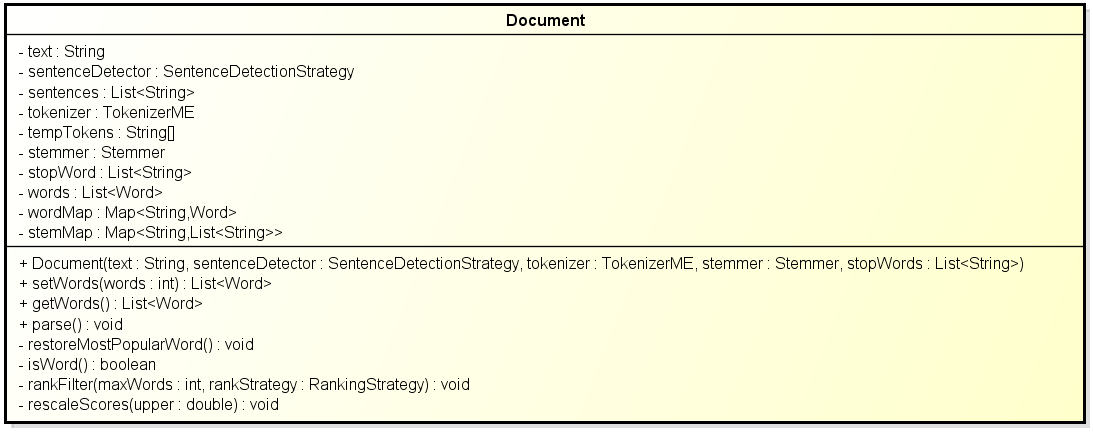
\includegraphics[scale=0.6]{img/impl_test/class_doc.png}}
\caption[Class diagram delle classe  \texttt{Document}.]{Class diagram delle classe  \texttt{Document}.}
\label{class:doc}
\end{figure}
Il ranking e la conseguente estrazione delle parole � quindi gestita dal metodo \texttt{rankFilter(int maxWords,RankingStrategy rankStrategy)}, i cui parametri sono il numero di parole da estrarre e l'algoritmo di ranking. Attraverso il parametro \texttt{rankStrategy} viene invocato il metodo \texttt{rank(Document document)}, che esegue l'effettiva classificazione delle parole. Tale metodo � dichiarato nell'interfaccia \texttt{RankingStrategy} ed � realizzato dalle classi che implementano \texttt{RankingStrategy}, le quali rappresentano i diversi algoritmi di estrazione delle keywords descritti nel precedente capitolo (vedi figura \ref{strategy:rank}). 
\begin{figure}
\centering
{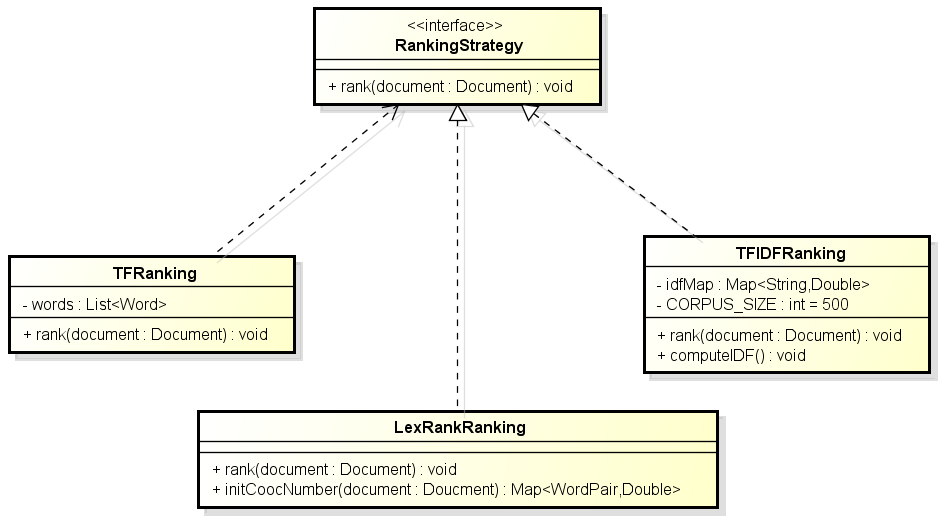
\includegraphics[scale=0.7]{img/impl_test/rank_strategy.png}}
\caption[Classi coinvolte nell'estrazione delle parole.]{Classi coinvolte nell'estrazione delle parole. Nell'implementazione dell'algoritmo TF-IDF, � stato usato il corpus Brown\cite{wiki:browncorpus}.}
\label{strategy:rank}
\end{figure}

Ogni parola � rappresentata da un'istanza della classe \texttt{Word}, che gestisce diverse caratteristiche di una parola, tra cui la radice, il punteggio e le sue variazioni, la lista di frasi in cui essa compare ecc... (figura \ref{class:word}). 
\begin{figure}
\centering
{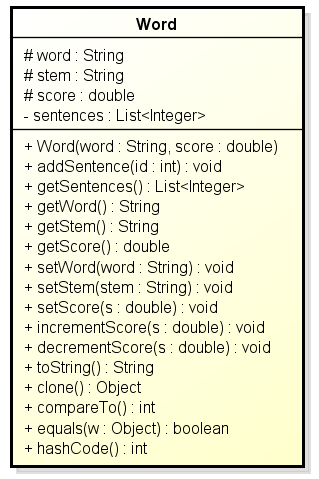
\includegraphics[scale=1]{img/impl_test/class_word.png}}
\caption[Class diagram delle classe \texttt{Word}.]{Class diagram delle classe  \texttt{Word}.}
\label{class:word}
\end{figure}

Una volta estratte le keywords, si procede al calcolo della similarit�, tramite uno degli algoritmi di similarit� definiti in precedenza. Si utilizza un approccio parametrico come per gli algoritmi di ranking (figura \ref{strategy:simil}).
\begin{figure}
\centering
{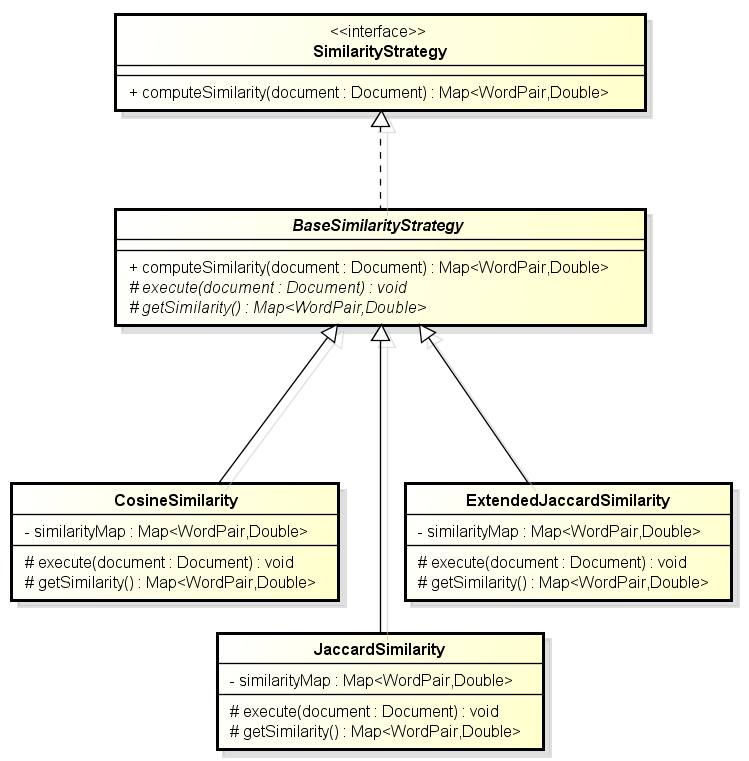
\includegraphics[scale=0.8]{img/impl_test/simil_strategy.png}}
\caption[Classi coinvolte nel calcolo della similarit� tra parole.]{Classi coinvolte nel calcolo della similarit� tra parole.}
\label{strategy:simil}
\end{figure}

\subsection{Creazione word cloud dinamica}
\subsubsection{Layout}
Ottenute la lista delle parole pi� rilevanti e la similarit� a coppie, si procede con la costruzione del grafo delle parole tramite la classe \texttt{WordGraph}, il cui costruttore ha come parametri proprio la lista delle parole e la mappa delle similarit� tra coppie di parole. Gli algoritmi di layout creano il disegno a partire da un oggetto \texttt{WordGraph} e salvano tutte le relative informazioni in un'istanza di \texttt{LayoutResult}. I servizi comuni tra le classi che effettivamente realizzano gli algoritmi sono esposti nella classe astratta \texttt{BaseLayoutStrategy}. In particolare, si hanno i seguenti metodi:
\begin{itemize}
\item \texttt{layout(WordGraph wordGraph)}, che inizializza alcune variabili di utilit�, per poi chiamare il metodo astratto \texttt{execute()}, il quale a tempo di esecuzione sar� ovviamente concreto e verr� eseguito a seconda del tipo effettivo di \texttt{LayoutStrategy};
\item \texttt{createResult()}, il quale crea un oggetto di tipo \texttt{LayoutResult} e lo salva nella variabile \texttt{lastResult}. Questo riferimento sar� la chiave per il mantenimento della mappa mentale nel passaggio da una word cloud ad un'altra;
\item \texttt{createBoundingBoxes()} associa, ad ogni parola contenuta nella lista \texttt{words} (contenente oggetti di tipo \texttt{Word}), il relativo bounding box, che non � altro che un oggetto \texttt{Rectangle}. Questa mappatura viene salvata nella variabile \texttt{wordPositionsMap}. Per generare il bounding box, Java consente di estrarre il bounding box di una sequenza di caratteri tramite il toolkit Graphics2D. La dimensione del bounding box viene quindi opportunamente scalata in base al relativo punteggio  di ciascuna parola.
\end{itemize}
\begin{figure}
\centering
{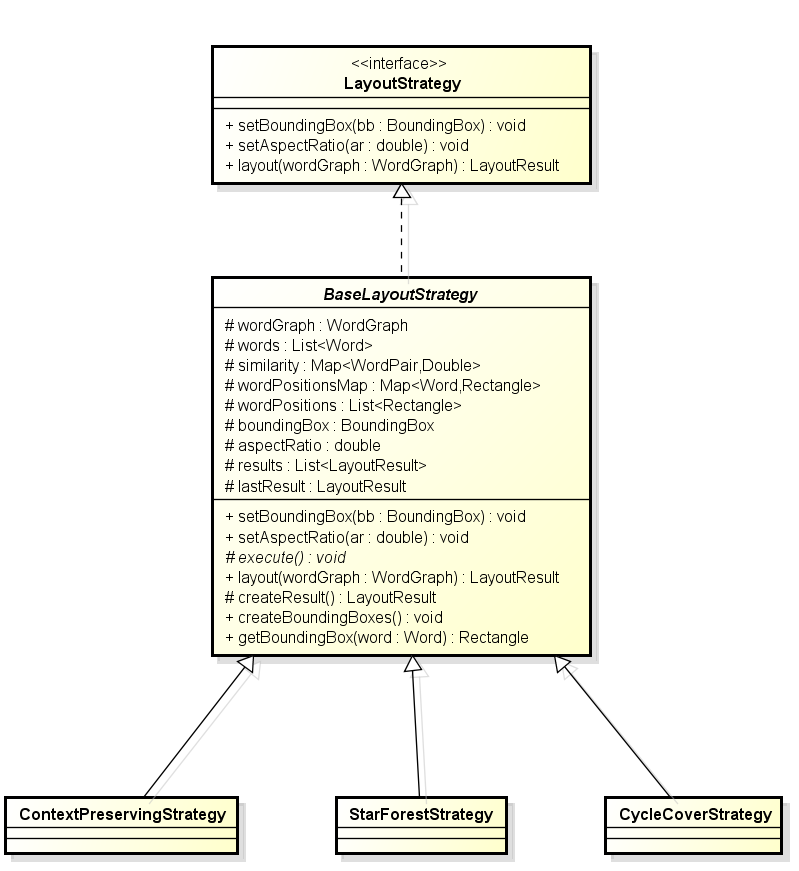
\includegraphics[scale=0.8]{img/impl_test/layout_strategy.png}}
\caption[Classi coinvolte nella creazione della word cloud.]{Classi coinvolte nella creazione della word cloud.}
\label{strategy:layout}
\end{figure}
La coerenza della mappa mentale, come detto, viene rispettata grazie al riferimento all'ultimo disegno realizzato, denotato dalla variabile \texttt{lastResult}. Tale variabile viene ereditata dallo specifico algoritmo di layout ed � gestita in modo opportuno nell'implementazione della procedura force directed descritta nel paragrafo \ref{subsec:layoutdin}. Tale procedura viene eseguita subito dopo l'applicazione dello scaling multidimensionale al grafo delle parole, che colloca sul piano le parole in base alla loro similarit�. Il metodo force directed, grazie al riferimento all'ultimo layout, riesce a ricavare le parole in comune tra i due layout. Per ognuna di queste parole, viene calcolata la distanza tra la vecchia e la nuova posizione, dunque si applica una forza attrattiva proporzionale al punteggio della parola nel layout corrente. Il numero massimo di iterazioni � 1000. \\ Di seguito � riportato lo pseudocodice della procedura force directed utilizzata.
\begin{algorithm}
\label{iter_algorithm}
\begin{algorithmic}[1]
\Procedure{ForceDirected\textendash Iteration}{}
\State siano $\Gamma_{i-1}$ il layout precedente, $\Gamma_{i}$ il layout corrente e sia $W$ l'insieme delle parole comuni a $\Gamma_{i-1}$ e $\Gamma_{i}$;
\Repeat
\For{\textbf{each} parola $w$ \Pisymbol{psy}{206} $W$ }
\State sia $\tau_{i-1} \gets $ posizione di $w$ in $\Gamma_{i-1}$;
\State sia $\tau_{i} \gets$ posizione di $w$ in $\Gamma_{i}$;
\State $\rho_{i} \gets$ punteggio di $w$ $\Gamma_{i}$;
\State $\delta \gets \textsc{attractiveforce}$($\tau_{i-1}$,$\tau_{i}$,$\rho_{i}$);
\State muovi $r_{i}$ in direzione di $r_{i-1}$ di una quantit� pari a $\delta$;
\EndFor
\Until{equilibrio raggiunto OR iterazioni massime effettuate;}
\EndProcedure
\end{algorithmic}
\caption{Avvio iterazione.}
\end{algorithm}
\begin{algorithm}
\label{att_force}
\begin{algorithmic}[1]
\Procedure{AttractiveForce($\tau_{i-1}$,$\tau_{i}$,$\rho_{i}$)}{}
\State $P=(x,y) \gets$ punto di coordinate $x$ e $y$ corrispondenti alle distanze dei centri di $\tau_{i-1}$ e $\tau_{i}$;
\State $\bar{P} \gets$  normalizzazione di $P$;
\State \Return $\bar{P}$ scalato di una quantit� proporzionale a $\rho_{i}$;
\EndProcedure
\end{algorithmic}
\caption{Calcolo forza attrattiva.}
\end{algorithm}
\subsubsection{Clustering}
L'esecuzione dell'algoritmo di clustering K-means++ avviene per ciascun oggetto di tipo \texttt{WordGraph}. Per calcolare il corretto numero di cluster, viene avviato pi� volte l'algoritmo a partire da $k = \sqrt{n/2}$, incrementando $k$ di una unit� ad ogni iterazione. Poi si esegue il confronto tra clustering successivi per selezionare quello migliore. 

L'algoritmo viene eseguito dalla classe \texttt{ClusterColorHandler} (vedi figura \ref{class:clusterhandler}), mediante l'invocazione del metodo \texttt{initialize(WordGraph wordGraph, ClusterResult prevResult)}. Il cluster prodotto � referenziato dalla variabile \texttt{clustering}, il cui tipo � \texttt{ClusterResult}, struttura dati che contiene tutte le informazioni relative al cluster. Ad ogni cluster � associato un intero, il quale corrisponde all'indice di un elemento dell'array dei colori da assegnare alle parole del cluster (variabile \texttt{colorSequence}). Il metodo \texttt{getColor(Word w)}, quindi, consente di restituire il colore della parola \texttt{w} tramite l'indice associato al cluster di \texttt{w}. Il metodo \texttt{updateClusters(ClusterResult prevResult)}, gestisce invece la variazione dei cluster tra due layout successivi, per mezzo dei seguenti passaggi: 
\begin{itemize}
\item vengono calcolati i valori di similarit� tra i cluster del layout precedente (variabile \texttt{prevResult}) e di quello corrente (variabile \texttt{clustering}) tramite l'algoritmo di similarit� che implementa l'interfaccia \texttt{ClusterSimilarityStrategy};
\item viene invocato il metodo \texttt{computeBestPairs(List<ClusterPair> bestPairs)}, il quale salva su una lista le coppie (di interi) con i valori pi� alti;
\item se il numero di cluster, nel layout corrente, � aumentato, allora vengono aggiunte nuove coppie alla lista \texttt{bestPairs}, le quali sono calcolate in base agli interi non ancora assegnati ad alcun cluster. Il numero di coppie aggiunto � uguale a $m-l$, dove $l$ � il numero di cluster del disegno precedente ed $m$ il numero di cluster del disegno attuale; 
\item infine, il cluster corrente viene modificato invocando  \texttt{updateClusters(bestPairs)}, metodo offerto della classe \texttt{ClusterResult}, che esegue l'aggiornamento degli indici dei vari cluster;
\end{itemize}
Al termine, per ciascun oggetto \texttt{WordGraph}, si ottiene un oggetto \texttt{ClusterResult} aggiornato.
\begin{figure}
\centering
{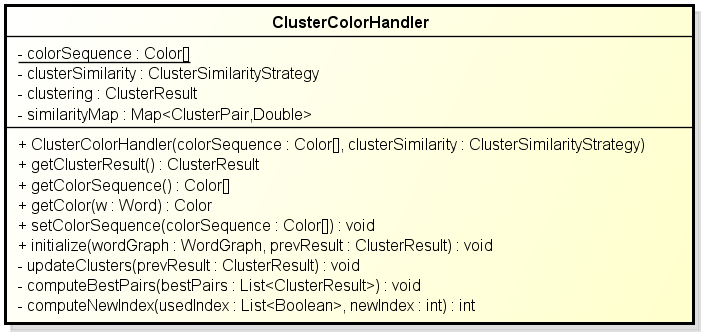
\includegraphics[scale=0.95]{img/impl_test/class_clusterhandler.png}}
\caption[Class diagram della classe \texttt{ClusterColorHandler}.]{Class diagram della classe \texttt{ClusterColorHandler}.}
\label{class:clusterhandler}
\end{figure}

\subsubsection{Morphing}
La dinamicit� � conferita dallo specifico algoritmo di morphing che implementa l'interfaccia \texttt{MorphingStrategy}. Ovviamente, anche in questo caso � possibile estendere facilmente l'architettura con nuovi algoritmi. L'interfaccia definita prevede quindi due metodi: 
\begin{itemize}
\item il primo, \texttt{morph(LayoutResulta resultA)}, prende come parametro un solo layout ed esegue il morphing iniziale, ovvero quello in cui, nella word cloud, compaiono solo nuove parole;
\item il secondo, \texttt{morph(LayoutResulta resultA, LayoutResult resultB)}, prende come parametri due layout consecutivi e ne esegue il morphing. 
\end{itemize}
Questi due metodi estraggono una lista di disegni (oggetti \texttt{LayoutResult}) con le posizioni delle parole via via aggiornate. La dimensione di tale lista � pari al numero di frame scelto tra una word cloud e la successiva, definito dal parametro \texttt{frames} del costruttore dello specifico algoritmo di morphing che estende \texttt{MorphingStrategy}. \\ L'algoritmo di morphing utilizzato � rappresentato dalla classe \texttt{SimpleMorphing}, che implementa diversi metodi, tra cui:
\begin{itemize}
\item \texttt{morphNewWords(int iter)}, il quale, per ogni elemento della lista \texttt{newWords}, incrementa il punteggio ad ogni frame e restituisce una mappa in cui, a ciascuna parola, � associata un rettangolo con le dimensioni aggiornate;
\item \texttt{morphDisappearingWords(int iter)}, il quale, per ogni elemento della lista \\ \texttt{disappearingWords}, decrementa il punteggio ad ogni frame e restituisce una mappa in cui, a ciascuna parola, � associata un rettangolo con le dimensioni aggiornate;
\item \texttt{morphCommonWords(int iter)}, il quale, per ogni elemento della lista \texttt{commonWords}, incrementa o decrementa il punteggio ad ogni frame. Inoltre, viene chiamato il metodo \texttt{handleRects(...)} che, a seconda dei casi (vedi paragrafo \ref{subsec:morphing}), aggiorna le coordinate delle parole. Il metodo restituisce dunque una mappa in cui, a ciascuna parola, � associato un rettangolo con le coordinate e le dimensioni aggiornate.
\end{itemize}
Quindi, una volta terminato il morphing, se $n$ � il numero di frame tra un layout ed un altro, vengono creati $n$ oggetti \texttt{LayoutResult}, che rappresentano i layout aggiornati frame per frame.
\begin{figure}
\centering
{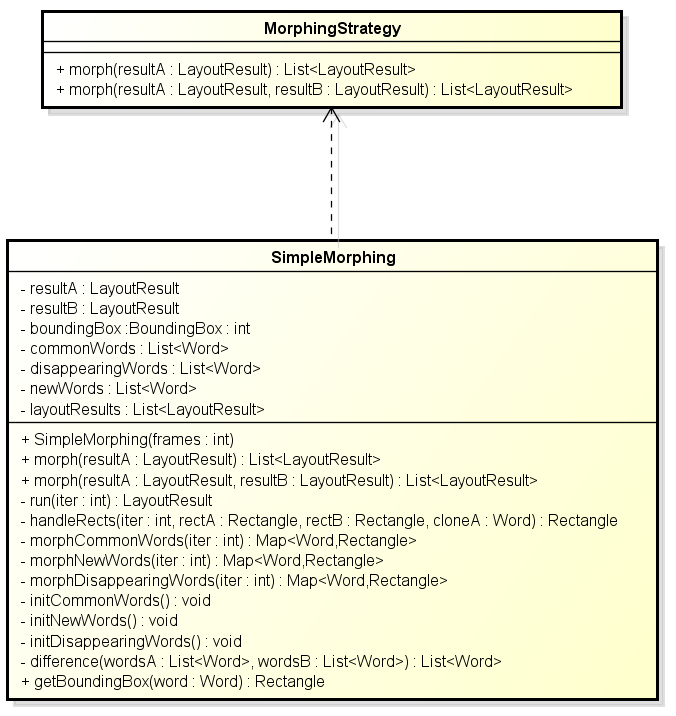
\includegraphics[scale=0.8]{img/impl_test/morph_strategy.png}}
\caption[Classi coinvolte nell'operazione di morphing.]{Classi coinvolte nell'operazione di morphing.}
\label{strategy:morph}
\end{figure}
\\ \\
La variazione del colore da un layout al successivo � invece trattata, con un approccio simile alla classe \texttt{SimpleMorphing}, dalla classe \texttt{SimpleColorMorphing}. La classe \texttt{Color} di Java codifica i colori, nel modello RGB, con interi compresi tra 0 a 255. Come sopra, i metodi \texttt{morphNewWords(...)}, \texttt{morphDisappearingWords(...)} e \texttt{morphCommonWords(...)} applicano il morphing dei colori tra due disegni consecutivi, con la differenza che il tipo restituito � un array di oggetti \texttt{Color} (nel caso dei primi due metodi) o una matrice di oggetti \texttt{Color} (nel caso del terzo metodo). Queste strutture dati vengono restituite alla classe \texttt{DynamicColorHandler}, che si occupa, ad ogni frame, di assegnare il colore esatto a ciascuna parola, tramite il metodo \texttt{getColor(Word w)}, cos� come nella classe \texttt{ClusterColorHandler}.
\subsection{Interfaccia grafica}
La visualizzazione dinamica della word cloud avviene per mezzo di una semplice interfaccia grafica sviluppata con il framework \textit{Swing} di Java. L'interfaccia contiene i bottoni tipici di un qualsiasi player, i quali permettono di avviare la visualizzazione, metterla in pausa, riavviarla, passare direttamente alla successiva word cloud o alla precedente (vedi figura \ref{ex:ui}). 

%I frame della word cloud sono gestiti tramite il layout manager \texttt{CardLayout}, che consente il passaggio da un \texttt{JPanel} (che rappresenta un frame) all'altro in modo continuo, grazie all'utilizzo dei comandi del player.
Sempre in figura \ref{ex:ui} si nota, in basso a sinistra, un grafico a barre (la cui visibilit� si pu� impostare dal men�) contenente le 10 parole pi� importanti ad ogni layout, ordinate in base al relativo punteggio. Tale finestra � stata realizzata tramite la libreria Java \textit{JFreeChart}\cite{JFreeChart}.
\begin{figure}
\centering
\subfigure[]
{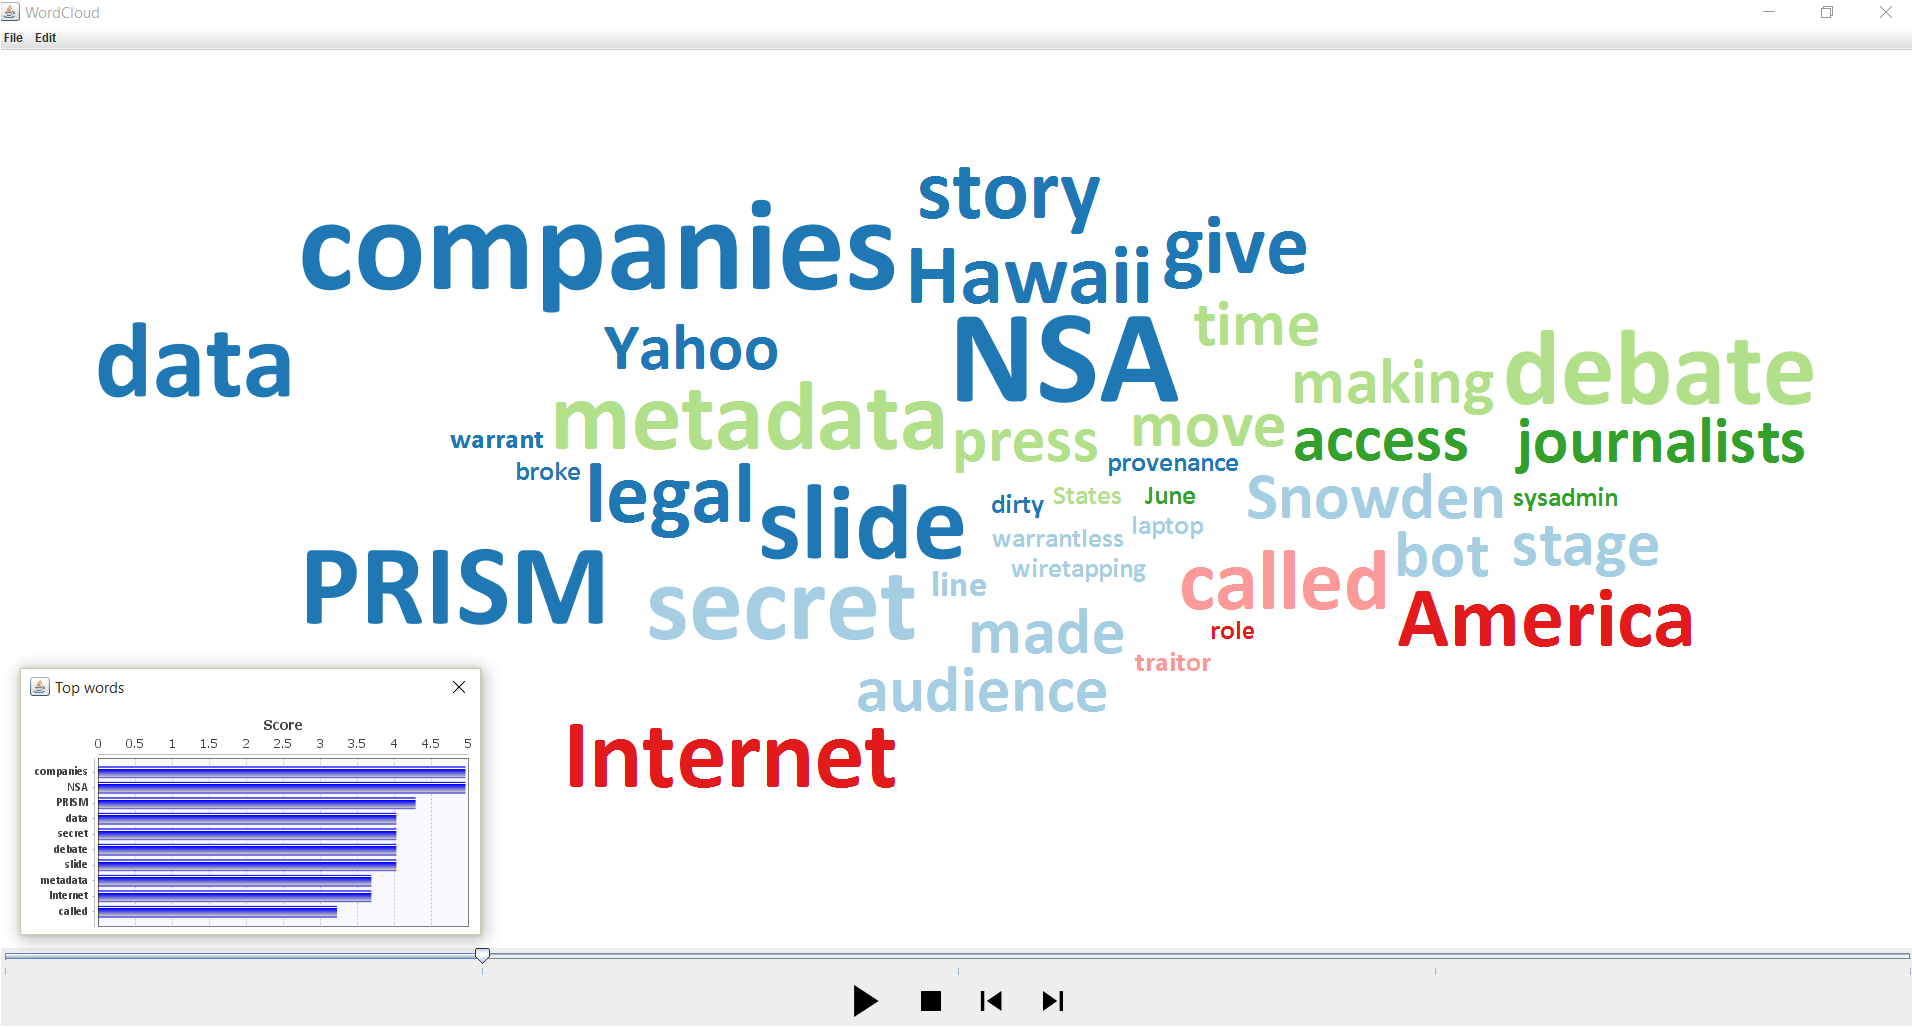
\includegraphics[scale=0.3]{img/impl_test/wordcloud_ui1.png}}
\subfigure[]
{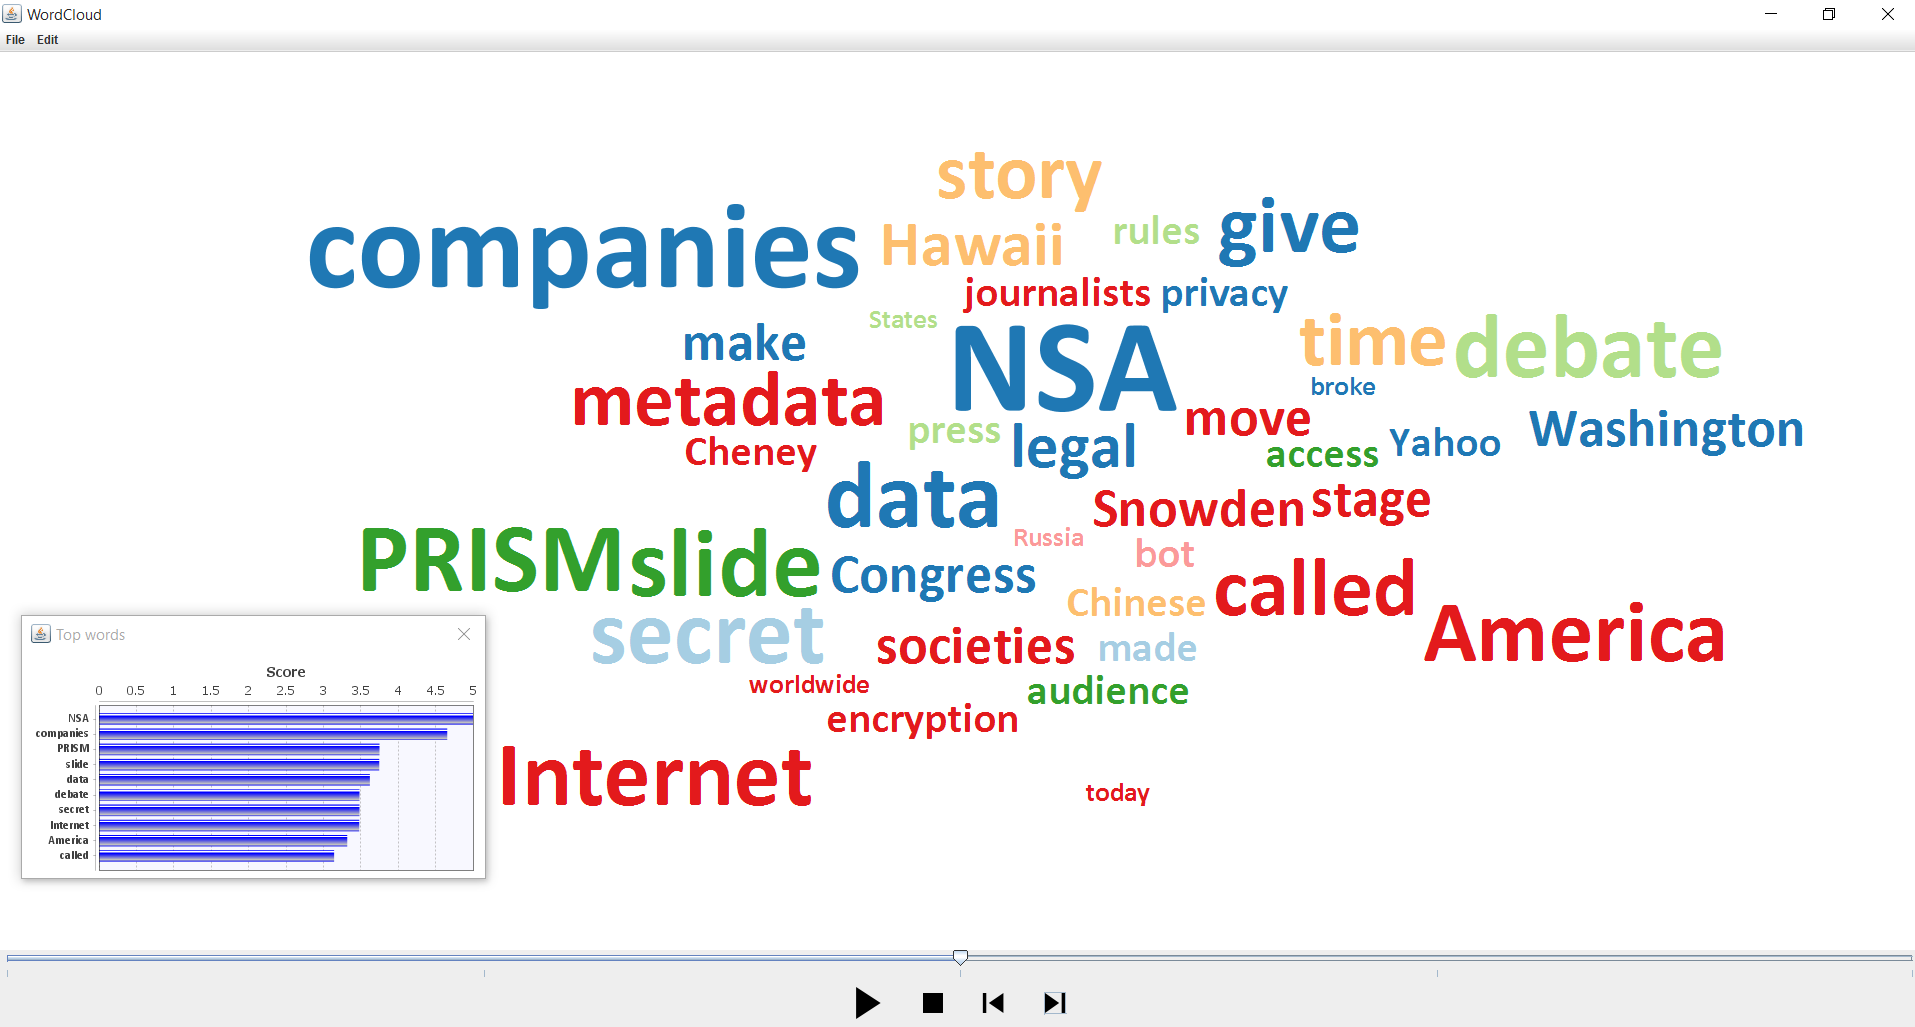
\includegraphics[scale=0.3]{img/impl_test/wordcloud_ui2.png}}
\caption[Esempio di visualizzazione dinamica di una word cloud in due layout successivi.]{Esempio di visualizzazione dinamica di una word cloud in due layout successivi.}
\label{ex:ui}
\end{figure}

\section{Risultati sperimentali}\label{sec:test}
Il sistema � stato testato su un dataset di 200 testi, corrispondenti a discorsi estratti da video della conferenza \textit{TED}\cite{ted}. Le trascrizioni dei video (file di testo \textit{.txt}) sono state ottenute grazie al tool online TED2SRT\cite{ted2srt}. Ogni discorso tratta temi di attualit� e la durata media � di circa 17 minuti. La sperimentazione � stata infine effettuata su un calcolatore con processore Intel i7 2.40Ghz e memoria RAM 8GB. 
\subsection{Metriche adottate}
Gli algoritmi di layout sono stati testati sulla base di diverse metriche. Le metriche tengono conto sia di aspetti quantitativi (compattazione, distanza tra parole correlate semanticamente) che qualitativi (mantenimento della mappa mentale) ed assumono valori compresi nell'intervallo $[0,1]$.

\subsubsection{Distortion metric}
Data una word cloud $\Gamma^{k}$, $k \in \{1,...,K\}$, tale metrica misura la vicinanza geometrica tra parole correlate semanticamente nel disegno. In particolare, siano: 
\begin{itemize}
\item $s_{ij}$ il valore di similarit�, compreso tra $0$ e $1$, tra la parola $w_{i}$ e la parola $w_{j}$ ed estratto dalla matrice di similarit� calcolata con uno degli algoritmi descritti in precedenza;
\item $d_{ij}$ la distanza normalizzata (cio� compresa tra $0$ e $1$) tra la parola $w_{i}$ e la parola $w_{j}$. Essa � calcolata come $d_{ij}=\dfrac{\delta_{ij}}{D}$, dove $\delta_{ij}$ � la distanza minima tra due bounding box, mentre $D$ � la massima distanza possibile nel disegno tra due punti, cio� la diagonale del pi� grande bounding box che contiene la word cloud. In generale, nel calcolo di $\delta_{ij}$, si hanno tre casi (vedi figura \ref{dist_rett}). Se $b_{i}$, $h_{i}$ e $c_{i}$ rappresentano la base, l'altezza e il centro del bounding box di $w_{i}$, allora $\delta_{ij} = \sqrt{\Delta_{x_{ij}}^2 +\Delta_{y_{ij}}^2 }$, dove:
\begin{itemize}
\item la quantit� $\Delta_{x_{ij}} = \max \{{0,\vert c_{x_{i}}-c_{x_{j}}\vert - \dfrac{b_{i}+b_{j}}{2}}\}$ rappresenta la distanza minima sull'asse x;
\item la quantit� $\Delta_{y_{ij}} = \max \{{0,\vert c_{y_{i}}-c_{y_{j}}\vert - \dfrac{h_{i}+h_{j}}{2}}\}$ rappresenta la distanza minima sull'asse y.
\begin{figure}
\centering
\subfigure[Distanza solo sulle ascisse.]
{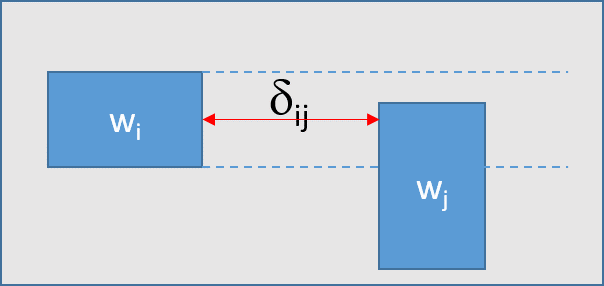
\includegraphics[scale=0.75]{img/impl_test/dist_1.png}}
\hspace{1cm}
\subfigure[Distanza solo sulle ordinate.]
{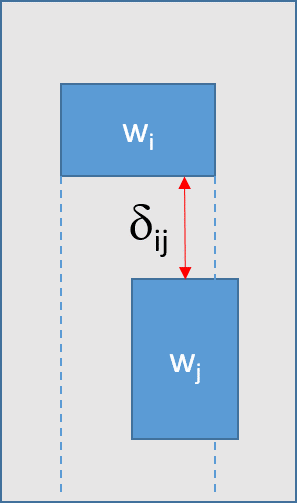
\includegraphics[scale=0.75]{img/impl_test/dist_2.png}}
\subfigure[Distanza su entrambi gli assi.]
{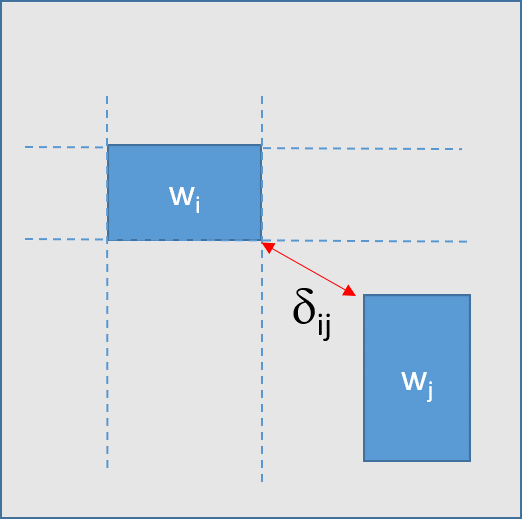
\includegraphics[scale=0.75]{img/impl_test/dist_3.png}}
\caption[Distanza minima tra due parole.]{Distanza minima tra due parole.}
\label{dist_rett}
\end{figure}
\end{itemize}
Per ogni coppia di parole $w_{i}$ e $w_{j}$, dunque, si calcola il coefficiente $c_{ij} = (1-d_{ij})^2$.
\end{itemize}
La misura $S^{k}$ della vicinanza geometrica fra parole correlate semanticamente nel disegno $\Gamma_{k}$ viene quindi calcolata combinando $c_{ij}$ con $s_{ij}$ mediante la seguente formula:
\begin{equation}
S^{k} = \dfrac{\sum \nolimits_{ij} c_{ij}s_{ij}}{\sum \nolimits_{ij} s_{ij}},
\end{equation}
dove $S^{k} \in [0,1]$. Se tale valore � vicino a $1$, allora la distanza geometrica rispecchia la similarit�, altrimenti se tale valore tende a $0$ vale il contrario.
\subsubsection{Coherence metric}
Il mantenimento della mappa mentale tra due disegni consecutivi � calcolato con questa metrica. Dati due disegni consecutivi $\Gamma^{k-1}$ e $\Gamma^{k}$, con $k \in \{2,...,K\}$, indichiamo con
$P = \{w_{1},...,w_{p}\}$ l'insieme delle $p$ parole comuni a $\Gamma^{k-1}$ e $\Gamma^{k}$. Denotiamo con $\sigma(w_{i}^{k},w_{i}^{k-1}, w_{i} \in P$, la variazione di posizione della parola $w_{i}$ nel disegno $\Gamma^{k}$. Sia inoltre $D$ la diagonale del pi� grande bounding box che contiene la word cloud. La metrica � definita come:
\begin{equation}
\vartheta^{k,k-1} = 1 - \dfrac{\sum \limits_{i=1}^p \sigma(w_{i}^{k},w_{i}^{k-1})}{pD}
\end{equation}
Ne segue che:
\begin{enumerate}
\item $\vartheta^{k,k-1} \in [0,1]$;
\item essendo $k \in \{2,...,K\}$, tale misura non � definita per il primo layout. Si pu� dunque assumere che $\vartheta^{1,0}=1$;
\end{enumerate}
\subsubsection{Combination metric}
Per ciascun disegno $\Gamma^{k}, k \in \{1,...,K\}$, sono state calcolate $S^{k}$ e $\vartheta^{k,k-1}$. A questo punto si pu� ottenere una nuova metrica, combinazione lineare delle due metriche appena definite:
\begin{equation}
\nu = \dfrac{1}{K}\sum\limits_{k=1}^K (\alpha S^{k} + \beta\vartheta^{k,k-1})
\end{equation}
dove:
\begin{itemize}
\item $K$ � il numero di word cloud realizzate;
\item $\alpha$ e $\beta$ sono due coefficienti entrambi positivi e tali che $\alpha + \beta=1$;
\end{itemize}
La definizione di questa metrica � utile poich�, come gi� espresso in precedenza, la vicinanza geometrica tra parole maggiormente correlate semanticamente e la preservazione della mappa mentale cosituiscono due obiettivi contrastanti. Con i valori ottenuti da questa metrica, � possibile analizzare gli algoritmi di disegno sulla base di tali parametri e scegliere quindi l'algoritmo adatto in base alle proprie esigenze. 
\subsubsection{Space metric}
L'uso efficiente dell'area di disegno viene racchiusa da questa semplice misura. Si calcola l'area utilizzata come la somma delle aree dei bounding box di ciascuna parola ($\mu$); poi si calcola l'area del bounding box (o dell'inviluppo convesso, detto \textit{convex hull}) che contiene tutte le parole ($\varphi$). La \textbf{compattezza} � definita come $ \gamma = 1 - \dfrac{\mu}{\varphi}$. Se tale valore tende ad $1$, allora si ha un disegno poco compatto, mentre un valore tendente a zero denota un disegno troppo compatto.
\subsubsection{Running time}
Il calcolo del tempo d'esecuzione consiste nel conteggio del tempo  necessario ad eseguire i diversi passaggi nella creazione della word cloud, a partire dall'elaborazione del testo, fino ad arrivare alla generazione dell'interfaccia grafica. Il tempo di esecuzione � stato valutato dunque per:
\begin{itemize}
\item l'elaborazione del testo ed estrazione delle keywords;
\item il calcolo delle similarit�;
\item la creazione della word cloud;
\item l'applicazione della procedura di morphing tra le parole;
\item il clustering e la gestione delle variazioni dei cluster tra una word cloud e l'altra;
\item la gestione delle variazioni dei colori delle parole;
\item la generazione dell'interfaccia grafica;
\item tempo totale di esecuzione.
\end{itemize}
Eccetto per gli ultimi due valori, tutti i tempi sono stati mediati sul numero di campionamenti del testo (pari a $4$).
\subsection{Risultati}
La durata media dei discorsi che compongono il dataset � di circa 17 minuti, per cui si � scelto di creare le word cloud in 4 istanti, in modo da ottenere una prima finestra temporale tra i 4 e i 5 minuti e avere abbastanza parole da estrarre. Inoltre, poich� l'evoluzione della word cloud � dinamica, � bene non visualizzare troppe parole, in modo da non creare confusione all'utente. Per questi motivi, sono state realizzate, per ogni combinazione degli algoritmi utilizzati, tre word cloud da 20, 40 e 60 parole ciascuna.

\subsubsection{Combination metric}
Sono stati calcolati i valori dei tre algoritmi di layout per tutte le combinazioni possibili tra il numero di parole, l'algoritmo di ranking e l'algoritmo di similarit�. Gli andamenti degli algoritmi sono riportati nelle figure delle pagine successive. I valori assunti giacciono su una retta che congiunge due punti, cio� $\alpha=0$, che coincide con la misura della Coherence, e $\alpha=1$, che coincide con la misura della Distortion. In entrambe le metriche, la quantit� $D$, cio� la diagonale del bounding box che contiene la word cloud, � presa come il massimo per ogni coppia $\{$numero di parole,algoritmo di layout$\}$.

Nei grafici si pu� notare come le rette siano crescenti o decrescenti, a seconda dei rispettivi valori della Coherence o della Distortion. Essendo due misure contrastanti, tali rette si intersecano spesso, per cui un algoritmo pu� comportarsi meglio su una metrica rispetto ad un altro algoritmo, e viceversa.

In generale, l'algoritmo che offre le performance migliori � Cycle Cover, superando quasi sempre Star Forest e CPWCV. In particolare, preserva piuttosto bene la mappa mentale, mentre, per quanto riguarda la Distortion, i valori assunti dai vari algoritmi tendono ad essere molto vicini e in ogni caso sono pi� che discreti (confermando i risultati del lavoro di Kobourov et al.\cite{kobourov}). Com'era lecito aspettarsi, i valori pi� alti si osservano nel caso di 20 parole estratte, mentre all'aumentare delle parole i valori decrescono. Star Forest ha un comportamento simile a Cycle Cover, assumendo valori leggermente inferiori sulla Coherence. CPWCV � invece l'algoritmo che, il pi� delle volte, si comporta peggio nella misura della coerenza della mappa mentale. Ci� fa si che le parole tendano a muoversi di pi�, migliorando d'altro canto la Distortion. La retta che rappresenta l'andamento della CPWCV, infatti, ha solitamente un andamento non decrescente.

\begin{figure}
\centering
{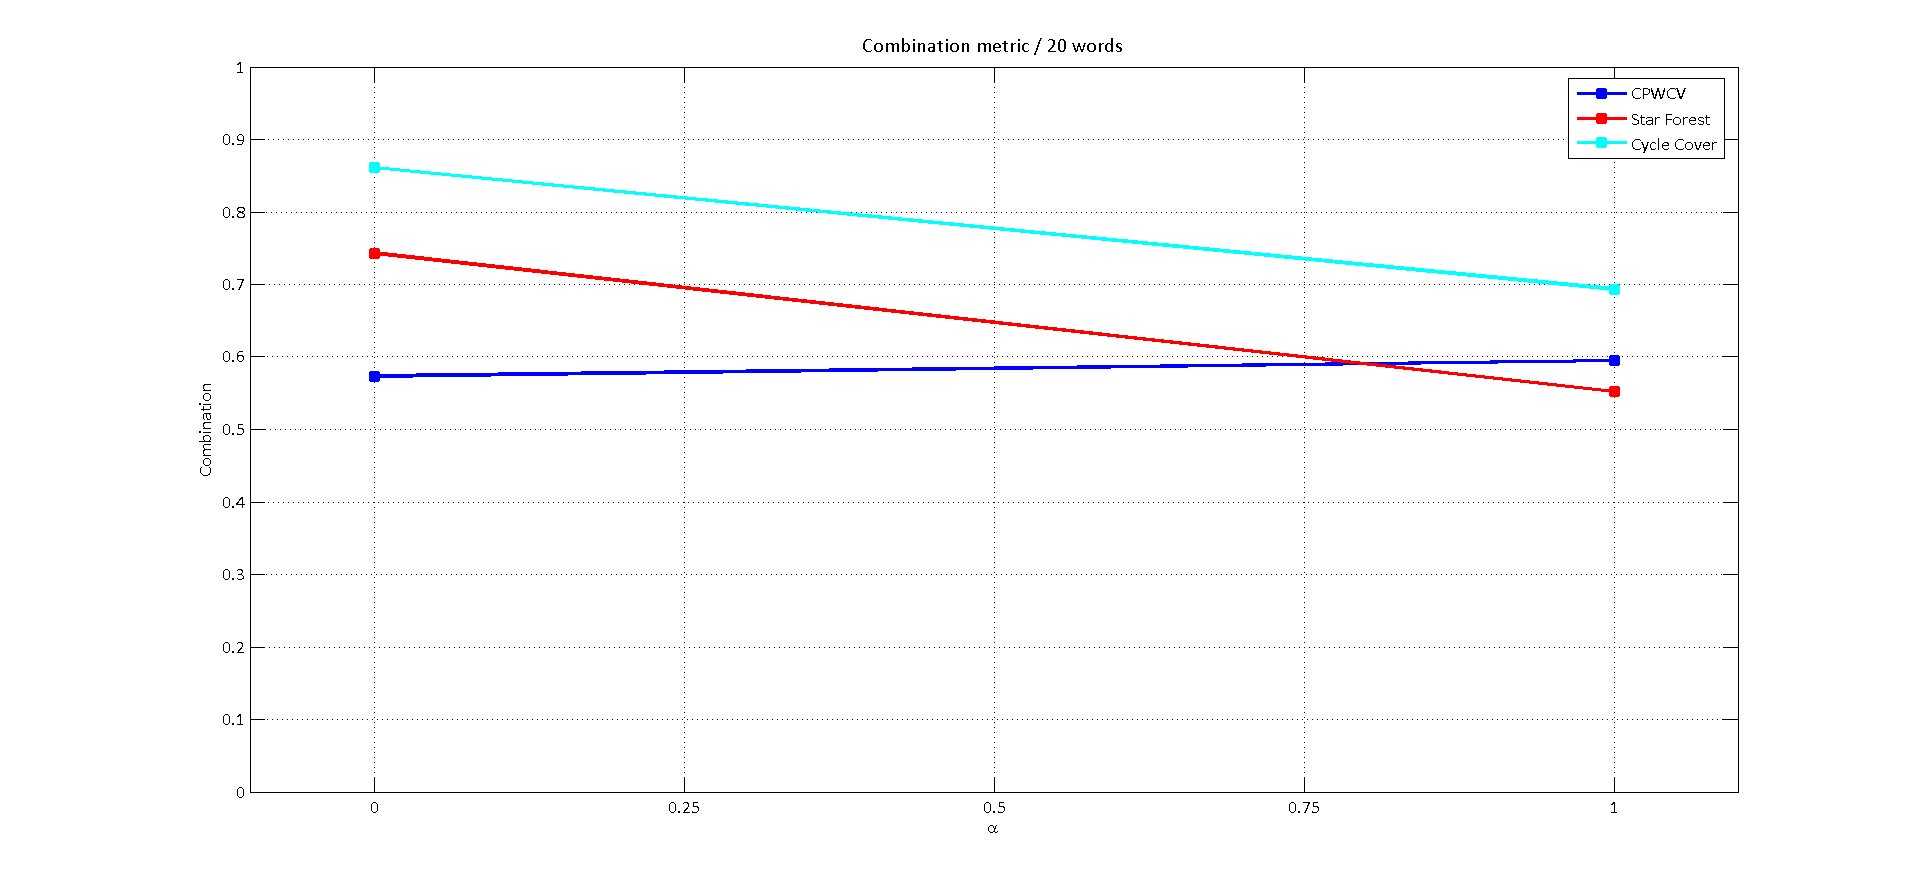
\includegraphics[scale=0.35]{img/impl_test/test_tf_jaccard/figures/combo_20.png}}
\caption{Combination metric: Term Frequency + Jaccard Similarity con 20 parole estratte.}
\label{combo_tf_jaccard_20}
\end{figure}
\begin{figure}
\centering
{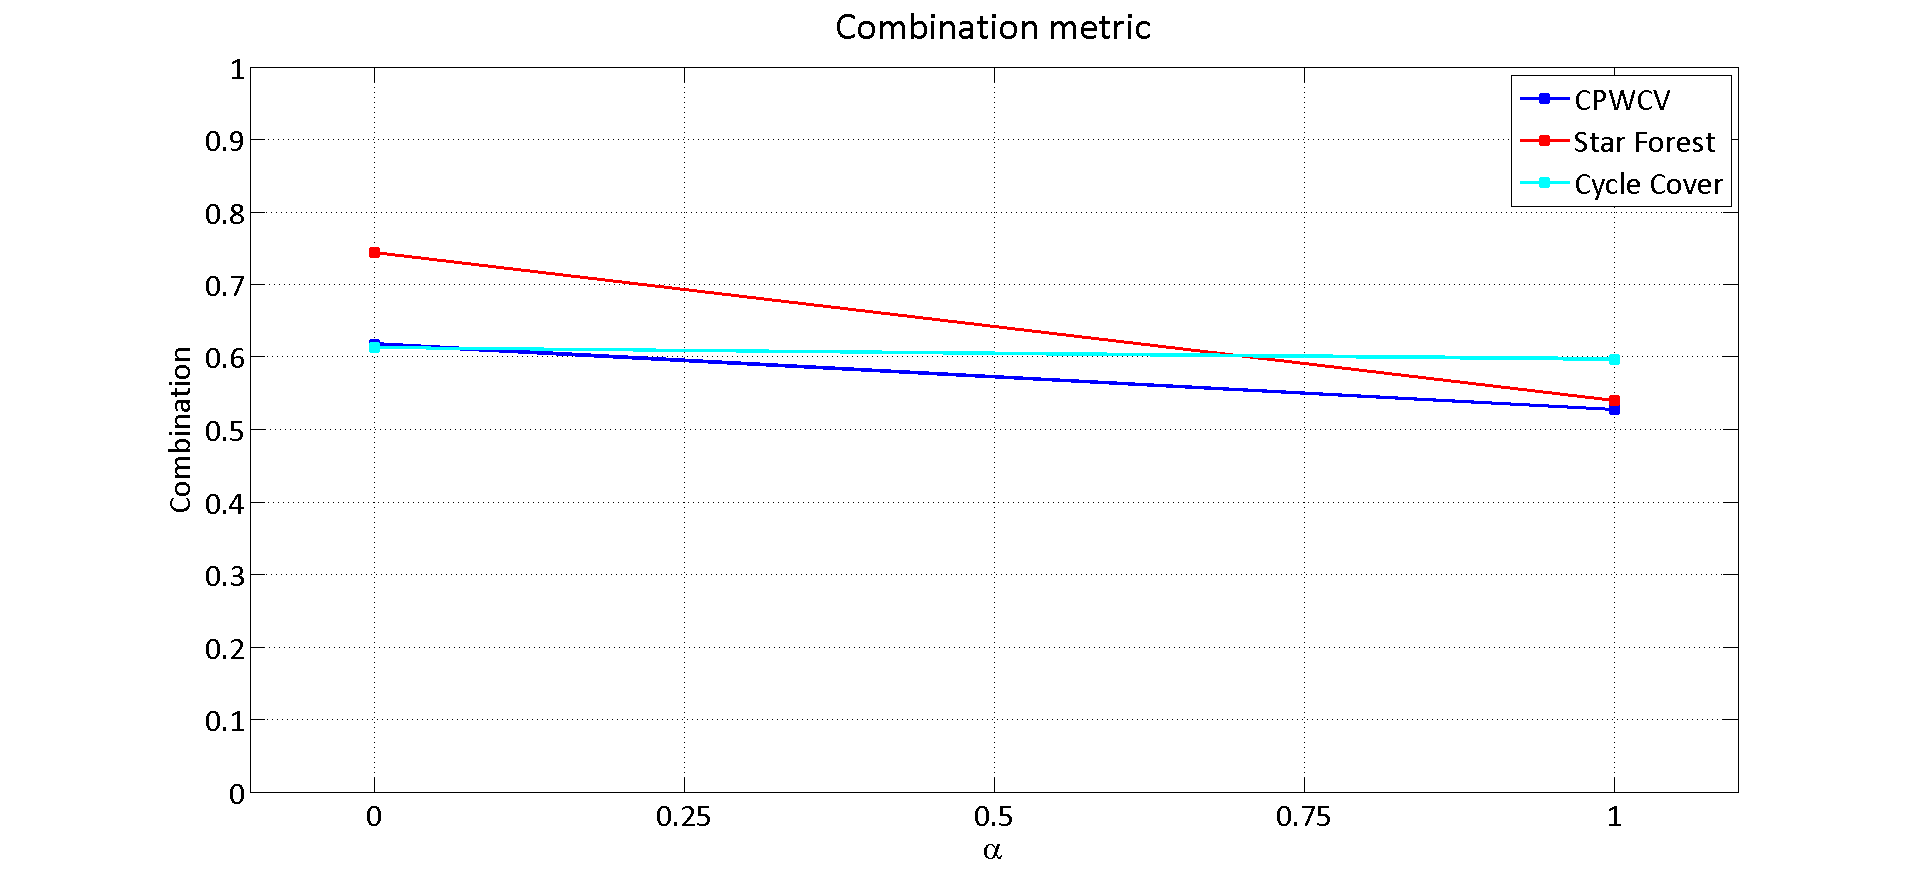
\includegraphics[scale=0.35]{img/impl_test/test_tf_jaccard/figures/combo_40.png}}
\caption{Combination metric: Term Frequency + Jaccard Similarity con 40 parole estratte.}
\label{combo_tf_jaccard_40}
\end{figure}
\begin{figure}
\centering
{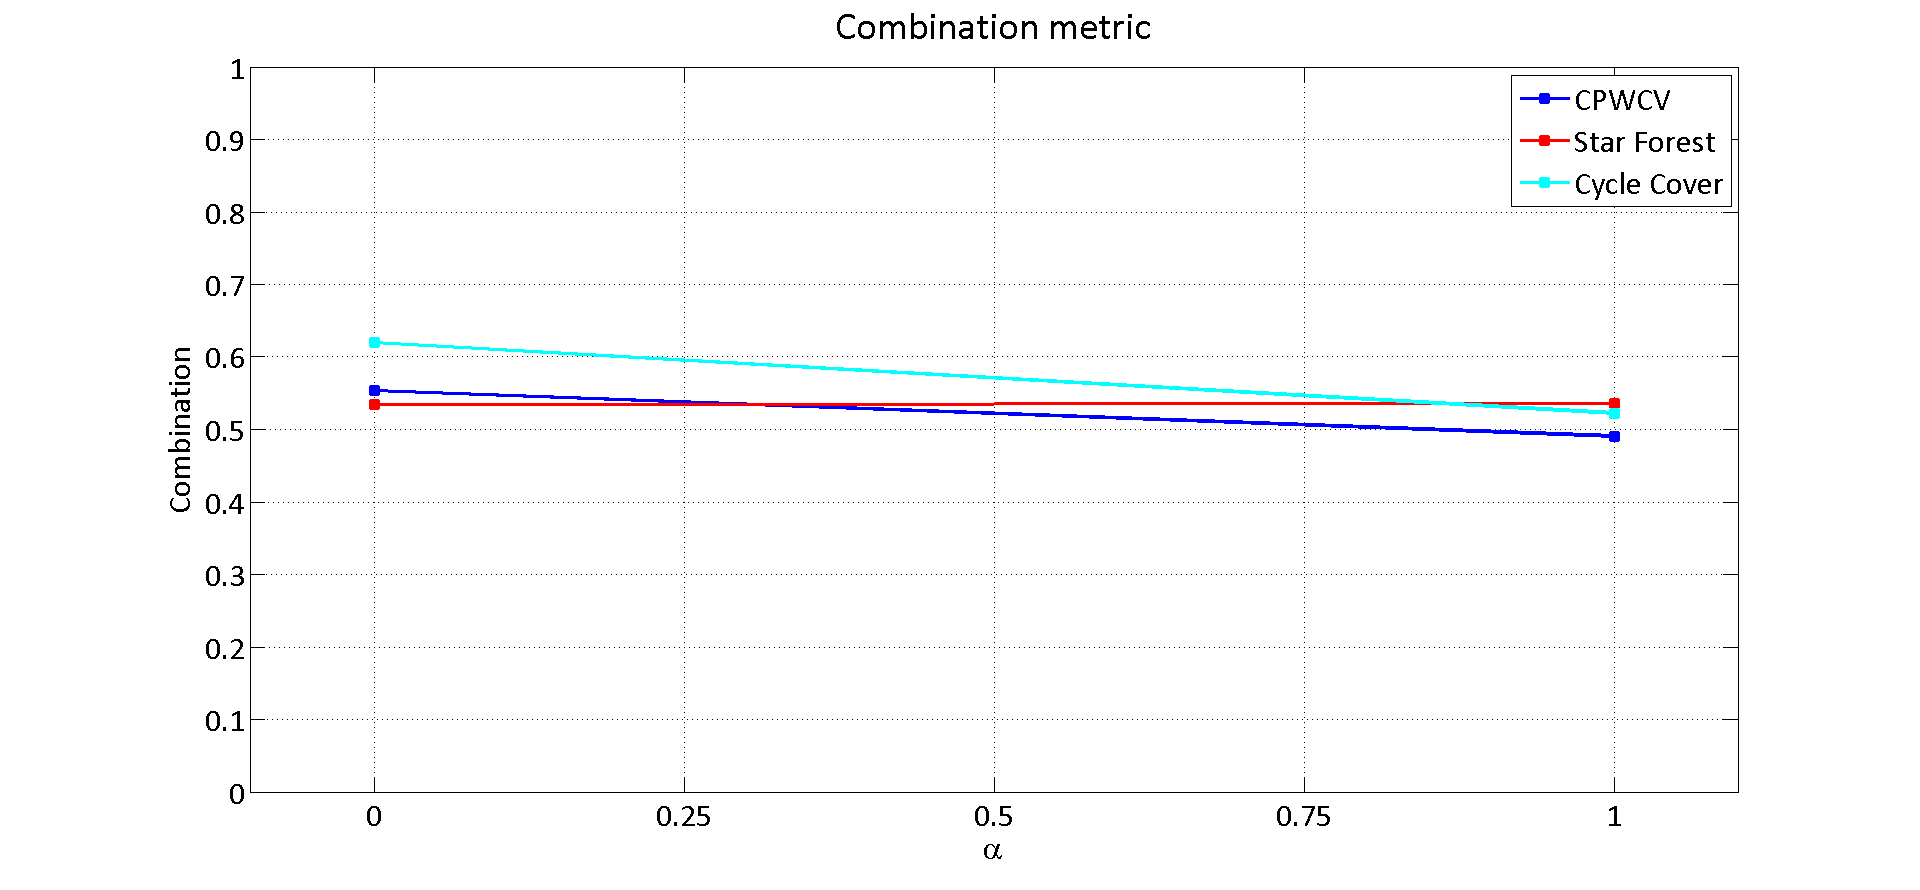
\includegraphics[scale=0.35]{img/impl_test/test_tf_jaccard/figures/combo_60.png}}
\caption{Combination metric: Term Frequency + Jaccard Similarity con 60 parole estratte.}
\label{combo_tf_jaccard_60}
\end{figure}
\begin{figure}
\centering
{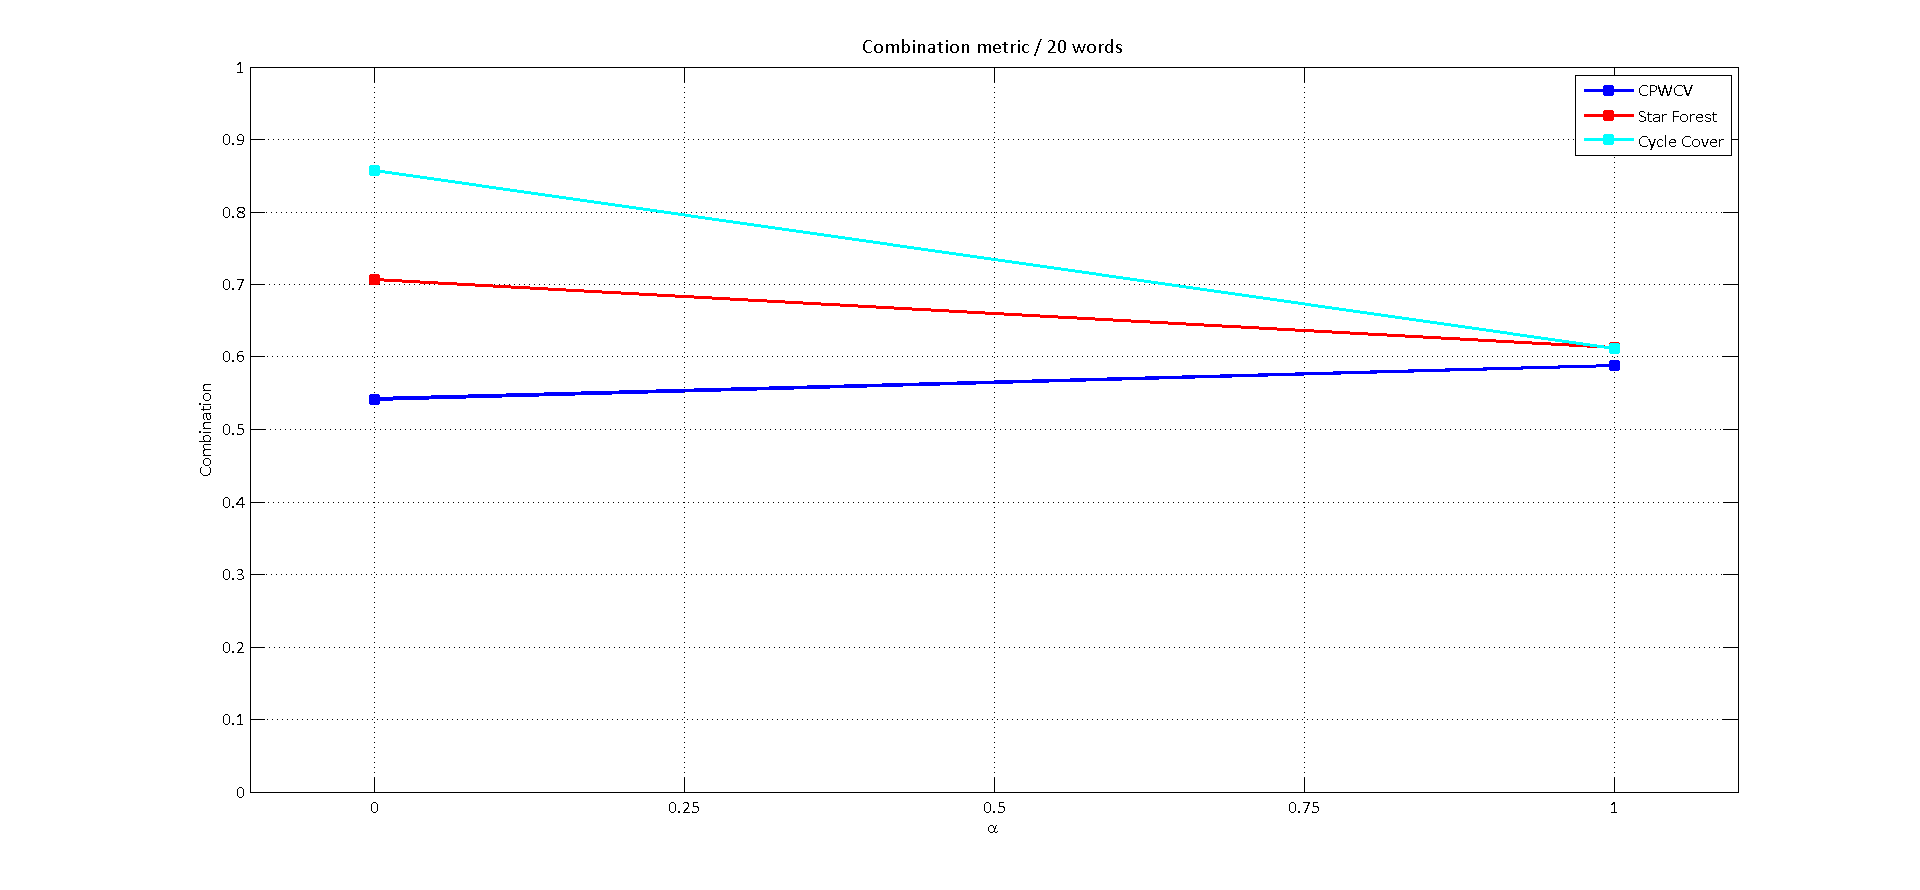
\includegraphics[scale=0.35]{img/impl_test/test_tf_cosine/figures/combo_20.png}}
\caption{Combination metric: Term Frequency + Cosine Similarity con 20 parole estratte.}
\label{combo_tf_cosine_20}
\end{figure}
\begin{figure}
\centering
{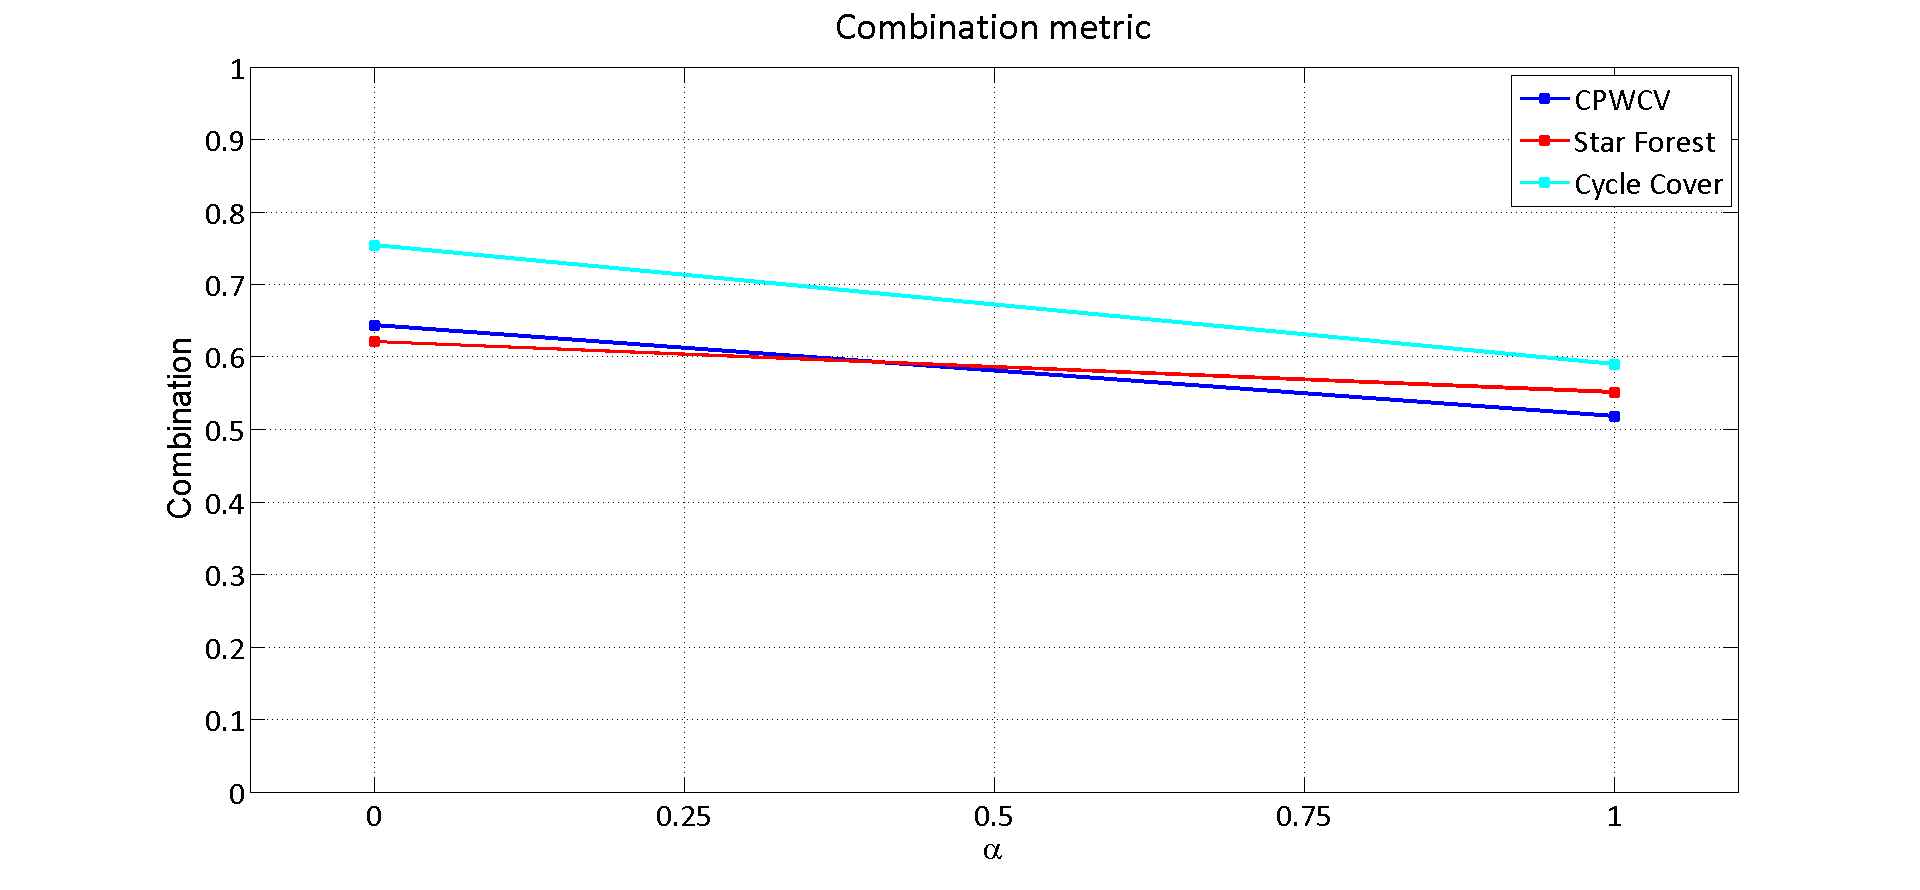
\includegraphics[scale=0.35]{img/impl_test/test_tf_cosine/figures/combo_40.png}}
\caption{Combination metric: Term Frequency + Cosine Similarity con 40 parole estratte.}
\label{sm_tf_cosine_40}
\end{figure}
\begin{figure}
\centering
{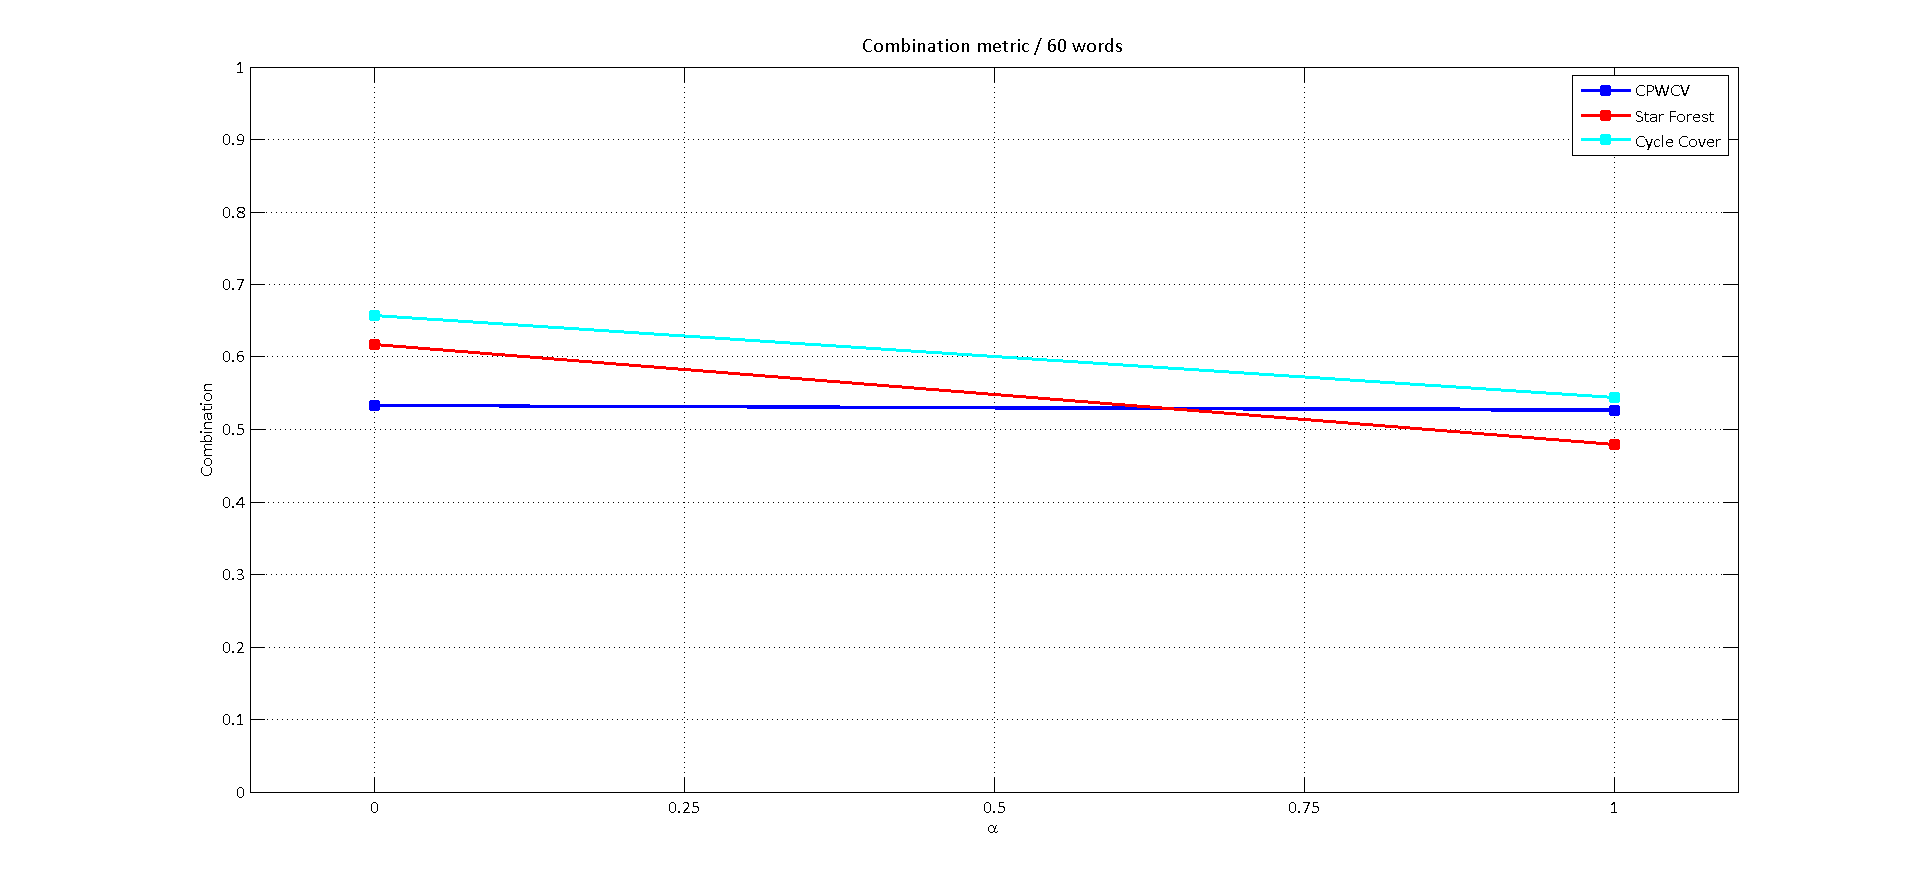
\includegraphics[scale=0.35]{img/impl_test/test_tf_cosine/figures/combo_60.png}}
\caption{Combination metric: Term Frequency + Cosine Similarity con 60 parole estratte.}
\label{sm_tf_cosine_60}
\end{figure}
\begin{figure}
\centering
{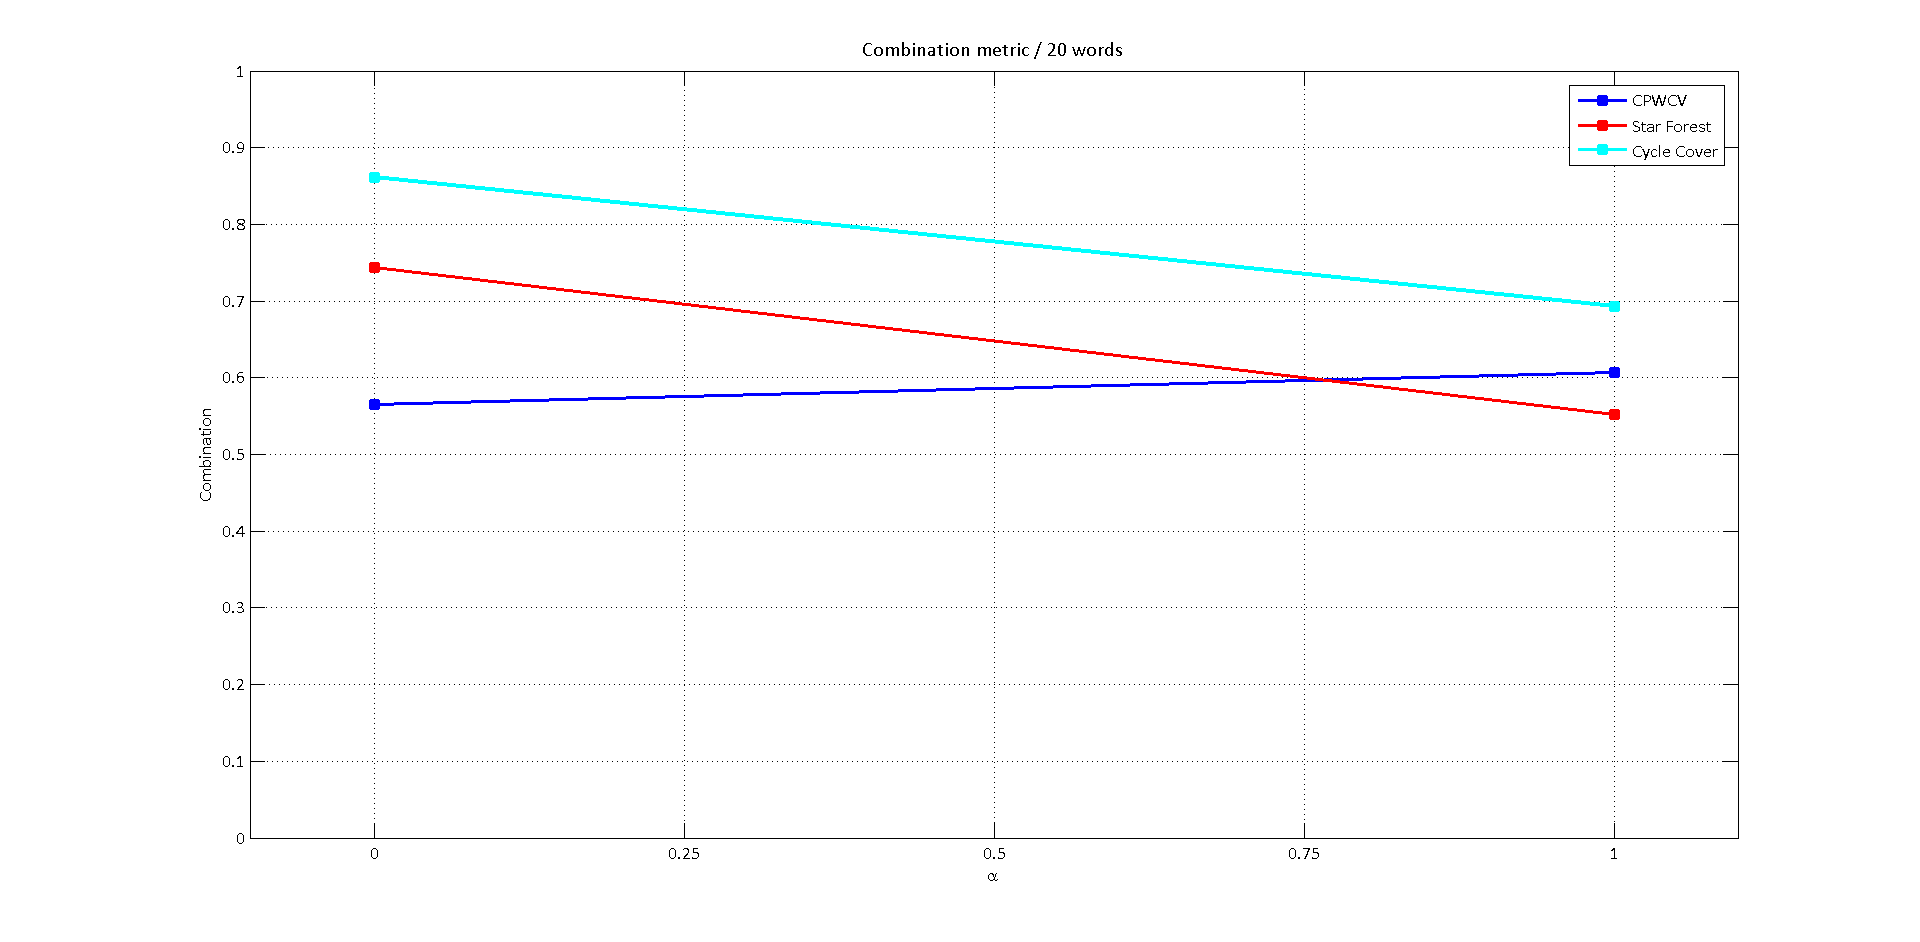
\includegraphics[scale=0.35]{img/impl_test/test_tf_extended/figures/combo_20.png}}
\caption{Combination metric: Term Frequency + Extended Jaccard Similarity con 20 parole estratte.}
\label{combo_tf_extended_20}
\end{figure}
\begin{figure}
\centering
{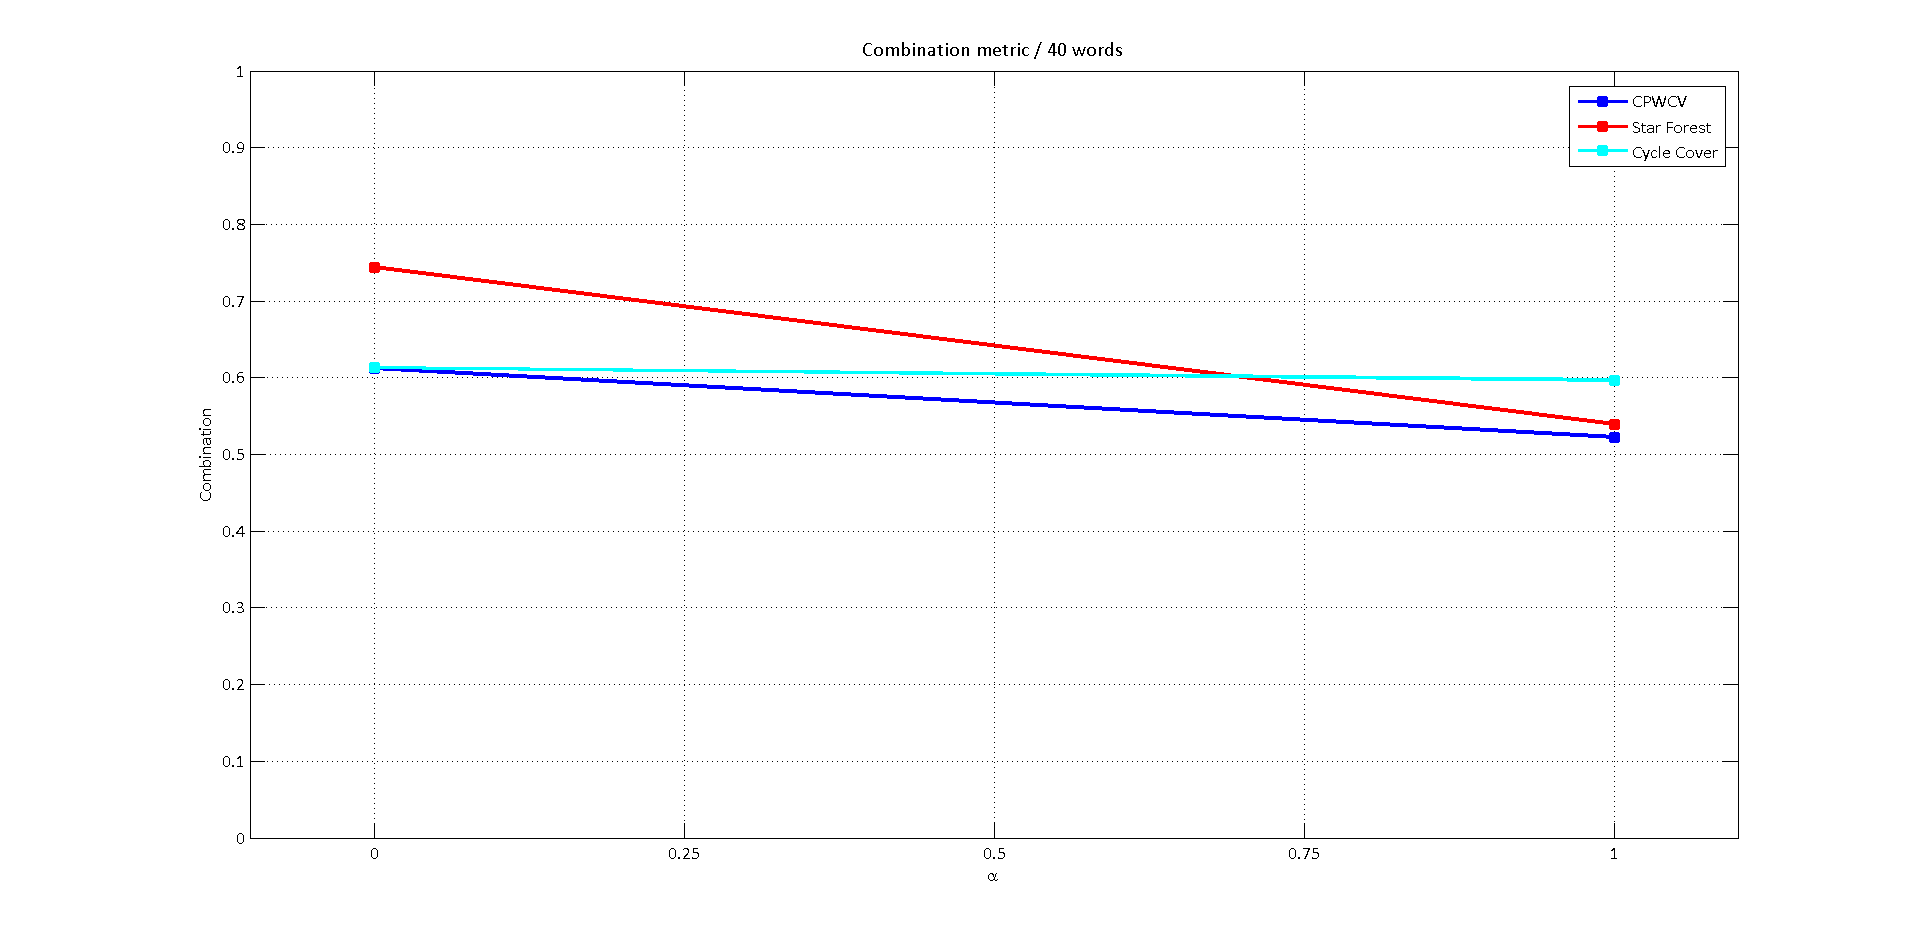
\includegraphics[scale=0.35]{img/impl_test/test_tf_extended/figures/combo_40.png}}
\caption{Combination metric: Term Frequency + Extended Jaccard Similarity con 40 parole estratte.}
\label{combo_tf_extended_40}
\end{figure}
\clearpage
\begin{figure}
\centering
{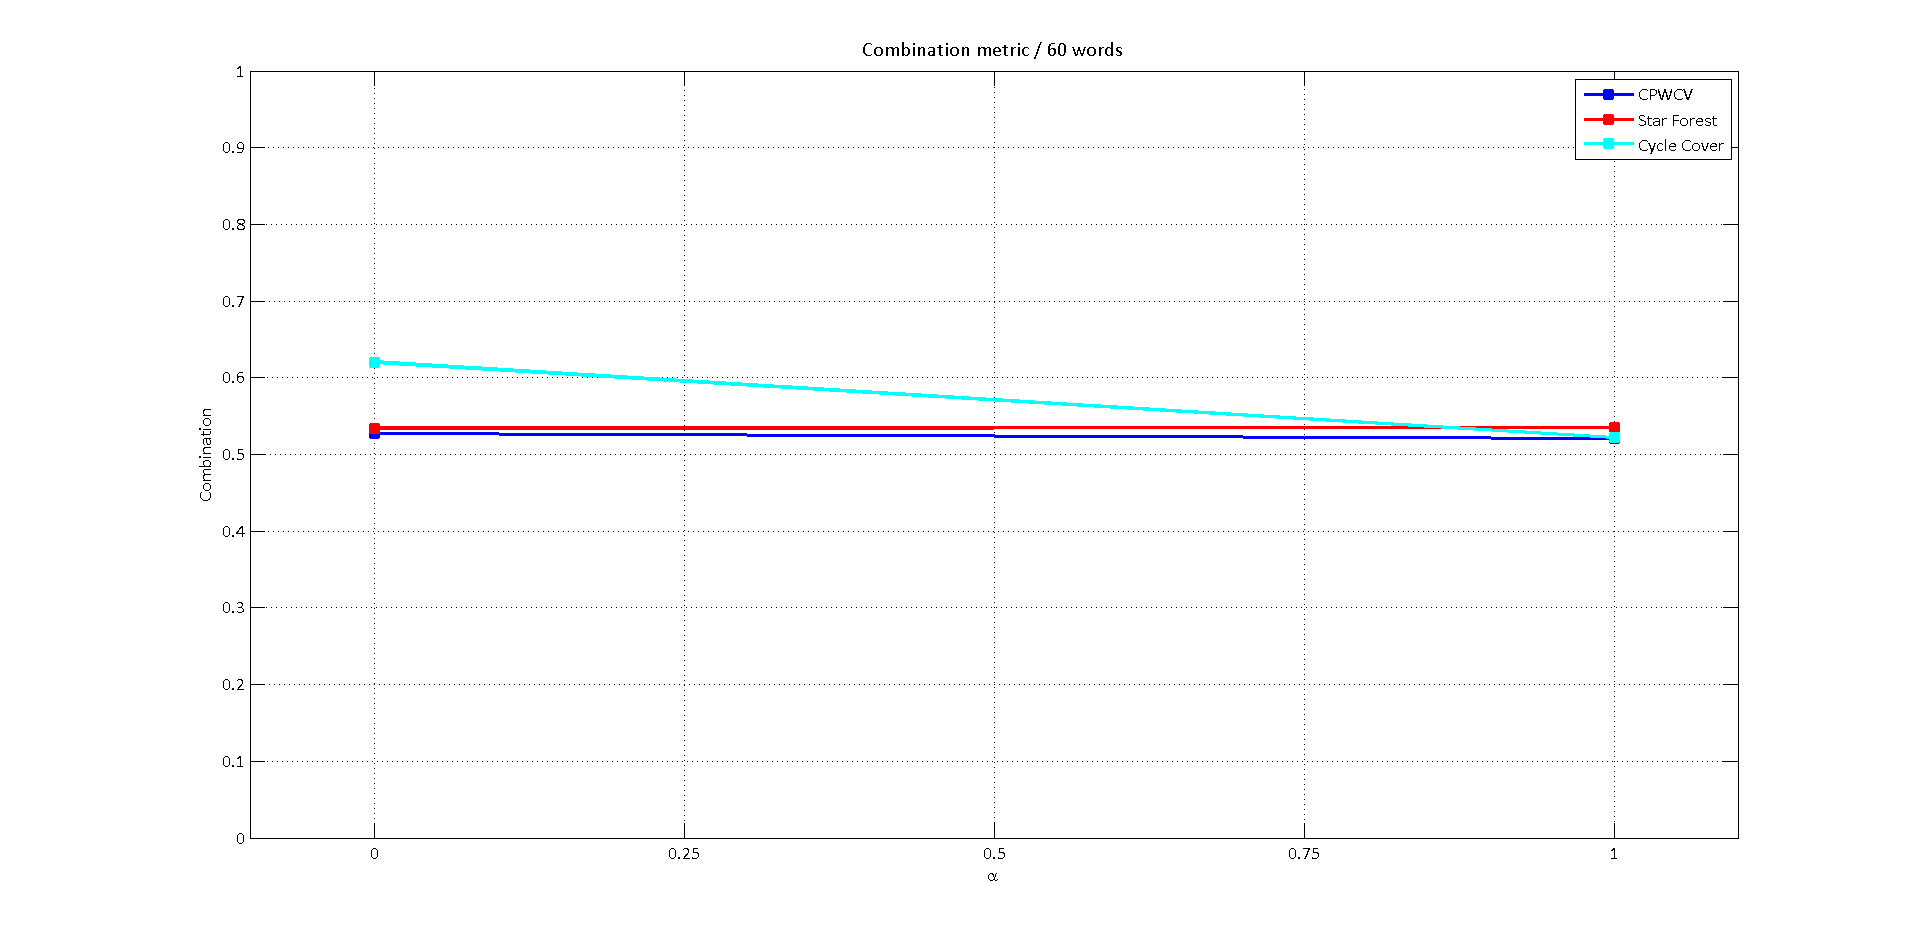
\includegraphics[scale=0.35]{img/impl_test/test_tf_extended/figures/combo_60.png}}
\caption{Combination metric: Term Frequency + Extended Jaccard Similarity con 60 parole estratte.}
\label{combo_tf_extended_60}
\end{figure}
\begin{figure}
\centering
{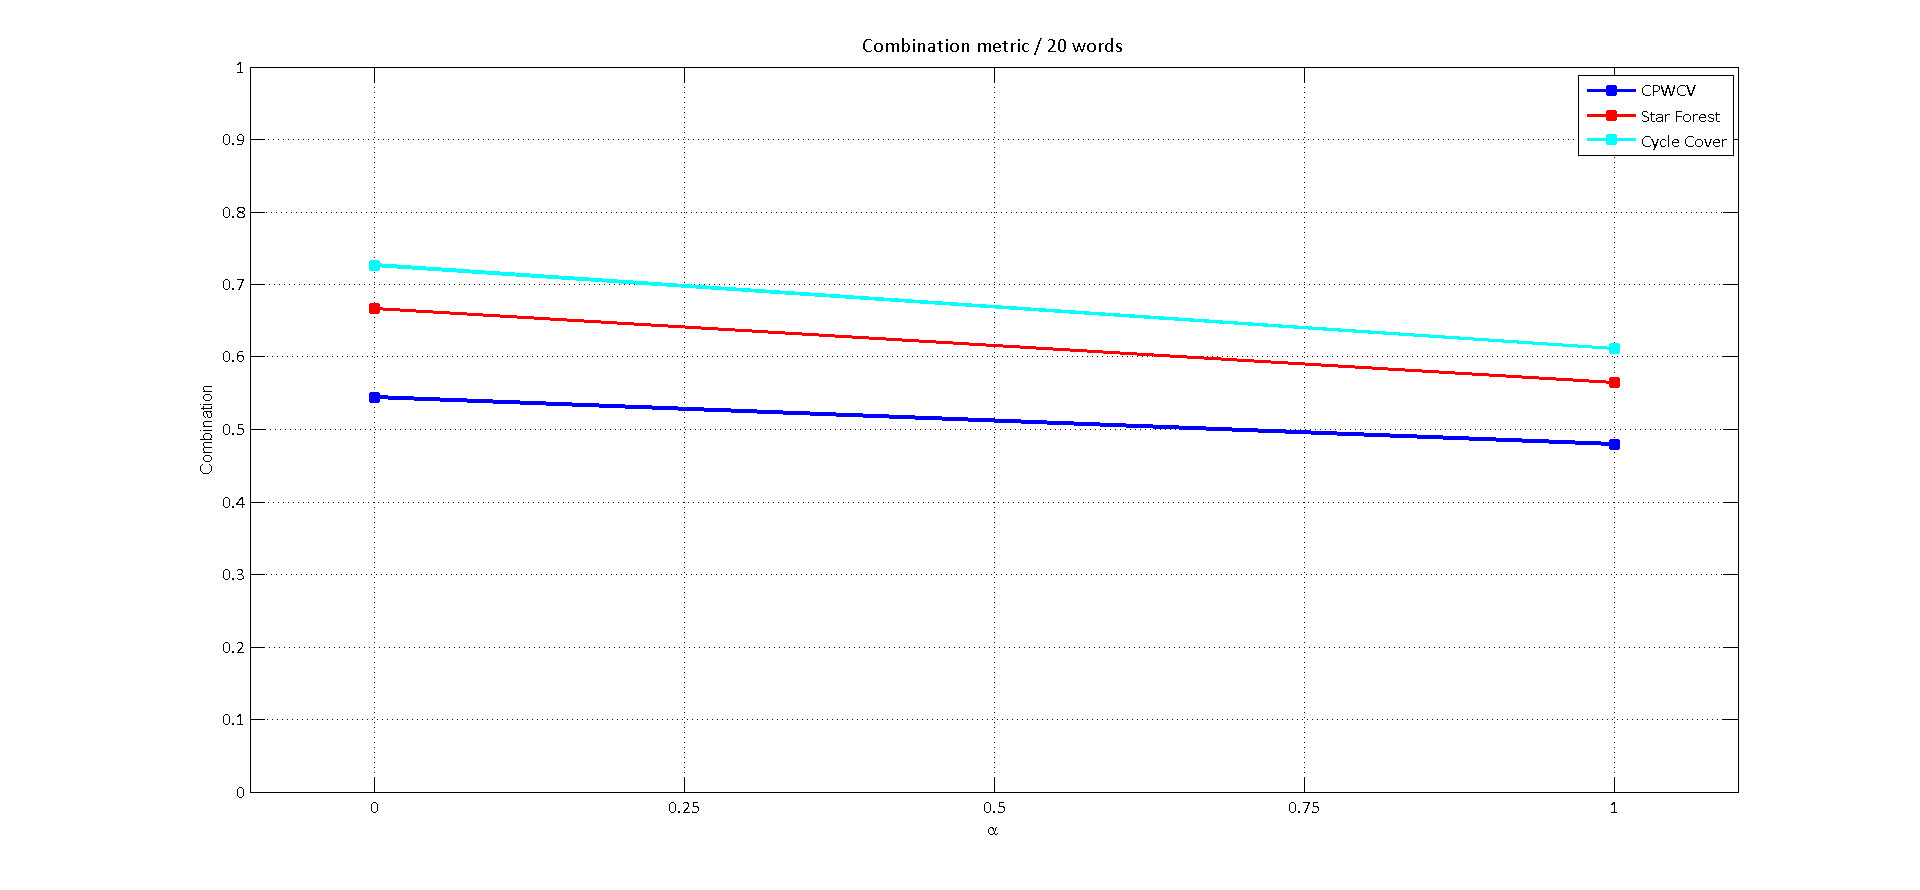
\includegraphics[scale=0.35]{img/impl_test/test_tfidf_jaccard/figures/combo_20.png}}
\caption{Combination metric: TFIDF + Jaccard Similarity con 20 parole estratte.}
\label{combo_tfidf_jaccard_20}
\end{figure}
\begin{figure}
\centering
{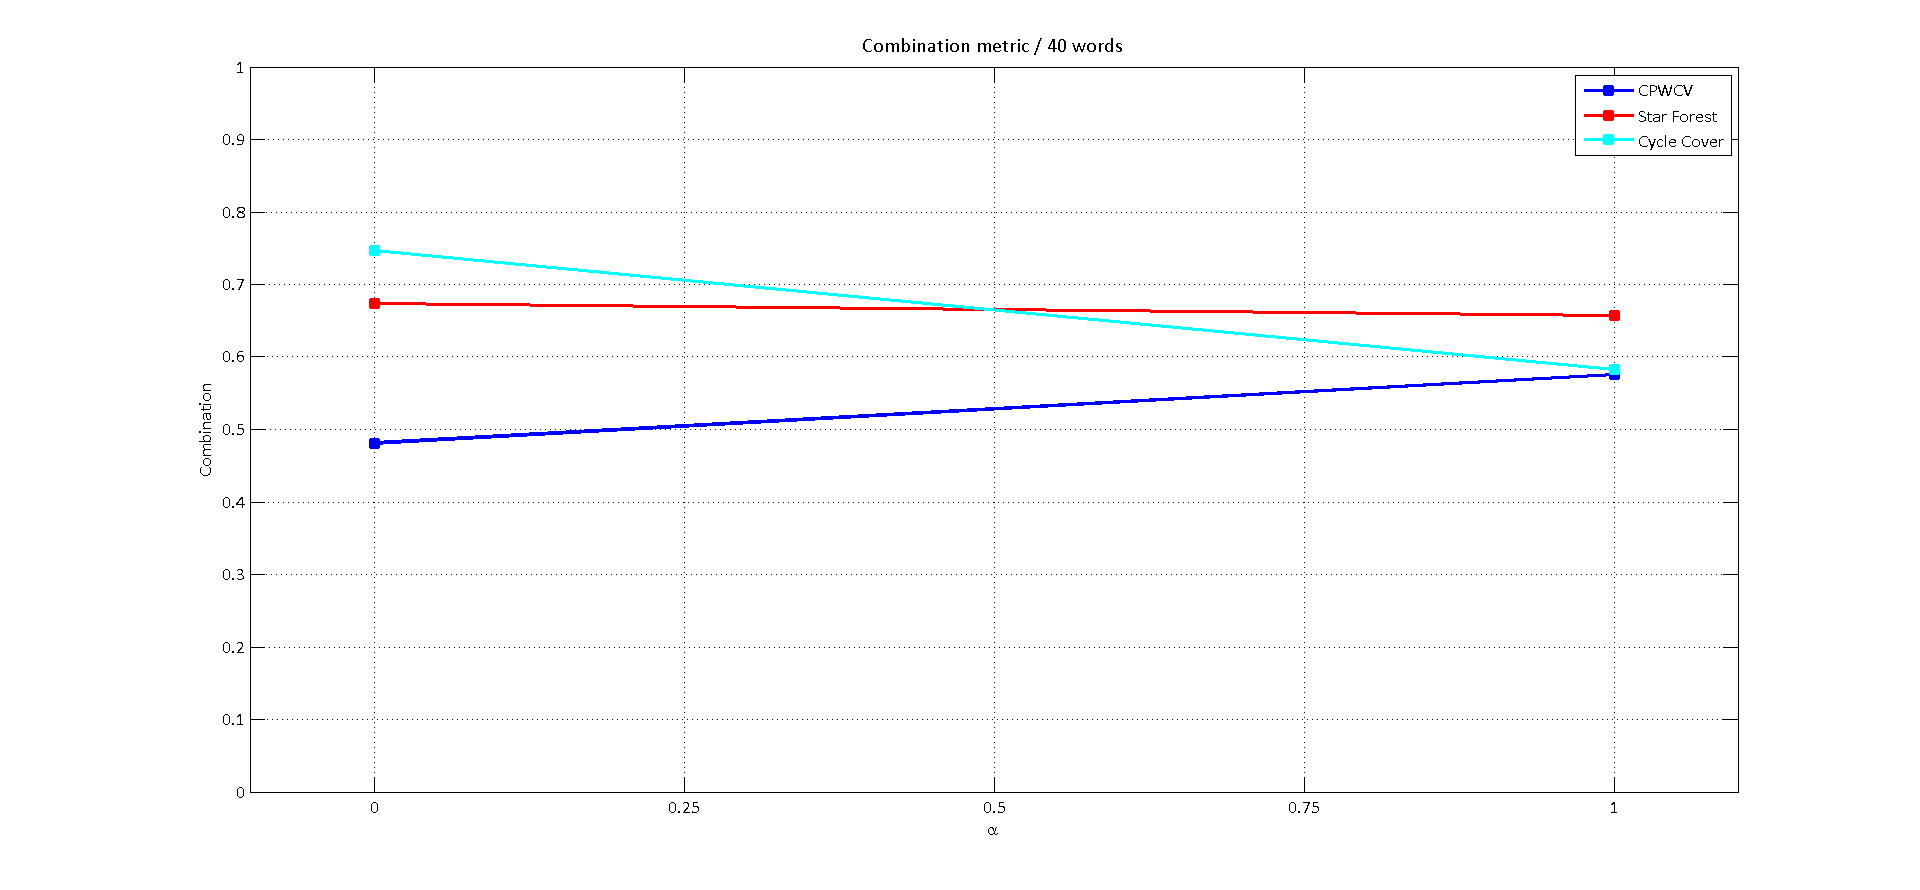
\includegraphics[scale=0.35]{img/impl_test/test_tfidf_jaccard/figures/combo_40.png}}
\caption{Combination metric: TFIDF + Jaccard Similarity con 40 parole estratte.}
\label{combo_tfidf_jaccard_40}
\end{figure}
\begin{figure}
\centering
{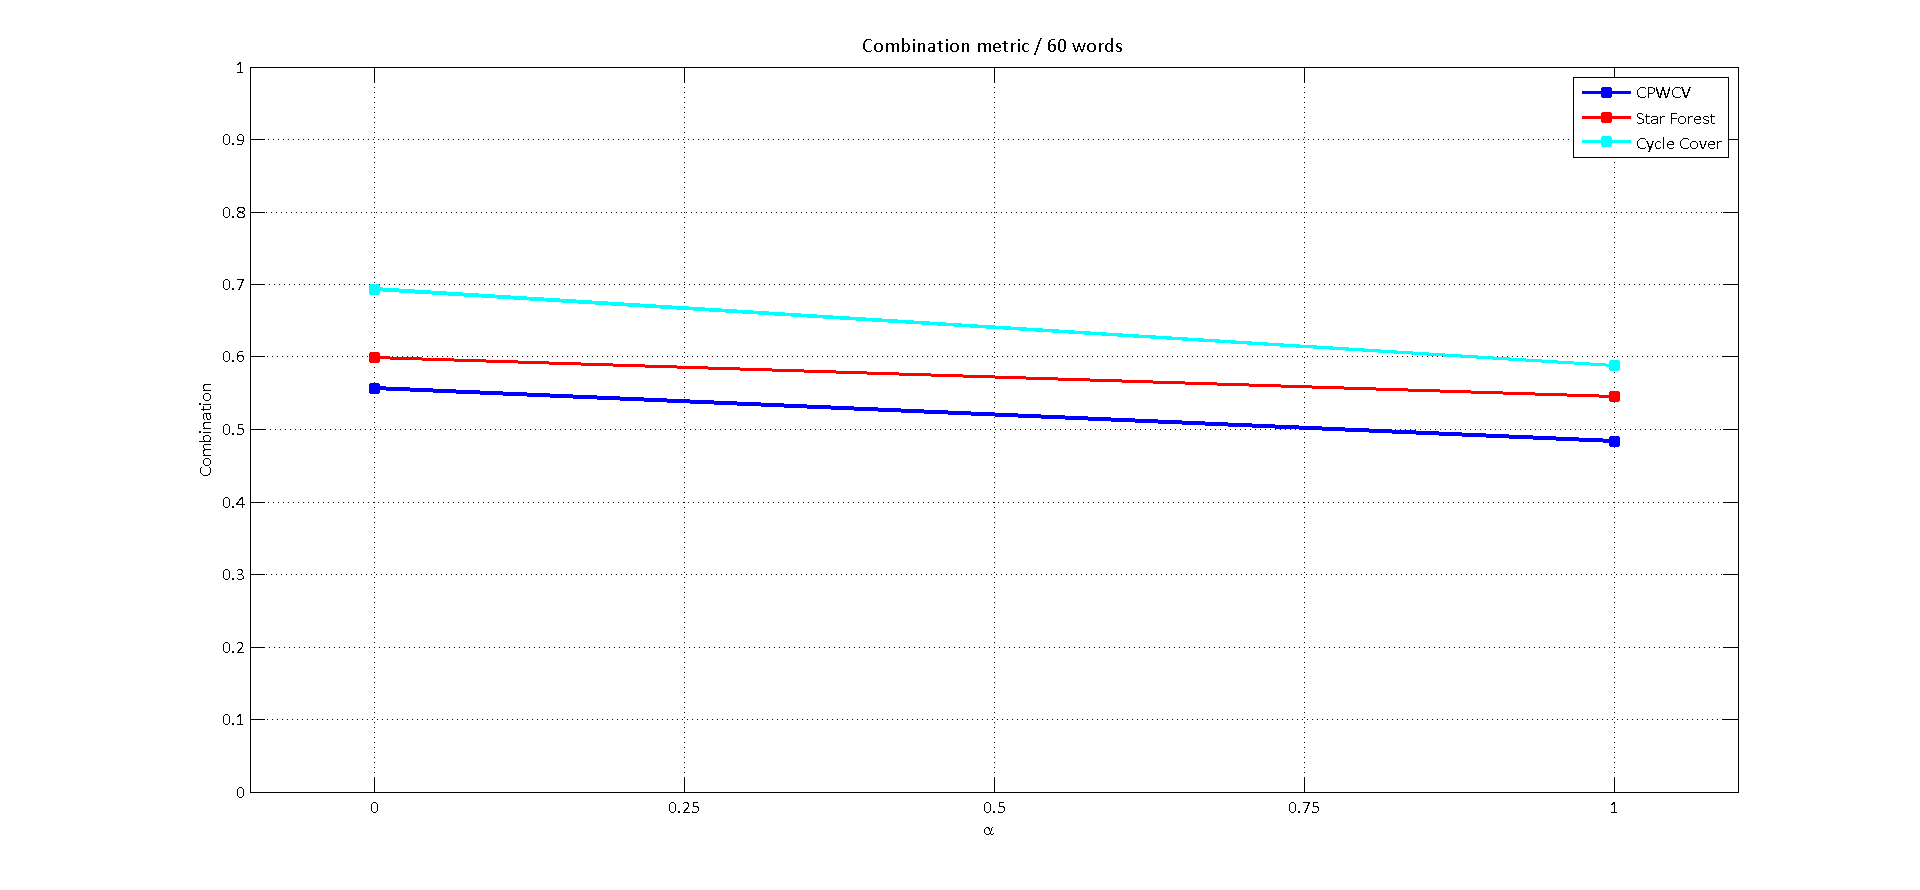
\includegraphics[scale=0.35]{img/impl_test/test_tfidf_jaccard/figures/combo_60.png}}
\caption{Combination metric: TFIDF + Jaccard Similarity con 60 parole estratte.}
\label{combo_tfidf_jaccard_60}
\end{figure}
\begin{figure}
\centering
{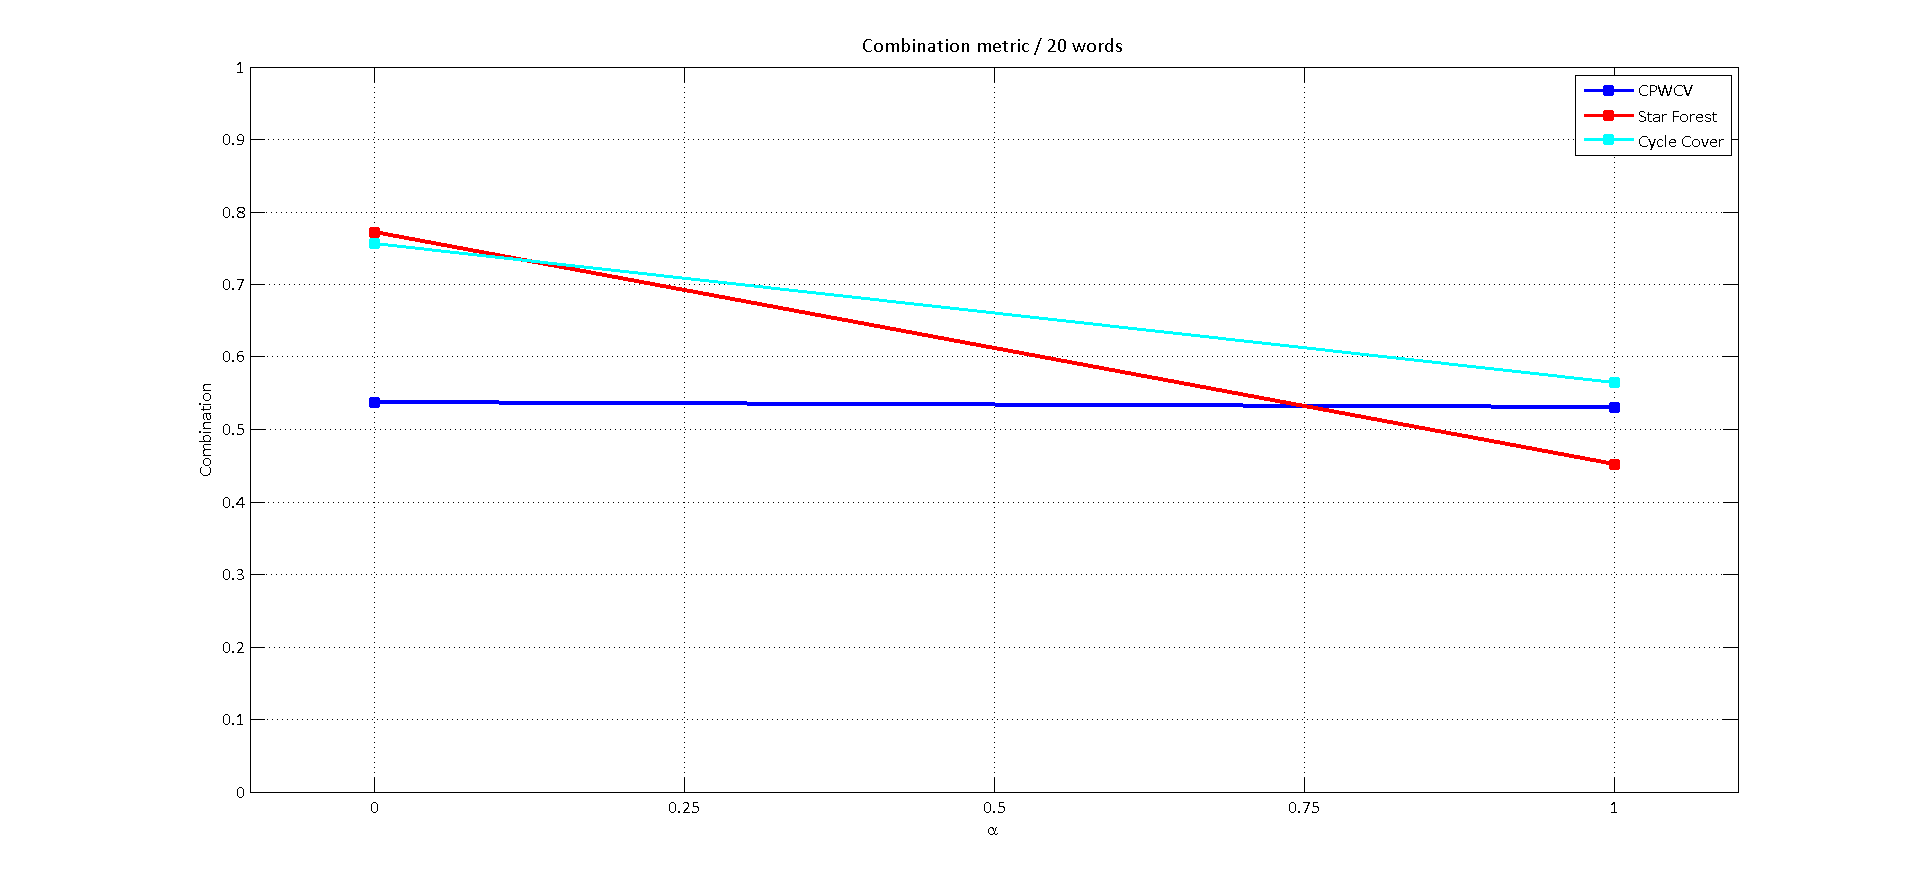
\includegraphics[scale=0.35]{img/impl_test/test_tfidf_cosine/figures/combo_20.png}}
\caption{Combination metric: TFIDF + Cosine Similarity con 20 parole estratte.}
\label{combo_tfidf_cosine_20}
\end{figure}
\begin{figure}
\centering
{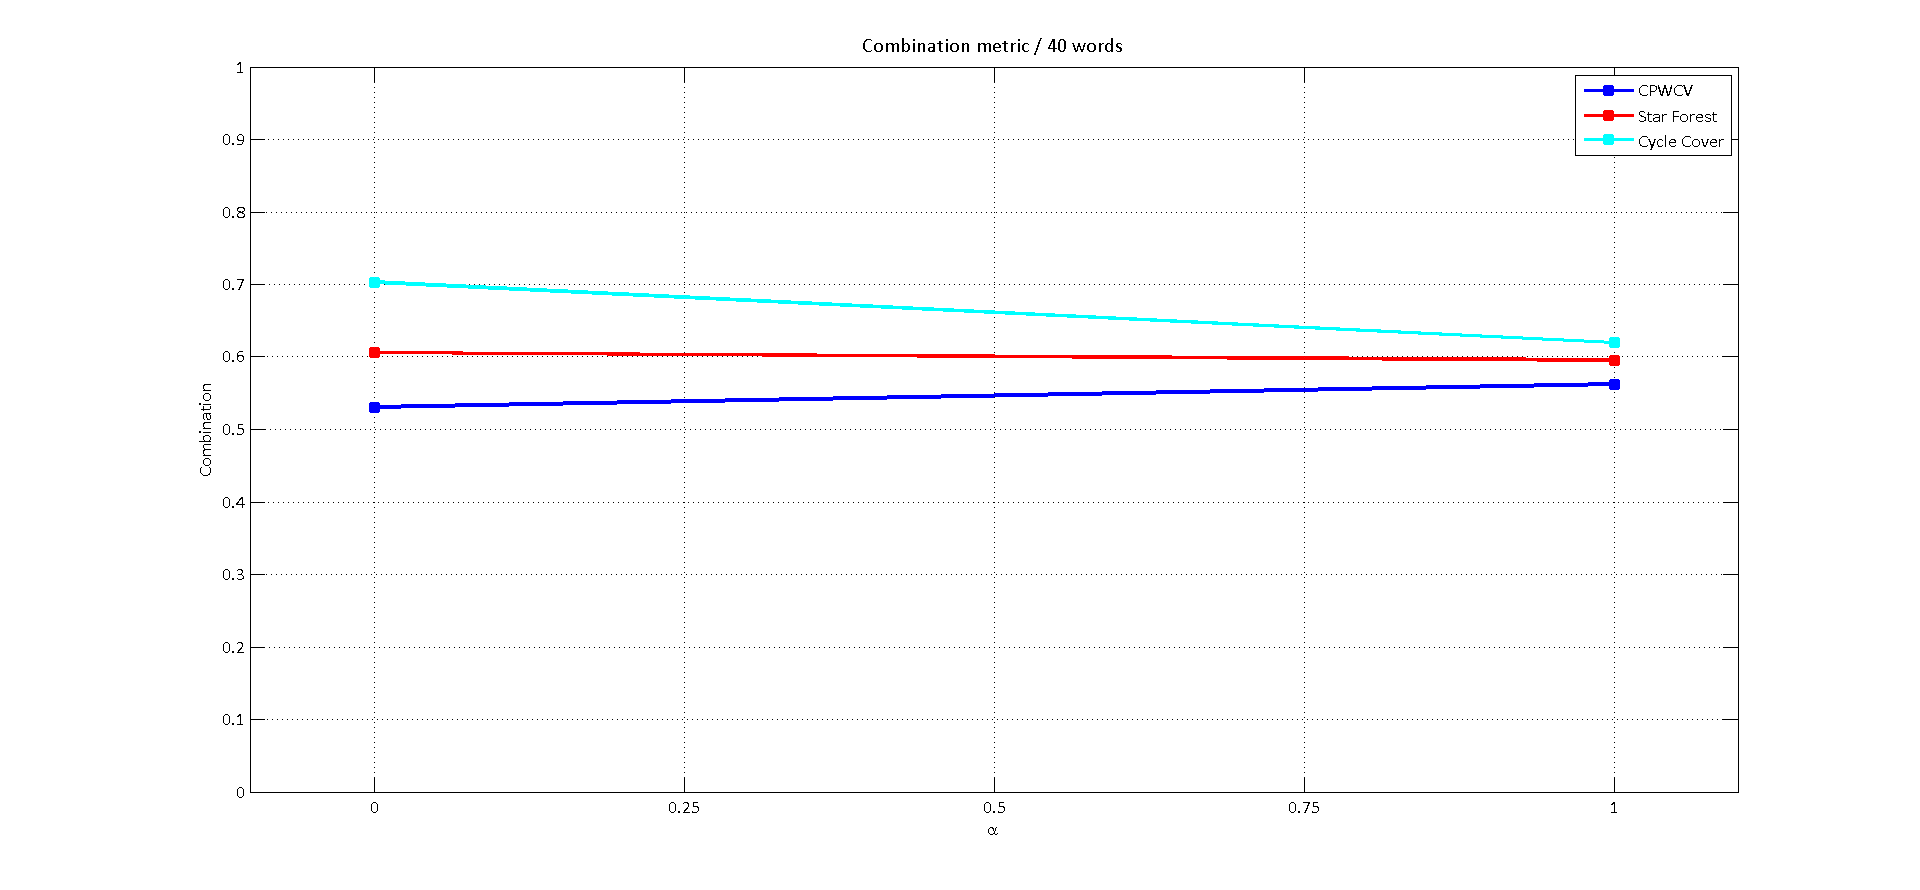
\includegraphics[scale=0.35]{img/impl_test/test_tfidf_cosine/figures/combo_40.png}}
\caption{Combination metric: TFIDF + Cosine Similarity con 40 parole estratte.}
\label{combo_tfidf_cosine_40}
\end{figure}
\begin{figure}
\centering
{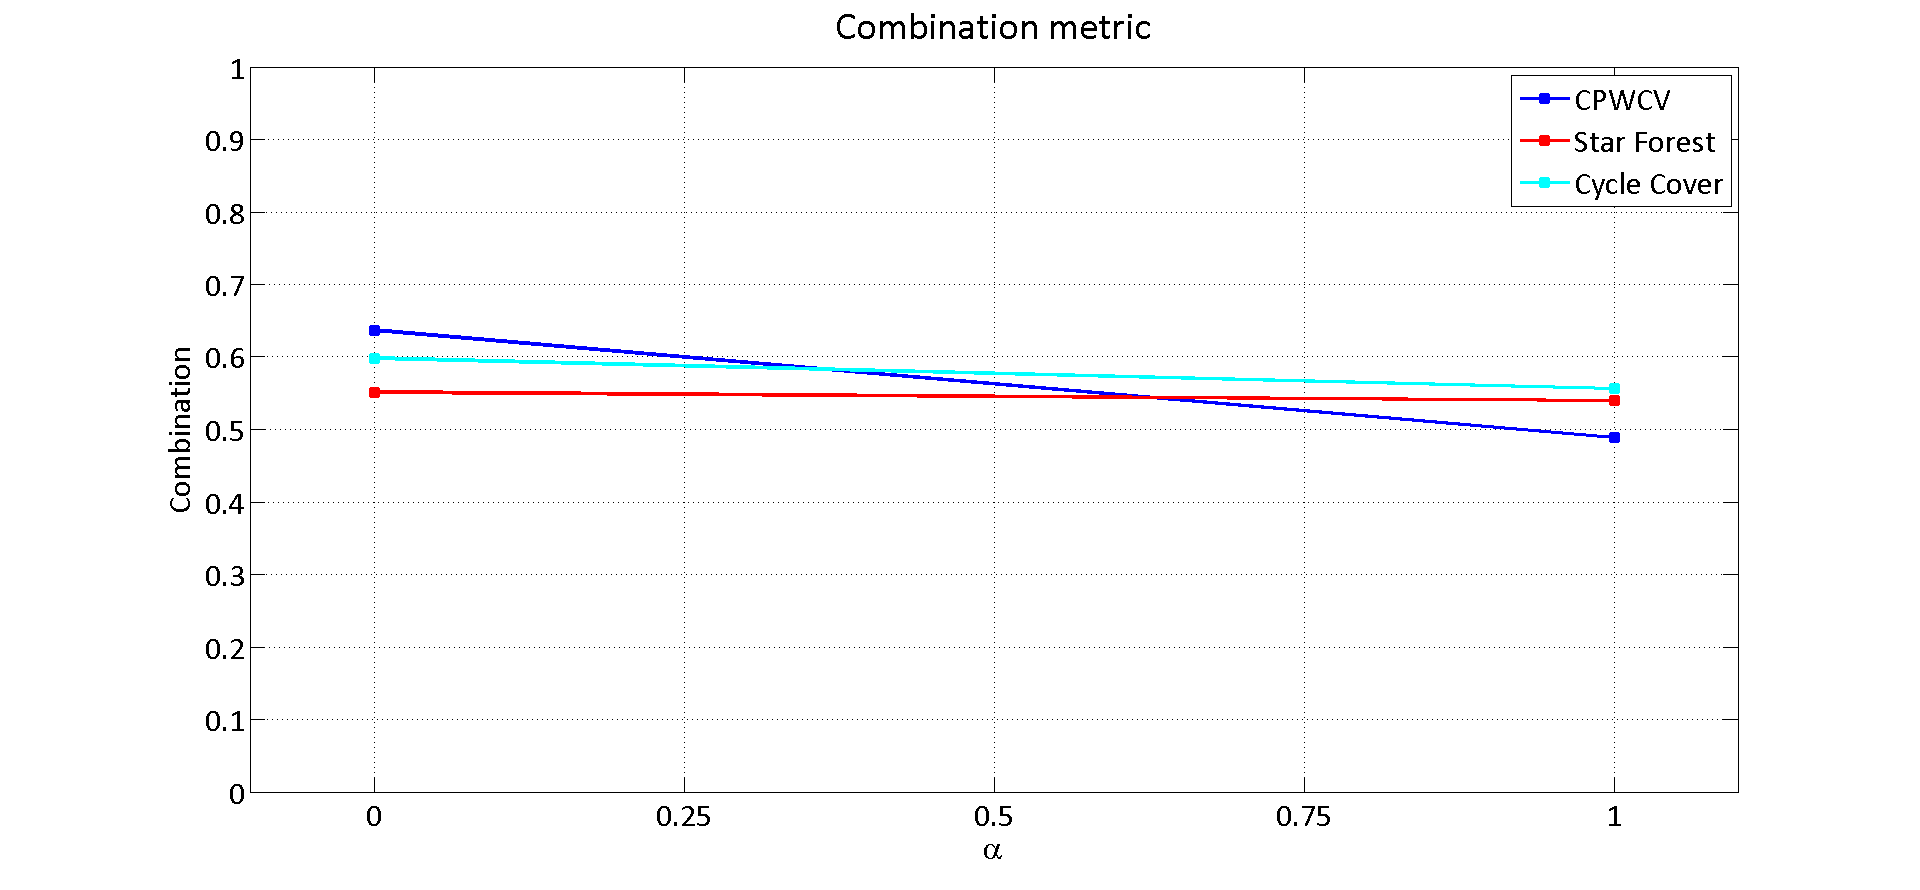
\includegraphics[scale=0.35]{img/impl_test/test_tfidf_cosine/figures/combo_60.png}}
\caption{Combination metric: TFIDF + Cosine Similarity con 60 parole estratte.}
\label{combo_tfidf_cosine_60}
\end{figure}
\begin{figure}
\centering
{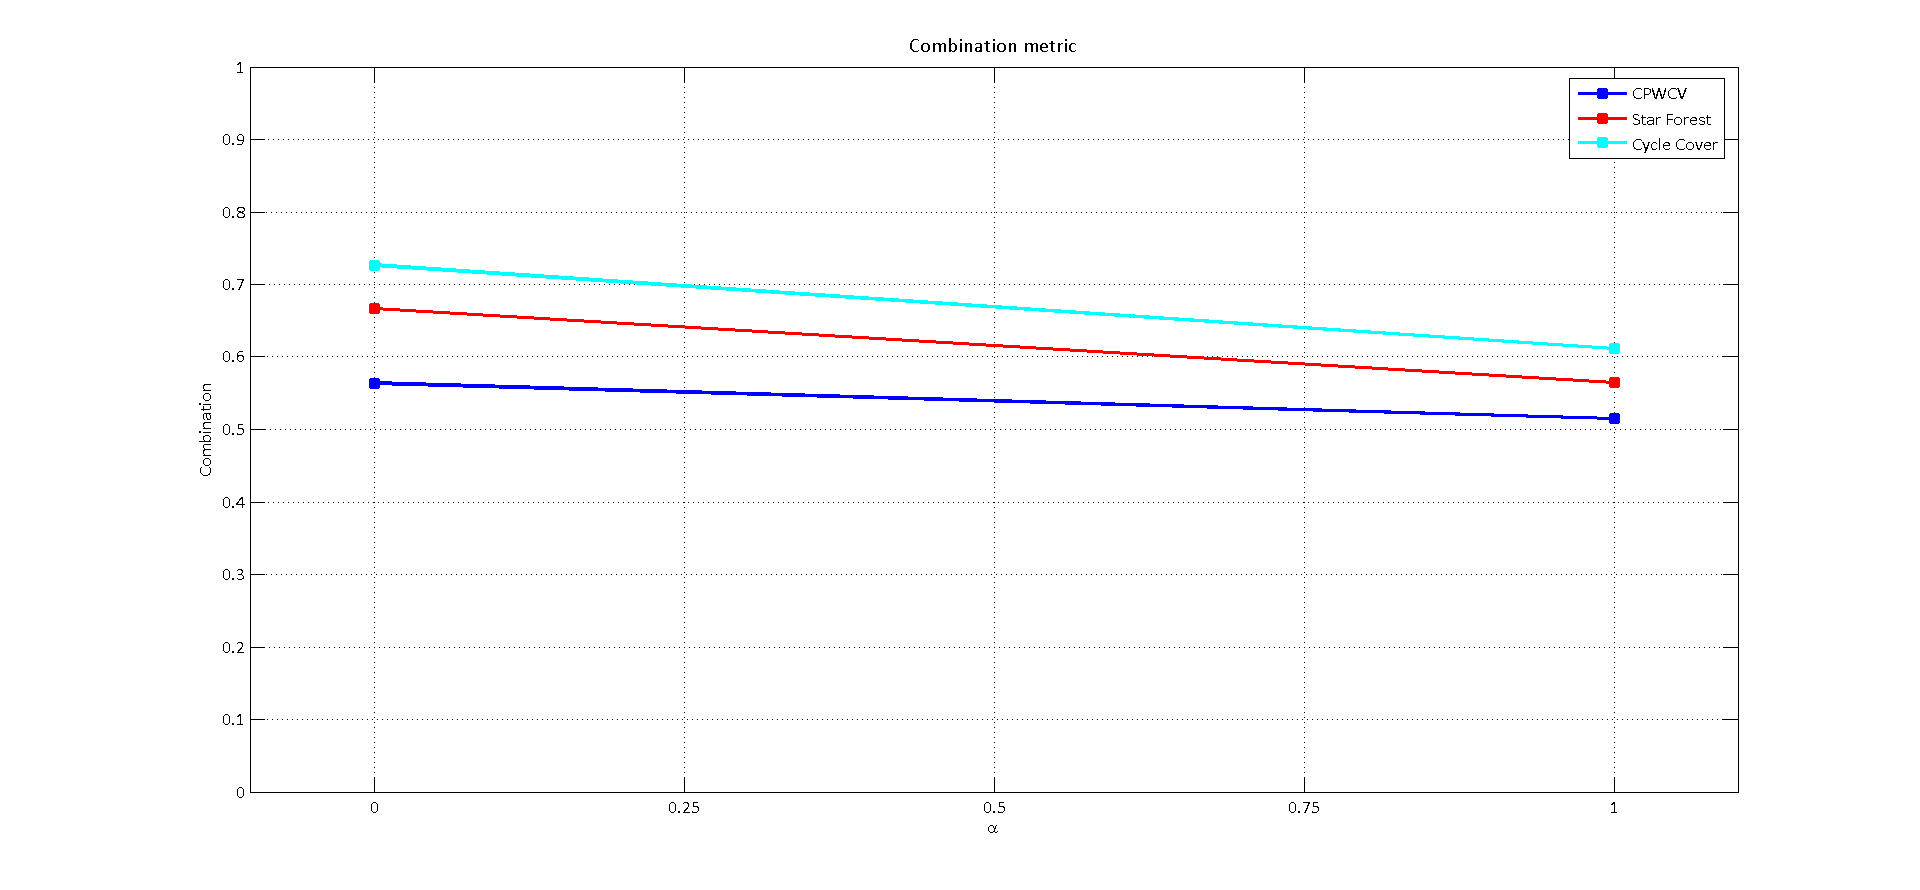
\includegraphics[scale=0.35]{img/impl_test/test_tfidf_extended/figures/combo_20.png}}
\caption{Combination metric: TFIDF + Extended Jaccard Similarity con 20 parole estratte.}
\label{combo_tfidf_extended_20}
\end{figure}
\begin{figure}
\centering
{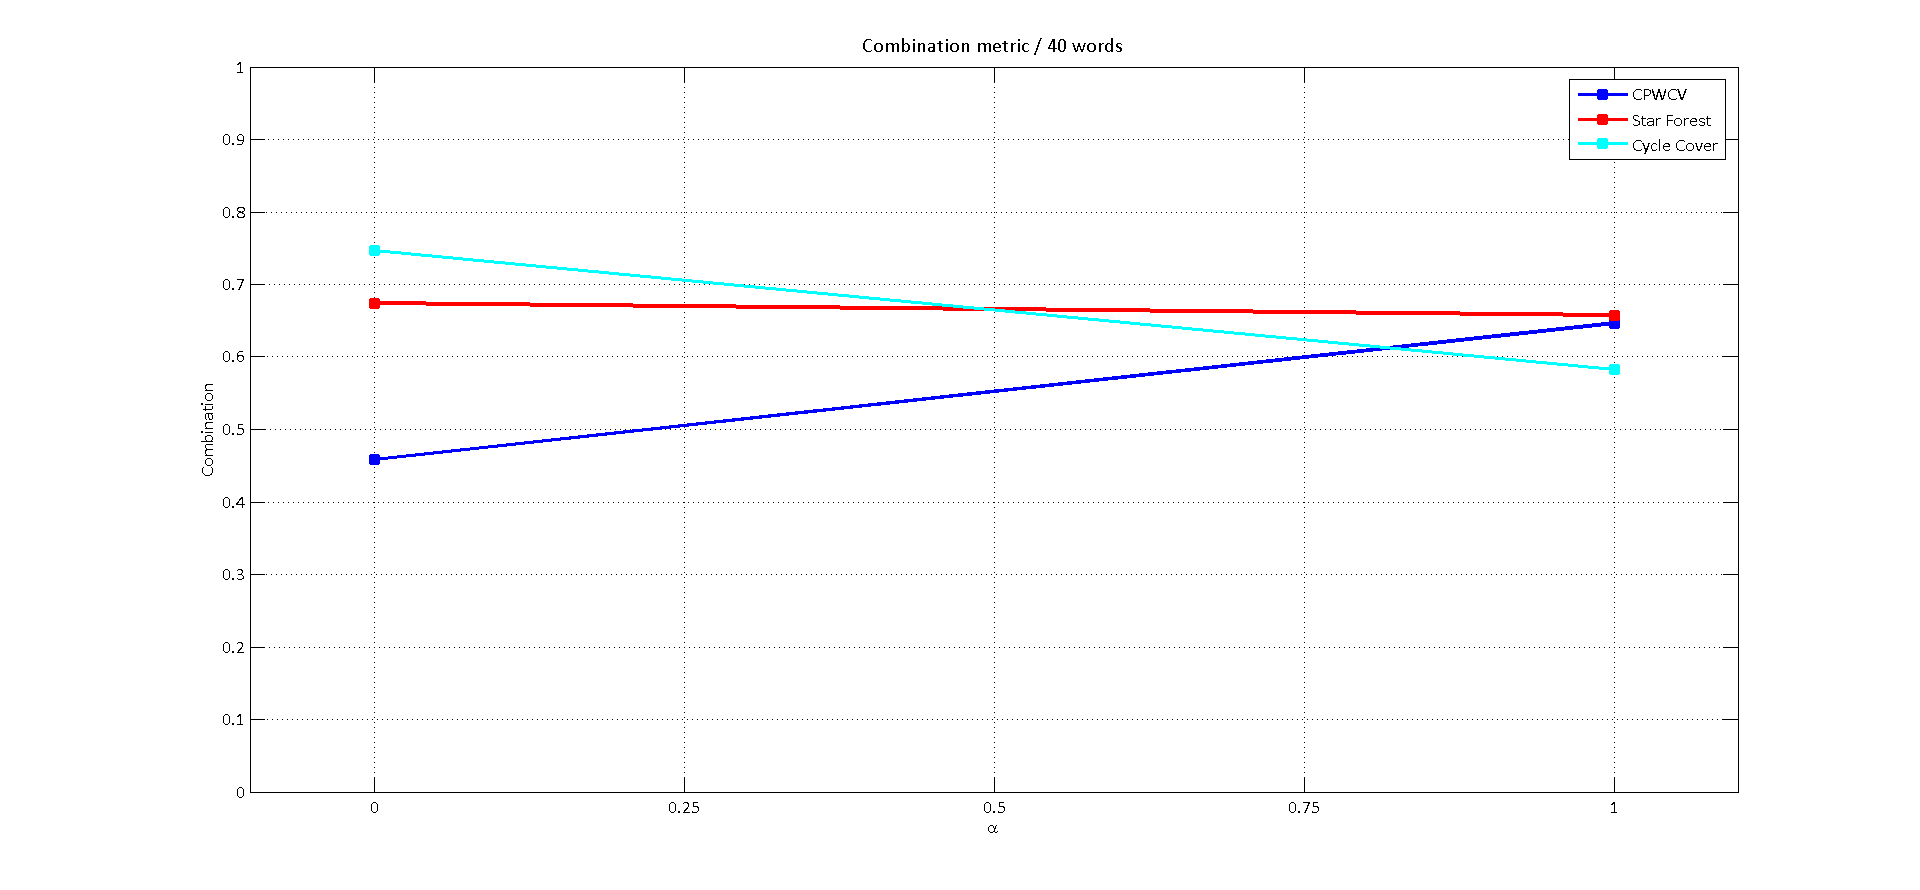
\includegraphics[scale=0.35]{img/impl_test/test_tfidf_extended/figures/combo_40.png}}
\caption{Combination metric: TFIDF + Extended Jaccard Similarity con 40 parole estratte.}
\label{combo_tfidf_extended_40}
\end{figure}
\clearpage
\begin{figure}
\centering
{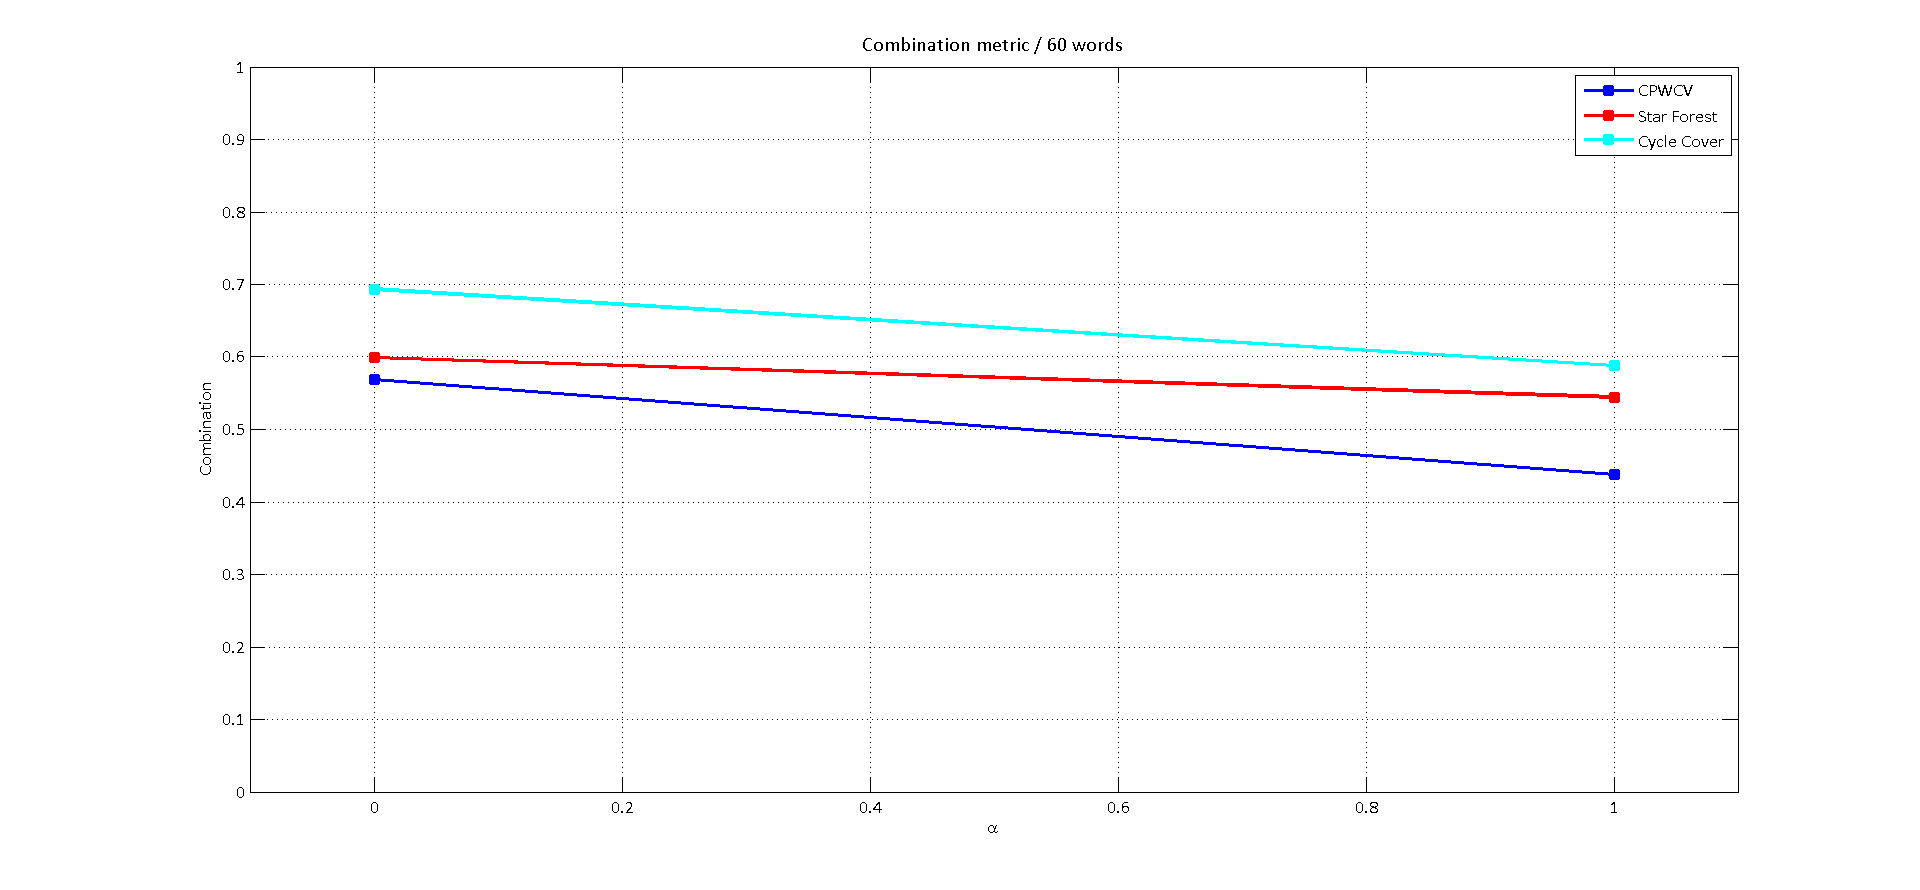
\includegraphics[scale=0.35]{img/impl_test/test_tfidf_extended/figures/combo_60.png}}
\caption{Combination metric: TFIDF + Extended Jaccard Similarity con 60 parole estratte.}
\label{combo_tfidf_extended_60}
\end{figure}
\begin{figure}
\centering
{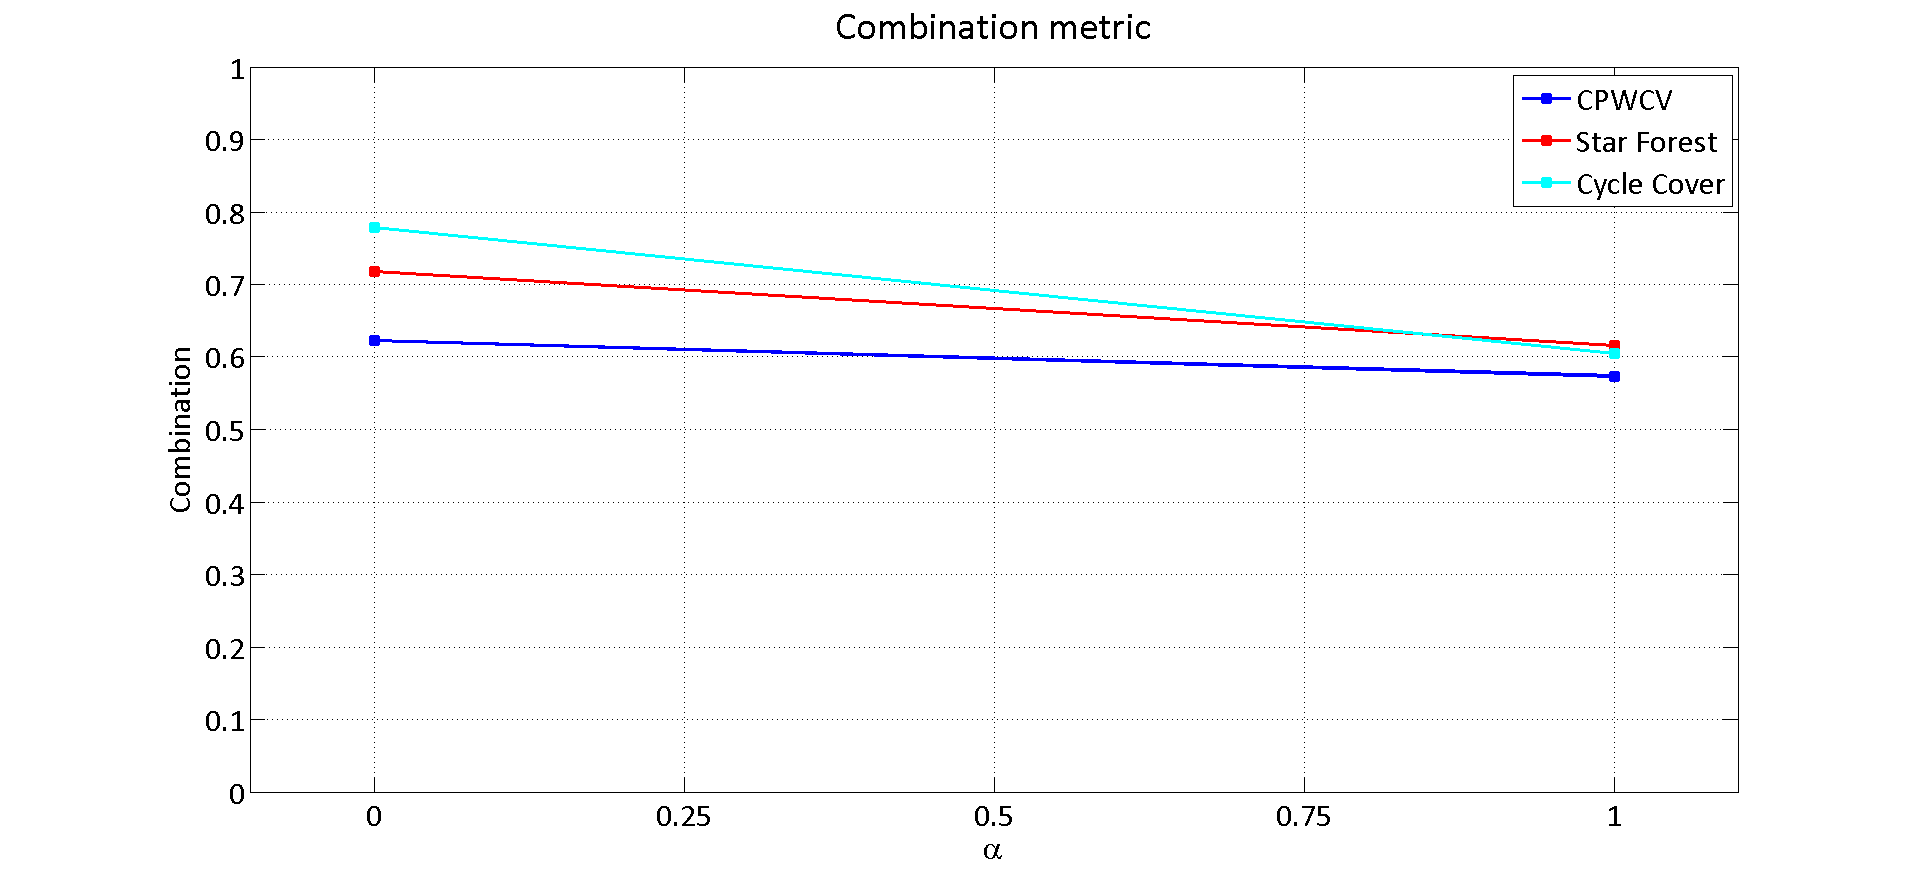
\includegraphics[scale=0.35]{img/impl_test/test_lexrank_jaccard/figures/combo_20.png}}
\caption{Combination metric: LexRank + Jaccard Similarity con 20 parole estratte.}
\label{combo_lexrank_jaccard_20}
\end{figure}
\begin{figure}
\centering
{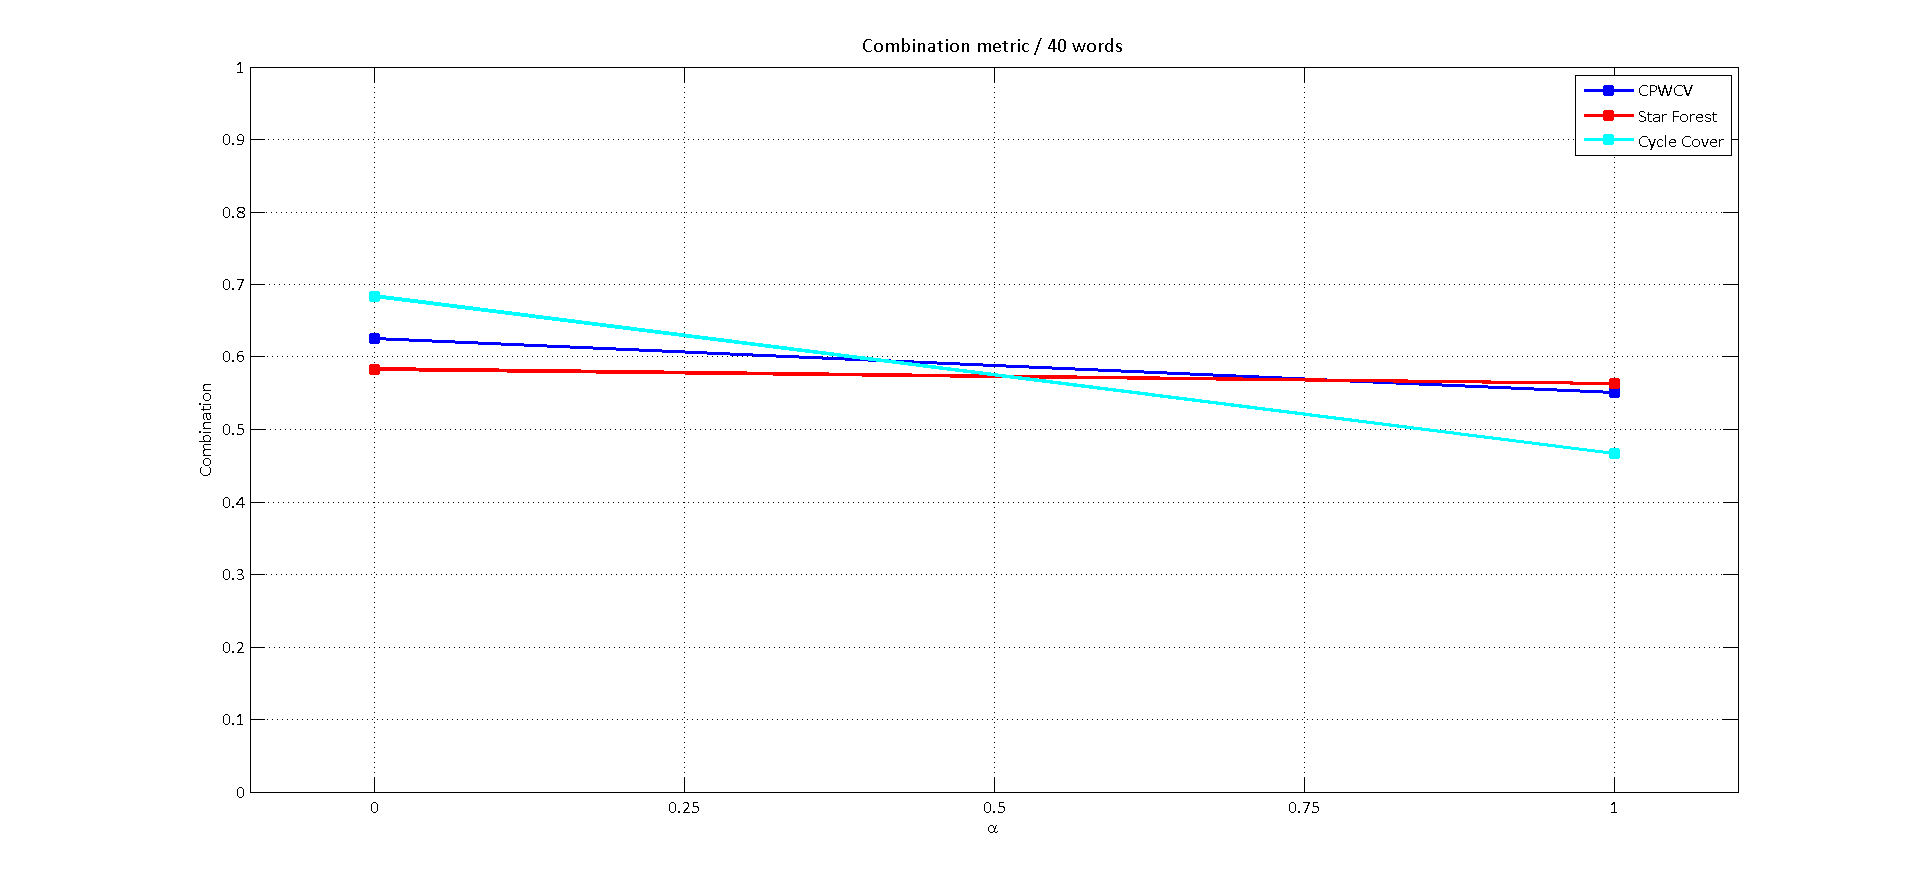
\includegraphics[scale=0.35]{img/impl_test/test_lexrank_jaccard/figures/combo_40.png}}
\caption{Combination metric: LexRank + Jaccard Similarity con 40 parole estratte.}
\label{combo_lexrank_jaccard_40}
\end{figure}
\begin{figure}
\centering
{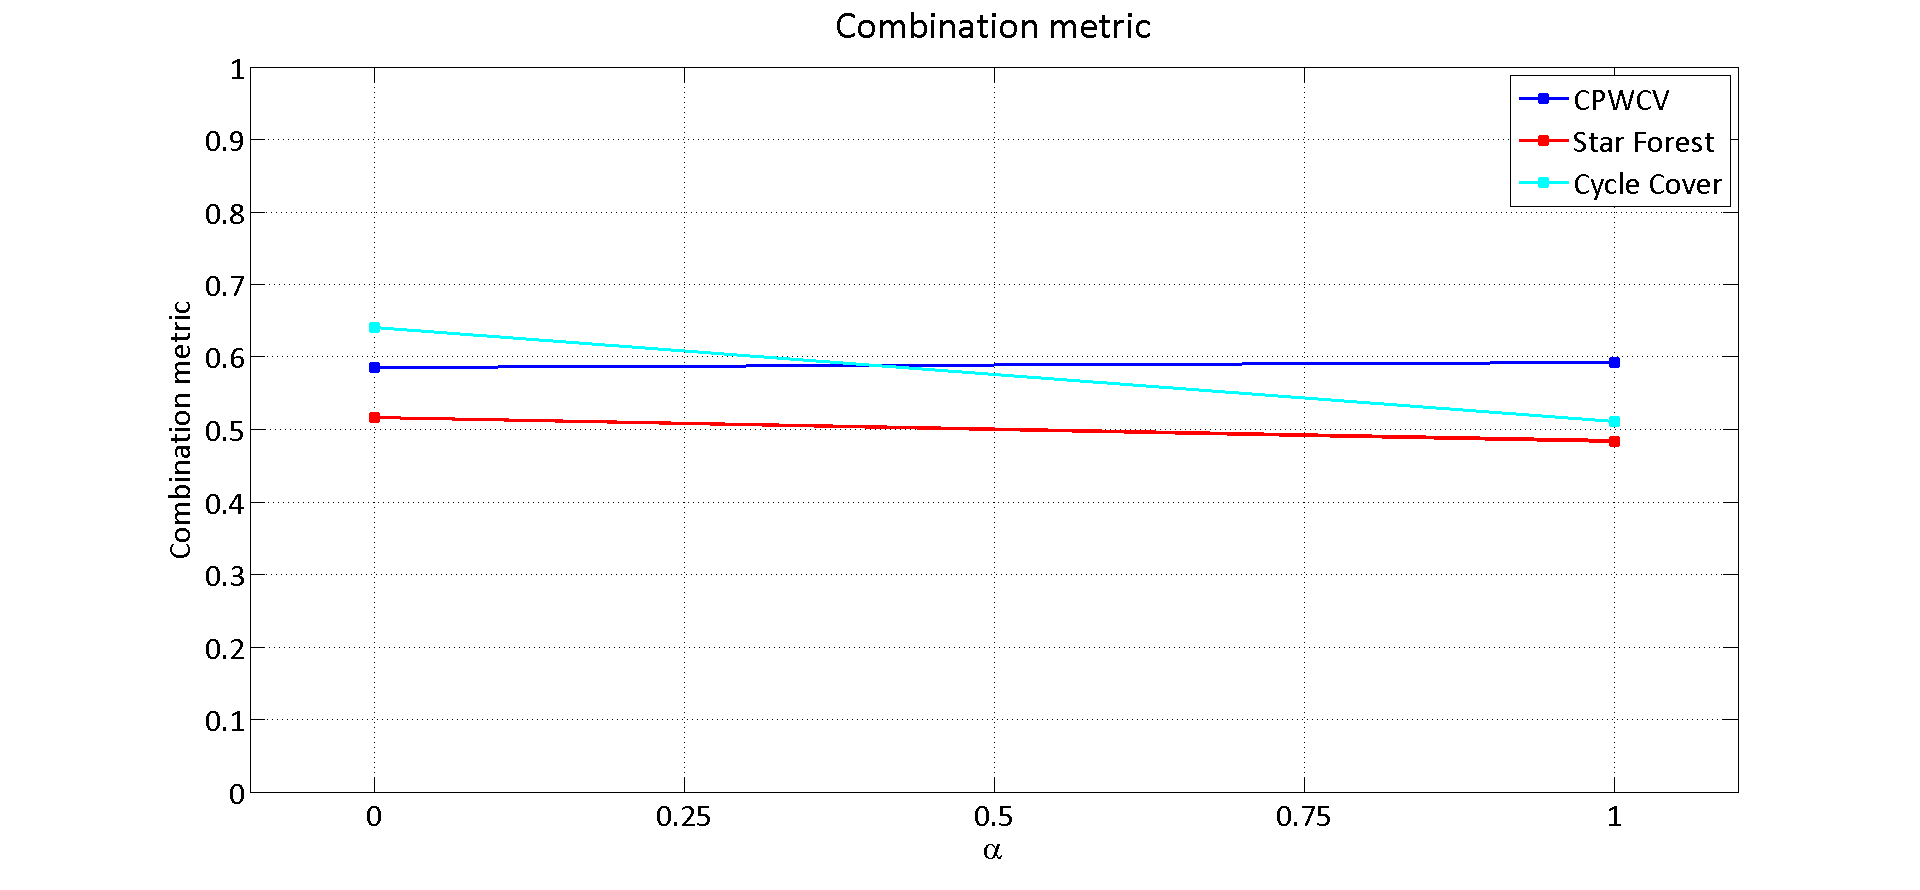
\includegraphics[scale=0.35]{img/impl_test/test_lexrank_jaccard/figures/combo_60.png}}
\caption{Combination metric: LexRank + Jaccard Similarity con 60 parole estratte.}
\label{combo_lexrank_jaccard_60}
\end{figure}
\begin{figure}
\centering
{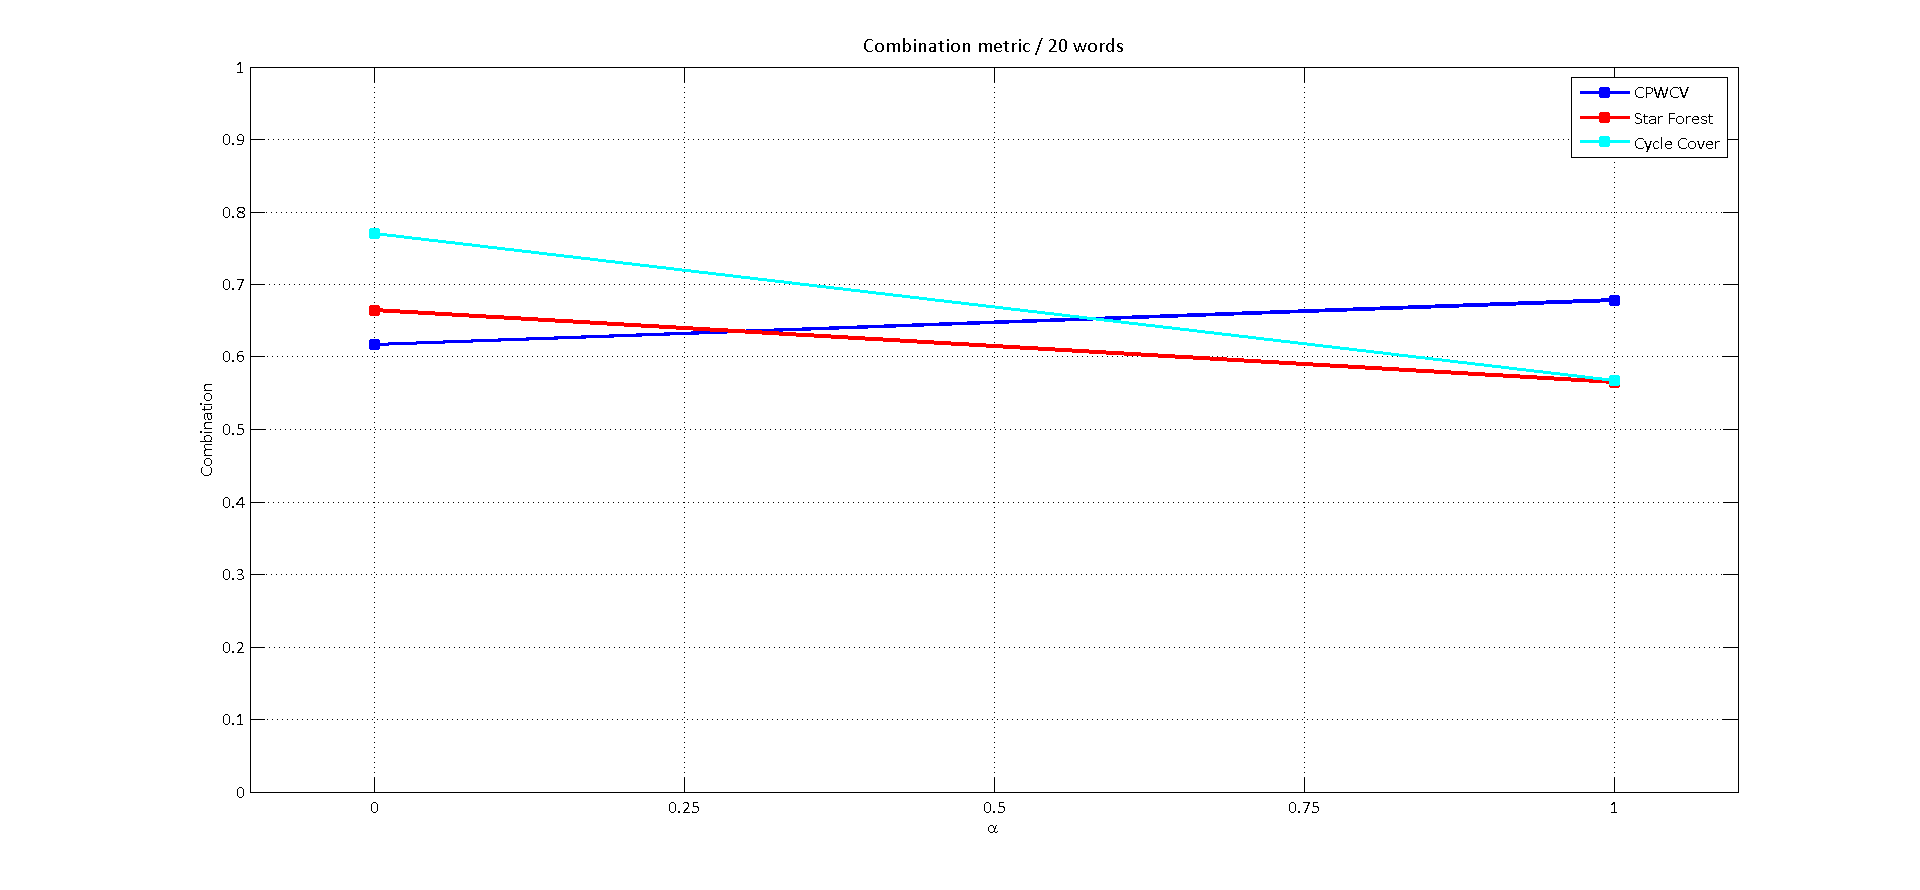
\includegraphics[scale=0.35]{img/impl_test/test_lexrank_cosine/figures/combo_20.png}}
\caption{Combination metric: LexRank + Cosine Similarity con 20 parole estratte.}
\label{combo_lexrank_cosine_20}
\end{figure}
\begin{figure}
\centering
{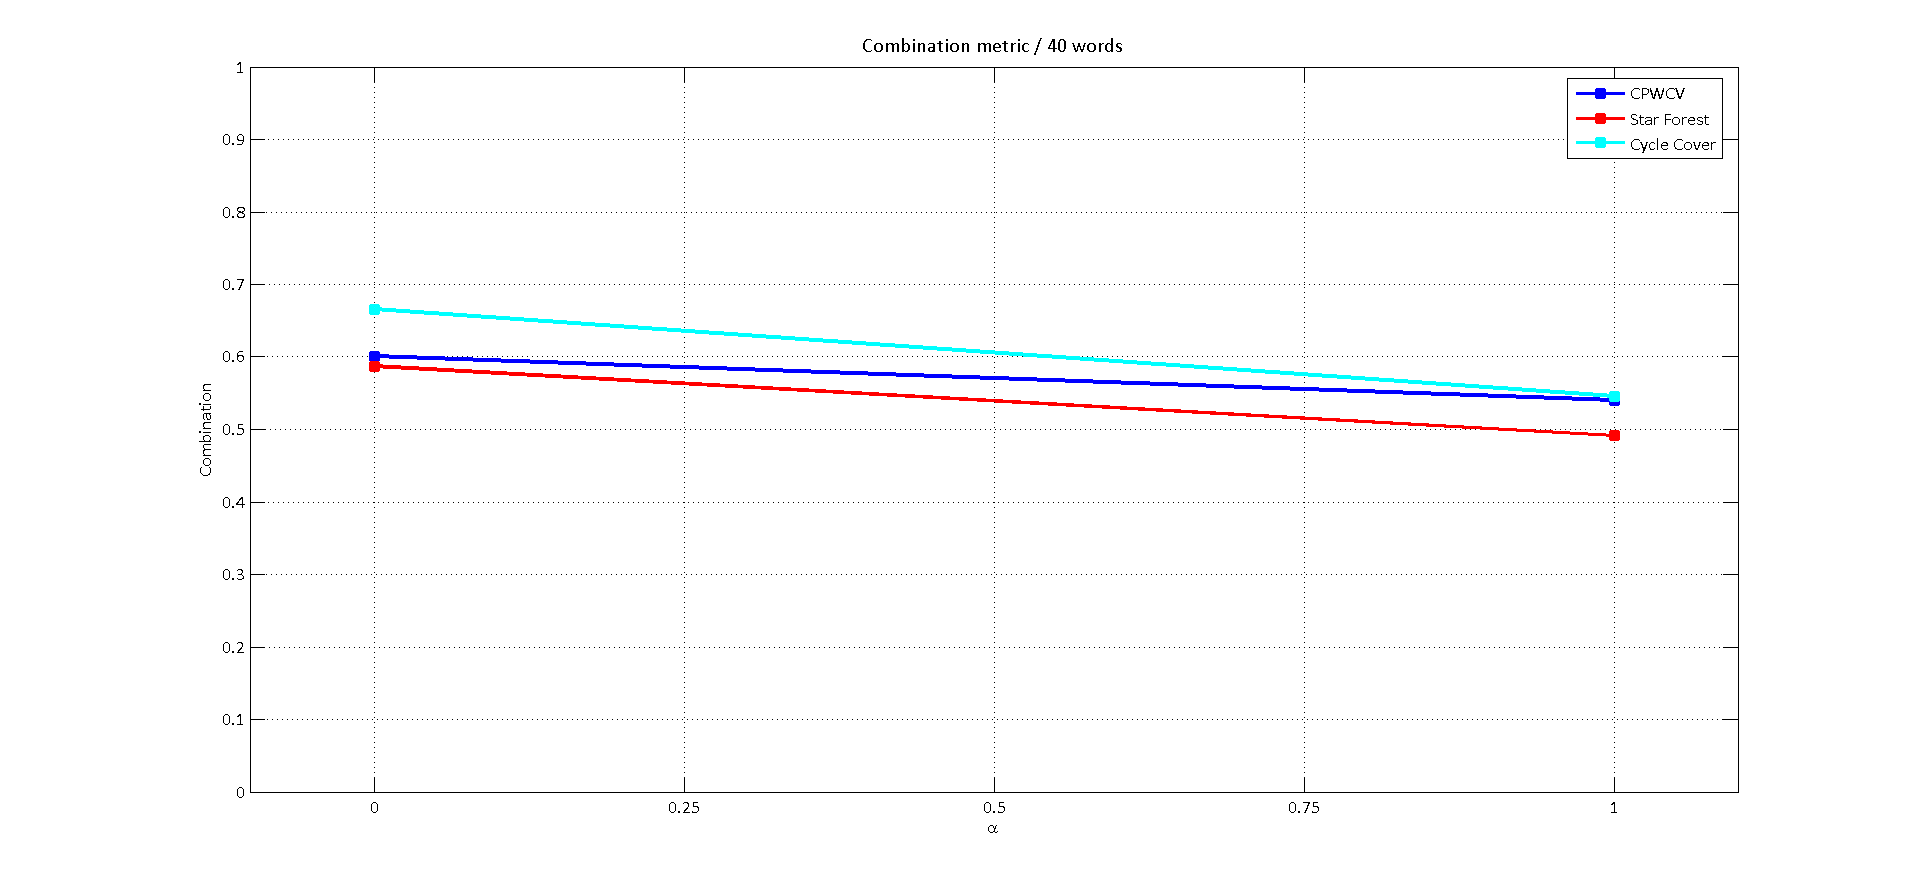
\includegraphics[scale=0.35]{img/impl_test/test_lexrank_cosine/figures/combo_40.png}}
\caption{Combination metric: LexRank + Cosine Similarity con 40 parole estratte.}
\label{combo_lexrank_cosine_40}
\end{figure}
\begin{figure}
\centering
{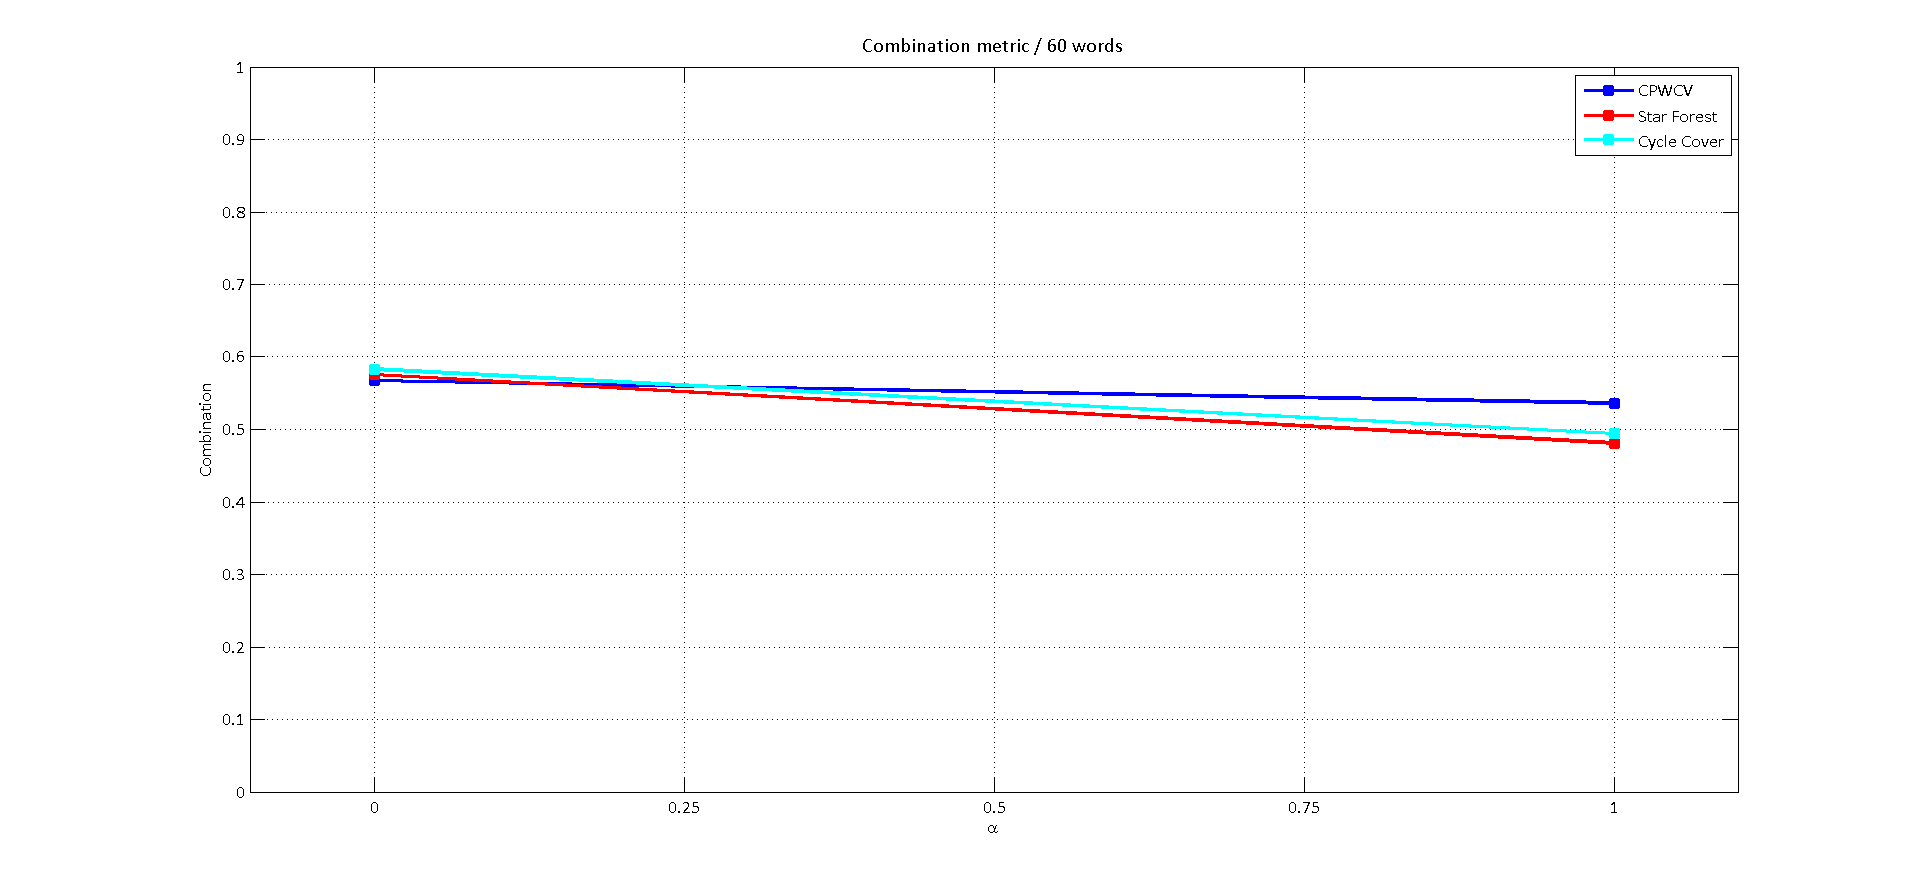
\includegraphics[scale=0.35]{img/impl_test/test_lexrank_cosine/figures/combo_60.png}}
\caption{Combination metric: LexRank + Cosine Similarity con 60 parole estratte.}
\label{combo_lexrank_cosine_60}
\end{figure}
\clearpage
\subsubsection{Space metric}
Nei risultati ottenuti, l'algoritmo CPWCV risulta essere l'algoritmo che produce disegni meno compatti, anche se la differenza con Star Forest e Cycle Cover non � eccessiva. Ovviamente, si ottengono valori diversi a seconda dell'utilizzo del bounding box o del convex hull. Quest'ultimo, infatti, ha un'area pi� piccola del bounding box, abbassando quindi il valore $1 - \dfrac{\mu}{\varphi}$. Ad ogni modo, comunque, si ottengono buoni risultati: i valori estremi (vicini a $0$ e $1$) possono infatti essere dannosi, poich� disegni troppo compatti comportano una difficolt� nella lettura di parole adiacenti, mentre disegni poco compatti possono risultare dispersivi.

\begin{figure}
\centering
{\includegraphics[scale=0.35]{img/impl_test/test_tf_jaccard/figures/spacemetric_20.png}}
\caption{Space metric: Term Frequency + Jaccard Similarity con 20 parole estratte.}
\label{sm_tf_jaccard_20}
\end{figure}
\begin{figure}
\centering
{\includegraphics[scale=0.35]{img/impl_test/test_tf_jaccard/figures/spacemetric_40.png}}
\caption{Space metric: Term Frequency + Jaccard Similarity con 40 parole estratte.}
\label{sm_tf_jaccard_40}
\end{figure}
\begin{figure}
\centering
{\includegraphics[scale=0.35]{img/impl_test/test_tf_jaccard/figures/spacemetric_60.png}}
\caption{Space metric: Term Frequency + Jaccard Similarity con 60 parole estratte.}
\label{sm_tf_jaccard_60}
\end{figure}
\begin{figure}
\centering
{\includegraphics[scale=0.35]{img/impl_test/test_tf_cosine/figures/spacemetric_20.png}}
\caption{Space metric: Term Frequency + Cosine Similarity con 20 parole estratte.}
\label{sm_tf_cosine_20}
\end{figure}
\begin{figure}
\centering
{\includegraphics[scale=0.35]{img/impl_test/test_tf_cosine/figures/spacemetric_40.png}}
\caption{Space metric: Term Frequency + Cosine Similarity con 40 parole estratte.}
\label{sm_tf_cosine_40}
\end{figure}
\begin{figure}
\centering
{\includegraphics[scale=0.35]{img/impl_test/test_tf_cosine/figures/spacemetric_60.png}}
\caption{Space metric: Term Frequency + Cosine Similarity con 60 parole estratte.}
\label{sm_tf_cosine_60}
\end{figure}
\begin{figure}
\centering
{\includegraphics[scale=0.35]{img/impl_test/test_tf_extended/figures/spacemetric_20.png}}
\caption{Space metric: Term Frequency + Extended Jaccard Similarity con 20 parole estratte.}
\label{sm_tf_extended_20}
\end{figure}
\begin{figure}
\centering
{\includegraphics[scale=0.35]{img/impl_test/test_tf_extended/figures/spacemetric_40.png}}
\caption{Space metric: Term Frequency + Extended Jaccard Similarity con 40 parole estratte.}
\label{sm_tf_extended_40}
\end{figure}
\begin{figure}
\clearpage
\centering
{\includegraphics[scale=0.35]{img/impl_test/test_tf_extended/figures/spacemetric_60.png}}
\caption{Space metric: Term Frequency + Extended Jaccard Similarity con 60 parole estratte.}
\label{sm_tf_extended_60}
\end{figure}
\begin{figure}
\centering
{\includegraphics[scale=0.35]{img/impl_test/test_tfidf_jaccard/figures/spacemetric_20.png}}
\caption{Space metric: TFIDF + Jaccard Similarity con 20 parole estratte.}
\label{sm_tfidf_jaccard_20}
\end{figure}
\begin{figure}
\centering
{\includegraphics[scale=0.35]{img/impl_test/test_tfidf_jaccard/figures/spacemetric_40.png}}
\caption{Space metric: TFIDF + Jaccard Similarity con 40 parole estratte.}
\label{sm_tfidf_jaccard_40}
\end{figure}
\begin{figure}
\centering
{\includegraphics[scale=0.35]{img/impl_test/test_tfidf_jaccard/figures/spacemetric_60.png}}
\caption{Space metric: TFIDF + Jaccard Similarity con 60 parole estratte.}
\label{sm_tfidf_jaccard_60}
\end{figure}
\begin{figure}
\centering
{\includegraphics[scale=0.35]{img/impl_test/test_tfidf_cosine/figures/spacemetric_20.png}}
\caption{Space metric: TFIDF + Cosine Similarity con 20 parole estratte.}
\label{sm_tfidf_cosine_20}
\end{figure}
\begin{figure}
\centering
{\includegraphics[scale=0.35]{img/impl_test/test_tfidf_cosine/figures/spacemetric_40.png}}
\caption{Space metric: TFIDF + Cosine Similarity con 40 parole estratte.}
\label{sm_tfidf_cosine_40}
\end{figure}
\begin{figure}
\centering
{\includegraphics[scale=0.35]{img/impl_test/test_tfidf_cosine/figures/spacemetric_60.png}}
\caption{Space metric: TFIDF + Cosine Similarity con 60 parole estratte.}
\label{sm_tfidf_cosine_60}
\end{figure}
\begin{figure}
\centering
{\includegraphics[scale=0.35]{img/impl_test/test_tfidf_extended/figures/spacemetric_20.png}}
\caption{Space metric: TFIDF + Extended Jaccard Similarity con 20 parole estratte.}
\label{sm_tfidf_extended_20}
\end{figure}
\begin{figure}
\centering
{\includegraphics[scale=0.35]{img/impl_test/test_tfidf_extended/figures/spacemetric_40.png}}
\caption{Space metric: TFIDF + Extended Jaccard Similarity con 40 parole estratte.}
\label{sm_tfidf_extended_40}
\end{figure}
\begin{figure}
\centering
{\includegraphics[scale=0.35]{img/impl_test/test_tfidf_extended/figures/spacemetric_60.png}}
\caption{Space metric: TFIDF + Extended Jaccard Similarity con 60 parole estratte.}
\label{sm_tfidf_extended_60}
\end{figure}
\clearpage
\begin{figure}[!htbp]
\centering
{\includegraphics[scale=0.35]{img/impl_test/test_lexrank_jaccard/figures/spacemetric_20.png}}
\caption{Space metric: LexRank + Jaccard Similarity con 20 parole estratte.}
\label{sm_lexrank_jaccard_20}
\end{figure}
\begin{figure}[!htbp]
\centering
{\includegraphics[scale=0.35]{img/impl_test/test_lexrank_jaccard/figures/spacemetric_40.png}}
\caption{Space metric: LexRank + Jaccard Similarity con 40 parole estratte.}
\label{sm_lexrank_jaccard_40}
\end{figure}
\begin{figure}[!htbp]
\centering
{\includegraphics[scale=0.35]{img/impl_test/test_lexrank_jaccard/figures/spacemetric_60.png}}
\caption{Space metric: LexRank + Jaccard Similarity con 60 parole estratte.}
\label{sm_lexrank_jaccard_60}
\end{figure}
\begin{figure}[!htbp]
\centering
{\includegraphics[scale=0.35]{img/impl_test/test_lexrank_cosine/figures/spacemetric_20.png}}
\caption{Space metric: LexRank + Cosine Similarity con 20 parole estratte.}
\label{sm_lexrank_cosine_20}
\end{figure}
\begin{figure}[!htbp]
\centering
{\includegraphics[scale=0.35]{img/impl_test/test_lexrank_cosine/figures/spacemetric_40.png}}
\caption{Space metric: LexRank + Cosine Similarity con 40 parole estratte.}
\label{sm_lexrank_cosine_40}
\end{figure}
\begin{figure}[!htbp]
\centering
{\includegraphics[scale=0.35]{img/impl_test/test_lexrank_cosine/figures/spacemetric_60.png}}
\caption{Space metric: LexRank + Cosine Similarity con 60 parole estratte.}
\label{sm_lexrank_cosine_60}
\end{figure}
\begin{figure}[!htbp]
\centering
{\includegraphics[scale=0.35]{img/impl_test/test_lexrank_extended/figures/spacemetric_20.png}}
\caption{Space metric: LexRank + Extended Jaccard Similarity con 20 parole estratte.}
\label{sm_lexrank_extended_20}
\end{figure}
\begin{figure}[!htbp]
\centering
{\includegraphics[scale=0.35]{img/impl_test/test_lexrank_extended/figures/spacemetric_40.png}}
\caption{Space metric: LexRank + Extended Jaccard Similarity con 40 parole estratte.}
\label{sm_lexrank_extended_40}
\end{figure}
\begin{figure}[!htbp]
\centering
{\includegraphics[scale=0.35]{img/impl_test/test_lexrank_extended/figures/spacemetric_60.png}}
\caption{Space metric: LexRank + Extended Jaccard Similarity con 60 parole estratte.}
\label{sm_lexrank_extended_60}
\end{figure}

\newpage 
\newpage
\newpage
\subsubsection{Running time}
Il tempo medio per l'elaborazione del testo e l'estrazione delle parole, calcolato per ogni algoritmo di ranking utilizzato, � espresso in tabella \ref{tab:ranking_time}. Si nota che l'algoritmo che impiega di pi� � TF-IDF, seguito da LexRank e Term Frequency, piuttosto veloce. TF-IDF risulta il meno veloce poich�, per ogni termine $t$, calcola il parametro $idf_{t}$, estratto dal corpus Brown. Tuttavia, rispetto a Term Frequency, tale algoritmo estrae parole pi� rilevanti.

Il tempo impiegato � il medesimo indipendentemente dal numero di parole estratte: le parole vengono comunque tutte classificate e inserite su una lista ordinata per punteggio. Poi vengono selezionate le prime $n$ parole, dove $n$ � il numero di parole scelto da visualizzare.
\begin{table}
\centering
\setlength{\tabcolsep}{12pt}
\begin{tabular}{cc}
\toprule
Algoritmo & Tempo [sec] \\
\midrule
Term Frequency 	&	$0.05$ \\						
\midrule
TF-IDF			& 	$0.43$ \\
\midrule
LexRank			&	$0.24$ \\
\bottomrule
\end{tabular}
\caption{Tempo d'esecuzione medio (espresso in secondi) di elaborazione del testo e classificazione delle parole.}
\label{tab:ranking_time}
\end{table}

Il tempo speso per il calcolo delle similarit� tra coppie di parole � indicato in tabella \ref{tab:simil_time}. Sono stati valutati i tempi di calcolo (espressi in $\mu s$) per 20,40 e 60 parole estratte. Gli algoritmi Cosine Similarity ed Extended Jaccard Similarity hanno quasi gli stessi tempi (in effetti i due algoritmi sono molto simili). La Jaccard Similarity impiega un p� di pi�.
\begin{table}
\centering
\begin{tabular}{cccc}
\toprule
\multirow{2}*{Parole estratte} & \multicolumn{3}{c}{Algoritmo} \\
\cmidrule(lr){2-4}
& Jaccard & Cosine & Extended Jaccard \\
\midrule
$20$ & $0.55$ & $0.34$& $0.36$\\
$40$ & $1.65$ & $0.98$ & $1.08$ \\
$60$ & $3$ & $1.88$ & $1.87$ \\
\bottomrule
\end{tabular}
\caption{Tempo d'esecuzione medio (espresso in $\mu s$) per il calcolo della similarit� per $20$,$40$ e $60$ parole estratte.}
\label{tab:simil_time}
\end{table}

In tabella \ref{tab:layout_time} sono riportati i tempi degli algoritmi di disegno. L'algoritmo pi� lento � Star Forest, mentre CPWCV e Cycle Cover sono paragonabili. In ogni caso, gli algoritmi di disegno sono piuttosto veloci e offrono buone prestazioni.
\begin{table}
\centering
\begin{tabular}{cccc}
\toprule
\multirow{2}*{Parole estratte} & \multicolumn{3}{c}{Algoritmo} \\
\cmidrule(lr){2-4}
& CPWCV & Star Forest & Cycle Cover \\
\midrule
$20$ & $3.93 \mu s$ & $0.095s$& $6.43 \mu s$\\
$40$ & $0.016 s$ & $0.18 s$ & $0.024s$ \\
$60$ & $0.048s$ & $0.274 s$ & $0.067 s$ \\
\bottomrule
\end{tabular}
\caption{Tempo d'esecuzione medio per la creazione della word cloud con $20$,$40$ e $60$ parole.}
\label{tab:layout_time}
\end{table}

La procedura di morphing � stata testata per un numero elevato di frame tra una word cloud ed un'altra, ovvero $150$. L'algoritmo risulta comunque piuttosto veloce (tabella \ref{tab:morphing_time}). I valori sono quasi uguali per 20 e 40 parole estratte, mentre il tempo aumenta per 60 parole estratte. 
\begin{table}
\centering
\setlength{\tabcolsep}{9pt}
\begin{tabular}{cc}
\toprule
Parole estratte & Tempo [$\mu s$] \\
\midrule
$20$ 	&	$0.53$ \\						
\midrule
$40$	& 	$0.6$\\
\midrule
$60$	&	$1.93$ \\
\bottomrule
\end{tabular}
\caption{Tempo d'esecuzione medio (espresso in $\mu s$) dell'algoritmo di morphing delle parole.}
\label{tab:morphing_time}
\end{table}

Nella tabella \ref{tab:clustering_time}, a pagina successiva, sono riportati i tempi d'esecuzione dell'algoritmo di clustering, che include anche la gestione delle variazioni tra cluster di layout successivi.
\begin{table}
\centering
\setlength{\tabcolsep}{9pt}
\begin{tabular}{cc}
\toprule
Parole estratte & Tempo [$\mu s$] \\
\midrule
$20$ 	&	$2.96$ \\						
\midrule
$40$	& 	$9.7$\\
\midrule
$60$	&	$19.27$ \\
\bottomrule
\end{tabular}
\caption{Tempo d'esecuzione medio (espresso in $\mu s$) dell'algoritmo di clustering per $20$,$40$ e $60$ parole estratte.}
\label{tab:clustering_time}
\end{table}

L'algoritmo di morphing che esegue l'aggiornamento dei colori frame per frame � leggermente pi� lento del morphing che aggiorna i bounding box delle parole. Questo perch� nell'implementazione vengono create ed accedute strutture dati pi� complesse (vedi tabella \ref{tab:colormorphing_time}).
\begin{table}
\centering
\setlength{\tabcolsep}{9pt}
\begin{tabular}{cc}
\toprule
Parole estratte & Tempo [$\mu s$] \\
\midrule
$20$ 	&	$3.52$ \\						
\midrule
$40$	& 	$7.58$\\
\midrule
$60$	&	$12.84$ \\
\bottomrule
\end{tabular}
\caption{Tempo d'esecuzione medio (espresso in $\mu s$) dell'algoritmo di morphing dei colori delle parole.}
\label{tab:colormorphing_time}
\end{table}

Per quanto riguarda la generazione dell'interfaccia grafica, questa fase, insieme all'elaborazione del testo e all'esecuzione dell'algoritmo di layout, � quella che incide maggiormente nel calcolo dei tempi. Ovviamente, al crescere del numero di parole, anche il tempo impiegato aumenta (vedi tabella \ref{tab:ui_time}).
\begin{table}
\centering
\setlength{\tabcolsep}{9pt}
\begin{tabular}{cc}
\toprule
Parole estratte & Tempo [$ s$] \\
\midrule
$20$ 	&	$0.4$ \\						
\midrule
$40$	& 	$0.48$\\
\midrule
$60$	&	$0.63$ \\
\bottomrule
\end{tabular}
\caption{Tempo medio (espresso in secondi) di creazione dell'interfaccia grafica per $20$,$40$ e $60$ parole.}
\label{tab:ui_time}
\end{table}

Infine, per valutare il tempo totale necessario a creare la word cloud dinamica, sono state considerate le configurazioni del sistema con gli algoritmi che, sulla base delle tabelle precedenti, hanno riportato le prestazioni peggiori e migliori in termini di consumo di tempo. Ci� vale ovviamente solo per gli algoritmi di estrazione delle parole, calcolo delle similarit� e disegno delle word cloud.

La configurazione peggiore � data dagli algoritmi TFIDF, Jaccard Similarity e Star Forest, mentre la configurazione migliore � data da Term Frequency, Cosine (o Extended Jaccard) Similarity e CPWCV (o Cycle Cover). Inoltre, come sopra, il numero di frame tra una word cloud e la successiva � pari a $150$.

I risultati ottenuti sono del tutto ragionevoli e sono riportati in tabella \ref{tab:total_time}.

\begin{table}
\centering
\setlength{\tabcolsep}{9pt}
\begin{tabular}{ccc}
\toprule
Parole estratte & Caso peggiore & Caso migliore  \\
\midrule
$20$ & $2.65$ & $0.77$\\
$40$ & $3.01$ & $0.94$\\
$60$ & $3.66$ & $1.25$\\
\bottomrule
\end{tabular}
\caption[Tempo d'esecuzione medio (espresso in secondi) per la creazione della word cloud con $20$,$40$ e $60$ parole.]{Tempo d'esecuzione medio (espresso in secondi) per la creazione della word cloud con $20$,$40$ e $60$ parole. Configurazione caso peggiore: TFIDF, Jaccard Similarity e Star Forest. Configurazione caso migliore: Term Frequency, Cosine Similarity e CPWCV.}
\label{tab:total_time}
\end{table}
%...

%%APPENDICI==============================================
% \appendix
% \input{appendiceA}
%...

%%BIBLIOGRAFIA============================================
\normalsize
\newpage
\bibliographystyle{unsrt}
\bibliography{bibliografia}

\end{document}
